%======================================================================
\chapter{Introduction}
%======================================================================

\code{radiosynth} computes \emph{synthetic radio images} of the solar corona from the
output of a magnetohydrodynamic (MHD) model. For every pixel of the image it
traces the radio ray backwards from the observer through the model plasma.
The ray bends because the refractive index of a plasma depends on the electron
density. The code adds up the thermal free--free (bremsstrahlung) emission along
the curved path. It also computes \textbf{thermal gyroresonance}
emission from the magnetic field of the model, together with magnetised free--free
emission, in total intensity and circular polarisation (Stokes $V$;
Chapter~\ref{chap:gr}), and the \textbf{gyrosynchrotron} emission of
prescribed fast electrons, computed with the public fast gyrosynchrotron codes
(Chapter~\ref{chap:gs}); the three can be combined in one radiative
transfer (Chapter~\ref{chap:combined}).

This manual describes the second version of \code{radiosynth} (package version 2.2.0).
\code{radiosynth} is written by Soumitra Hazra and is free software, distributed under
the GNU General Public License, version 3 or (at your option) any later version. It
follows previously existing codes and published algorithms --- the radio-wave imaging
module of BATS-R-US (Benkevitch et al.\ 2010; Moschou et al.\ 2018), the pyPLUTO reader
of the PLUTO code and the fast gyrosynchrotron codes of Fleishman \& Kuznetsov, which it
calls as a library --- and it was developed with the help of large language models. Its
results are checked against analytic solutions and independent calculations by the
test suite (Chapter~\ref{chap:validation}). If you use it in a publication, please cite the
software and the papers on which its algorithms are based (Benkevitch et al.\ 2010;
Moschou et al.\ 2018; and, for gyrosynchrotron emission, Kuznetsov \& Fleishman 2021).

The algorithm is the one built into the BATS-R-US code of the Space Weather Modeling
Framework, written by L.~Benkevitch (Benkevitch et al.\ 2010) and extended to
bremsstrahlung emission by Moschou et al.\ (2018). In BATS-R-US it runs \emph{inside} the
simulation (\code{ModWritePlotRadioWave.f90}, \code{ModRadioWaveImage.f90} and
\code{ModUserAwsom.f90}). \code{radiosynth} is an independent re-implementation in Python
that works on \emph{saved} model output. You can therefore use it

\begin{itemize}[itemsep=1pt]
  \item on any BATS-R-US snapshot (Tecplot or IDL format) after the run has finished;
  \item on output of \textbf{PLUTO}, Cartesian or spherical, 3D or 2.5D axisymmetric;
  \item on any other model whose electron density and temperature you can load
        into NumPy arrays (MAS, Athena++, FLASH, analytic models, \ldots);
  \item on models of \textbf{other stars}: coordinates in stellar radii, an observer at a
        distance in parsec, spectra, spectral indices, rotational modulation and VLBI-scale
        images (Chapter~\ref{chap:stellar});
  \item on \textbf{1D} (spherically symmetric) models: radial brightness profiles, spectra
        and images from a single row of rays (Chapter~\ref{chap:sym}).
\end{itemize}

Each emission mechanism has its own folder; everything they share (readers, grids,
geometry, ray tracing, figures, comparison with observations) is in one common folder
(Section~\ref{sec:layout}). It also provides tools for comparing the results with observations: solar coordinates,
overlays and statistics (Chapters~\ref{chap:figs} and~\ref{chap:plutoobs}).

\section{What the code does}

\begin{enumerate}[itemsep=2pt]
  \item \textbf{Reads} the MHD output and converts it to electron density
        $n_e$ [m$^{-3}$] and electron temperature $T_e$ [K] on a grid. The grid is
        either Cartesian (\code{MHDGrid}) or spherical (\code{SphericalGrid}).
  \item \textbf{Sets up an image plane} through the Sun's centre, perpendicular to the
        observer's line of sight. It has $n_x\times n_y$ pixels covering
        $X_\text{size}\times Y_\text{size}$ solar radii. One ray is sent from the
        observer through the centre of each pixel.
  \item \textbf{Traces each ray} through the plasma with the Boris-type integrator
        of Benkevitch et al.\ (2010). The step size is adapted to the curvature of
        the ray. Near the critical surface, where the plasma frequency equals the
        observing frequency, the ray is reflected along a parabola.
  \item \textbf{Integrates the emission} along each ray:
        $I_\nu=\int\kappa_\nu B_\nu\,ds$ in the BATS-R-US (optically thin) mode, or
        the full radiative-transfer solution $I_\nu=\int B_\nu e^{-\tau}\,d\tau$.
  \item \textbf{Returns} images of intensity, brightness temperature and optical depth,
        the total flux density, and how each ray ended. These can be saved as
        NPZ, Tecplot ASCII (same layout as BATS-R-US) or FITS, and plotted.
\end{enumerate}

\section{Package layout}\label{sec:layout}

The package is organised in six folders: one common folder used by every mechanism,
one folder per emission mechanism, and one folder that combines them (Figure~\ref{fig:layout}). A mechanism folder
only contains its own physics and calls the common machinery as subroutines; the
common folder knows the mechanisms only through a registry
(\code{common/mechanism.py}), so a new mechanism is added by creating a new folder.

\begin{figure}[h]\centering
\begin{tikzpicture}[font=\small, box/.style={draw=accent, rounded corners=2pt, fill=notebg,
  align=left, inner sep=5pt, text width=#1}, box/.default=3.6cm, >=Stealth]
\node[box=15.2cm] (common) at (0,0) {\textbf{common/}\quad constants, magnetoionic, grid (+$\vect B$, scalars), fields ($|\vect J|$), readers, pluto, contrib/pyPLUTO,
 mechanism (registry), emission (interface), raytrace (refractive), straight (straight rays), image,
 figures (orientation, comparison with observations), stellar, fitsio, cli};
\node[box=3.0cm] (simp) at (-6.0,2.4) {\textbf{simplistic/}\\ emission};
\node[box=3.0cm] (ff) at (-2.1,2.4) {\textbf{bremsstrahlung/}\\ emission\\ magnetized (o/x)\\ wind};
\node[box=3.0cm] (gr) at (1.8,2.4) {\textbf{gyroresonance/}\\ opacity\\ transfer\\ image};
\node[box=3.0cm] (gs) at (5.7,2.4) {\textbf{gyrosynchrotron/}\\ library\\ electrons\\ image};
\node[box=4.6cm] (cb) at (0.4,4.6) {\textbf{combined/}\\ coefficients (GS per voxel)\\ image (CombinedImage)};
\draw[->,thick,accent] (cb.south) -- (gr.north);
\draw[->,thick,accent] (cb.south) -- (gs.north);
\draw[->,thick,accent] (cb.south) -- (ff.north);
\node[draw=gray, dashed, rounded corners=2pt, align=center, font=\scriptsize, inner sep=4pt] (lib) at (6.2,4.6)
  {fast GS codes (Kuznetsov \& Fleishman 2021)\\ compiled library, GPL-3, not bundled};
\draw[->,thick,accent] (simp.south) -- (simp.south |- common.north);
\draw[->,thick,accent] (ff.south) -- (ff.south |- common.north);
\draw[->,thick,accent] (gr.south) -- (gr.south |- common.north);
\draw[->,thick,accent] (gs.south) -- (gs.south |- common.north);
\draw[->,thick,gray,dashed] (gs.north) -- node[left,font=\scriptsize]{ctypes} (lib.south);
\draw[->,thick,accent,dashed] (gr.west) -- node[below,font=\scriptsize]{uses} (ff.east);
\node[font=\scriptsize,gray] at (0,-1.05) {refractive ray tracer: simplistic, bremsstrahlung \quad$\cdot$\quad straight rays + polarisation: gyroresonance, gyrosynchrotron};
\end{tikzpicture}
\caption{Package layout. Arrows: ``calls''. The gyroresonance folder also uses the
magnetised free--free coefficients of the bremsstrahlung folder, because both
contributions are computed together. The gyrosynchrotron folder hands the lines of sight
to the public fast gyrosynchrotron codes, which are compiled once on the user's
machine. The combined folder uses the other three to put free--free, gyroresonance and
gyrosynchrotron emission into one radiative transfer.}\label{fig:layout}
\end{figure}

\begin{center}\small
\begin{tabularx}{\textwidth}{@{}l X@{}}
\toprule
File & Content \\
\midrule
\multicolumn{2}{@{}l}{\emph{radiosynth/common/ --- shared by all mechanisms}}\\
\code{constants.py} & Physical constants; critical density and plasma frequency. \\
\code{magnetoionic.py} & Cold-plasma magneto-ionic theory: $X$, $Y$, mode polarisation, Appleton--Hartree index, cutoffs. \\
\code{grid.py} & \code{MHDGrid} (Cartesian) and \code{SphericalGrid}: $n_e$, $T_e$, gradients and (optionally) $\vect B$ and named scalar fields; fast trilinear sampling. \\
\code{fields.py} & Derived fields: $\nabla\times\vect B$ and the current density $|\vect J|$. \\
\code{symmetric.py} & 1D (spherically symmetric) models: grid from a profile or a text table, fast symmetric images, radial profiles. \\
\code{readers.py} & BATS-R-US Tecplot/IDL readers, unit handling, resampling, \code{load\_mhd} (\code{with\_b=True} reads $\vect B$). \\
\code{pluto.py} & PLUTO \code{.dbl}/\code{.flt}/\code{.vtk} readers, units, \code{bx1..bx3}, \code{load\_pluto}. \\
\code{contrib/pyPLUTO.py} & The classic pyPLUTO reader shipped with PLUTO (bundled, with a one-line fix). \\
\code{mechanism.py} & Registry of emission mechanisms. \\
\code{emission.py} & \code{EmissionModel}: the interface used by the refractive tracer. \\
\code{raytrace.py} & \code{trace\_rays}: refractive ray tracer and intensity integrator (port of \code{ray\_path}). \\
\code{straight.py} & Straight-ray sampler for polarised transfer. \\
\code{image.py} & Image geometry, \code{make\_radio\_image}, \code{RadioImage}, \code{trace\_paths}. \\
\code{figures.py} & Figures (Moschou et al.\ 2018 style), solar ephemeris and orientation, comparison with observations. \\
\code{stellar.py} & Stars: viewing geometry, images at a distance, spectra, spectral index, rotational modulation. \\
\code{fitsio.py} & FITS reading/writing (astropy if installed, otherwise built in). \\
\code{cli.py} & Command line (\code{python -m radiosynth}). \\
\multicolumn{2}{@{}l}{\emph{radiosynth/simplistic/}}\\
\code{emission.py} & Benkevitch et al.\ (2010) emissivity. \\
\multicolumn{2}{@{}l}{\emph{radiosynth/bremsstrahlung/}}\\
\code{emission.py} & Thermal free--free coefficients (Gaunt factor 10 or Dulk 1985). \\
\code{magnetized.py} & Free--free absorption of the o- and x-modes. \\
\code{wind.py} & Analytic isothermal-wind solution (validation, stars). \\
\multicolumn{2}{@{}l}{\emph{radiosynth/gyroresonance/}}\\
\code{opacity.py} & Optical depth of the harmonic layers $\nu=s\nu_B$ for both modes. \\
\code{transfer.py} & Polarised transfer along straight rays: layers + free--free, Stokes $I$ and $V$. \\
\code{image.py} & \code{make\_gr\_image}, \code{GRImage}. \\
\multicolumn{2}{@{}l}{\emph{radiosynth/gyrosynchrotron/}}\\
\code{library.py} & Finds, builds and loads the public fast gyrosynchrotron codes (ctypes). \\
\code{electrons.py} & \code{FastElectrons}: the prescription of the fast electrons; rules for $n_b$. \\
\code{image.py} & \code{make\_gs\_image}, \code{GSImage}. \\
\multicolumn{2}{@{}l}{\emph{radiosynth/combined/}}\\
\code{coefficients.py} & Per-voxel gyrosynchrotron optical depth and emission from the fast GS codes. \\
\code{image.py} & \code{make\_combined\_image}, \code{CombinedImage}: free--free + gyroresonance + gyrosynchrotron in one transfer. \\
\midrule
\code{radiosynth/\_\_init\_\_.py} & Public interface; the short module paths (\code{radiosynth.grid}, \ldots) also work. \\
\code{examples/} & \code{synthetic\_corona.py}, \code{demo.py}, \code{moschou\_figures.py}, \code{stellar\_example.py}, \code{active\_region.py}, \code{gyroresonance\_example.py}, \code{gyrosynchrotron\_example.py}, \code{combined\_example.py}, \code{symmetric\_example.py}. \\
\code{tests/} & \code{validate.py}, \code{test\_readers.py}, \code{test\_pluto.py}, \code{test\_orientation.py}, \code{test\_stellar.py}, \code{test\_gyroresonance.py}, \code{test\_gyrosynchrotron.py}, \code{test\_refraction\_compare.py}, \code{test\_combined.py}, \code{test\_symmetric.py}. \\
\bottomrule
\end{tabularx}
\end{center}

\begin{note}[Short module paths]
The modules in \code{common/} can also be imported by their short paths, e.g.\
\code{from radiosynth.constants import R\_SUN} or \code{rs.figures}. The analytic wind
functions live in \code{bremsstrahlung/wind.py} and are also available as
\code{rs.stellar.wind\_flux\_density}.
\end{note}

%======================================================================
\chapter{Emission mechanisms}\label{chap:mech}
%======================================================================

\begin{center}\small
\begin{tabularx}{\textwidth}{@{}l l l X@{}}
\toprule
Mechanism (folder) & Needs & Rays & Use it for \\
\midrule
\code{simplistic} & $n_e$ & refracted & visualising refraction and the critical layer (dimensionless) \\
\code{bremsstrahlung} & $n_e$, $T_e$ & refracted & metre to centimetre waves from the quiet corona, CMEs, stellar winds \\
\code{gyroresonance} & $n_e$, $T_e$, $\vect B$ & straight & active regions at 1--20\,GHz, magnetic-field diagnostics, circular polarisation \\
\code{gyrosynchrotron} & $n_e$, $T_e$, $\vect B$ + fast electrons & straight & flares, CME cores, active stars: emission of mildly relativistic electrons (needs the public fast GS codes) \\
\code{combined} & all of the above & straight (+ optional free--free refraction) & the three processes together, absorbing each other (Chapter~\ref{chap:combined}) \\
\bottomrule
\end{tabularx}
\end{center}

Each folder has the same entry point, \code{make\_image(grid, frequencies, ...)}:
\begin{lstlisting}[style=pyex]
import radiosynth as rs
g  = rs.load_mhd("3d__mhd_ar.dat", with_b=True)     # B needed only for gyroresonance

a = rs.simplistic.make_image(g, "80MHz", observer=(-215, 0, 0))
b = rs.bremsstrahlung.make_image(g, "80MHz, 17GHz", transfer="full")   # = rs.make_radio_image
c = rs.gyroresonance.make_image(g, "5GHz, 17GHz", x_size=0.5, y_size=0.5)  # = rs.make_gr_image
e = rs.FastElectrons(nb=rs.gyrosynchrotron.in_sphere((-1.04, 0, 0), 0.02, 1e7), delta=3.5)
d = rs.gyrosynchrotron.make_image(g, "5GHz, 17GHz", e, x_size=0.5, y_size=0.5)  # = rs.make_gs_image

rs.available_mechanisms()  # ['bremsstrahlung', 'gyroresonance', 'gyrosynchrotron', 'simplistic']
\end{lstlisting}
and on the command line \code{--mechanism simplistic|bremsstrahlung|gyroresonance|gyrosynchrotron}
(\code{--list-mechanisms} prints them). All return a \code{RadioImage} (the
gyroresonance and gyrosynchrotron ones a \code{GRImage}/\code{GSImage}, which add Stokes $V$), so the plotting, FITS output,
orientation and comparison tools of Chapters~\ref{chap:figs}--\ref{chap:stellar} work
for all of them.

\paragraph{Free--free \emph{and} gyroresonance in one image.} Both are thermal processes
of the same electrons, so in a real active region they absorb each other's radiation:
an optically thick gyroresonance layer hides the free--free emission behind it, and dense
free--free plasma in front of a layer attenuates it. The gyroresonance image therefore
includes free--free emission and absorption by default (\code{mechanisms="gr+ff"}); the
separate contributions are available for diagnosis (\code{"gr"}, \code{"ff"}), see
Section~\ref{sec:grmech}. Note that the combined image is \emph{not} the sum of the two
separate ones.

\paragraph{Refracted or straight rays?} Below about 1\,GHz the rays bend appreciably in
the corona, and the free--free image needs the refractive tracer
(\code{bremsstrahlung}). Gyroresonance layers form where $\nu=s\nu_B$ with $s=2$--4, at
field strengths of hundreds of gauss, where $\nu\gg\nu_p$: refraction is negligible
there, and all gyroresonance codes use straight rays. The \code{gyroresonance} folder
flags pixels where this assumption becomes questionable (\code{x\_flag},
Section~\ref{sec:grout}). For the mechanisms with refractive ray tracing the effect of
refraction can be measured directly: \code{no\_refraction=True} gives straight lines of
sight, and \code{compare\_refraction} computes and plots both
(Section~\ref{sec:refcmp}).

\paragraph{Adding a mechanism.} Create a folder \code{radiosynth/mymech/} with an
\code{\_\_init\_\_.py} that calls
\begin{lstlisting}[style=pyex]
from ..common.mechanism import Mechanism, register
MECHANISM = register(Mechanism("mymech", coefficients=my_coefficients,
                               make_image=my_make_image, description="..."))
\end{lstlisting}
\code{my\_coefficients(ne, te, freq, length\_unit)} returns $(\kappa, S)$ if the
mechanism can be used with the refractive tracer (then \code{emission="mymech"} works
everywhere); otherwise set it to \code{None} and provide your own driver, as the
gyroresonance folder does with the straight-ray sampler.

%======================================================================
\chapter{Installation}
%======================================================================

\code{radiosynth} is pure Python. It needs

\begin{itemize}[itemsep=1pt]
  \item Python $\ge$ 3.8, \code{numpy}, \code{scipy}, \code{matplotlib};
  \item optional: \code{astropy} (used for FITS files if installed; a built-in reader and
        writer is used otherwise), \code{pytecplot} (only for binary Tecplot
        \code{.plt}/\code{.szplt} files; needs a Tecplot 360 licence), \code{sunpy}
        (optional: the ephemeris is built in; sunpy is used if present, and for rotating observed maps), and
        \code{ffmpeg} (only for MP4 animations; GIF needs nothing extra).
\end{itemize}

Unzip the package and either work in its top directory or add it to your path:

\begin{lstlisting}
unzip radiosynth.zip -d ~/codes/radiosynth
cd ~/codes/radiosynth
pip install numpy scipy matplotlib astropy      # if not already installed
python tests/validate.py                         # optional self-test (about 10 s)
\end{lstlisting}

To import it from anywhere, either set \code{export PYTHONPATH=\$HOME/codes/radiosynth:\$PYTHONPATH}
or, in a script, \code{sys.path.insert(0, "/home/you/codes/radiosynth")}.

%======================================================================
\chapter{Quick start}
%======================================================================

\section{From Python}

\begin{lstlisting}[style=pyex]
import radiosynth as rs

# 1. read the model (format detected from the file name / directory)
grid = rs.load_mhd("box_mhd_4_n00155869.dat")    # BATS-R-US Tecplot ASCII
# grid = rs.load_mhd("pluto_run/out")             # PLUTO output directory

# 2. make the image
img = rs.make_radio_image(grid, "42.3MHz, 80MHz, 150MHz, 1GHz",
                          observer=(-215, 0, 0),     # Earth-like, R_sun
                          x_size=6, y_size=6,        # field of view, R_sun
                          nx=256, ny=256,            # pixels
                          transfer="full",           # or "thin" (BATS-R-US)
                          n_workers=8)               # CPU cores

# 3. use / save the result
img.plot("tb", path="radio_Tb.png")                  # brightness temperature
img.save_npz("radio.npz")
print(img.flux_density_sfu)                          # total flux, sfu
\end{lstlisting}

\section{From the command line}

\begin{lstlisting}
python -m radiosynth box_mhd_4_n00155869.dat --freq "80MHz, 150MHz, 17GHz" \
       --observer -215 0 0 --size 6 6 --npix 256 256 --workers 8 --plot

python -m radiosynth pluto_run/out --freq "80MHz, 150MHz" \
       --definitions pluto_run/definitions.h --transfer full --plot --out run1
\end{lstlisting}

As it runs, the program prints:

\begin{itemize}[itemsep=1pt]
  \item how it interpreted the input (variables used, units, typical values at
        $r\approx1.1\,\rsun$);
  \item one line per frequency, with the run time and the mean number of steps per ray;
  \item a summary of the maximum intensity, the maximum $T_b$ and the flux, with
        counts of how the rays ended.
\end{itemize}

\textbf{Always check the printed $n_e$ and $T_e$ values}. Typical low-corona values are
$n_e\sim10^{14}$--$10^{15}$\,m$^{-3}$ and $T_e\sim1$--$2$\,MK. Values far from this
almost always mean wrong units.

%======================================================================
\chapter{Preparing the input}
%======================================================================

The ray tracer needs only two fields: the \textbf{electron density} $n_e$ and the
\textbf{electron temperature} $T_e$, with coordinates in solar radii. The readers below
produce them from the usual MHD variables. Table~\ref{tab:inputs} summarises the
supported inputs.

\begin{table}[h]
\centering\small
\begin{tabularx}{\textwidth}{@{}l l X@{}}
\toprule
Model & Format & How to load \\
\midrule
BATS-R-US & Tecplot ASCII \code{.dat}/\code{.tec} (box, 3d, cut) & \code{rs.load\_mhd("file.dat")} \\
BATS-R-US & Tecplot binary \code{.plt} & \code{rs.load\_mhd("file.plt")} (needs \code{pytecplot}) \\
BATS-R-US & IDL \code{.out} (ascii, real4, real8) & \code{rs.load\_mhd("file.out")} \\
PLUTO & \code{.dbl}/\code{.flt} + \code{grid.out} + \code{dbl.out}/\code{flt.out} & \code{rs.load\_mhd("outdir")} or \code{rs.load\_pluto("outdir", nout=...)} \\
PLUTO & legacy VTK \code{.vtk} & \code{rs.load\_mhd("data.0010.vtk")} \\
any & NumPy arrays, Cartesian & \code{rs.MHDGrid(x, y, z, ne, te)} \\
any & NumPy arrays, spherical & \code{rs.SphericalGrid(r, theta, phi, ne, te)} \\
any & saved grid \code{.npz} & \code{rs.load\_mhd("grid.npz")} \\
\bottomrule
\end{tabularx}
\caption{Supported inputs.}\label{tab:inputs}
\end{table}

%----------------------------------------------------------------------
\section{BATS-R-US output}
%----------------------------------------------------------------------

\subsection*{Recommended: a uniform box plot}
BATS-R-US \code{3d} plots are written on the AMR grid, so the points are not on a tensor
grid. The best input is a \emph{box} plot with a fixed resolution. Put this in
\code{PARAM.in} (SC component):

\begin{lstlisting}
#SAVEPLOT
1                       nPlotFile
box mhd tec             StringPlot   (or: box mhd idl)
-1                      DnSavePlot
3600.0                  DtSavePlot
0.0  0.0  0.0           Coord1, Coord2, Coord3 of the box centre
8.0  8.0  8.0           Size of the box (R_sun)
0.0  0.0  0.0           Rotation angles
0.02                    dx (R_sun)  -> uniform 400^3 grid
\end{lstlisting}

The \code{mhd} variable set contains \code{Rho}, \code{U}, \code{B}, \code{P} and, in
AWSoM runs with electron pressure, \code{Pe}. That is all the code needs. A resolution
of 0.02--0.03\,\rsun{} is adequate. Use a finer box if you want sharp images at the
higher frequencies.

\subsection*{How the variables are interpreted}

\begin{itemize}[itemsep=2pt]
\item \textbf{Coordinates}: variables named \code{X}, \code{Y}, \code{Z} (case and units
      in brackets ignored), assumed in \rsun.
\item \textbf{Density}: the first of \code{ne}, \code{n\_e}, \code{rho}, \code{n},
      \code{dens}, \ldots{} (or \code{--density-var}). The unit is taken from the name
      (\code{"Rho [g/cm\^{}3]"}), from the IDL header, or from \code{--density-unit}.
      If none of these is available, the unit is guessed from the magnitude of the
      values near $r=1.1\,\rsun$. A mass density is converted with
      $n_e=\rho/(\mu\, m_p)$; $\mu=1$ by default, as in BATS-R-US.
\item \textbf{Temperature}, in this order of priority:
  \begin{enumerate}[itemsep=0pt]
    \item a \code{Te} variable (K);
    \item $T_e=P_e/(n_e k_B)$ from \code{Pe};
    \item $T_e=P/(2n_e k_B)$ from the total pressure \code{P}, i.e.\ assuming $T_e=T_i$;
    \item a \code{T}/\code{temp} variable;
    \item the constant \code{te\_const}.
  \end{enumerate}
  Pressures are in dyn\,cm$^{-2}$ unless the name says otherwise.
\end{itemize}

\subsection*{Example: your Tecplot file}
The original script \code{Radio\_Emsssion\_Calculation\_batsrus.py} loaded
\code{3d\_\_mhd\_2\_t00120000\_n00155869.plt} with \code{pytecplot}. The same file can be
used directly:

\begin{lstlisting}[style=pyex]
import radiosynth as rs
grid = rs.load_mhd("3d__mhd_2_t00120000_n00155869.plt")       # via pytecplot
# if the file has no pressure, give a temperature:
grid = rs.load_mhd("3d__mhd_2_t00120000_n00155869.plt", te_const=1.5e6)
\end{lstlisting}

If you have no Tecplot licence, convert the file to ASCII with \code{preplot}/Tecplot or
write \code{tec} ASCII plots from BATS-R-US. ASCII files are read without \code{pytecplot}.

\subsection*{AMR / scattered points}
If the points do not form a tensor grid, \code{load\_mhd} resamples them to a uniform box
of \code{resample\_shape} (default $160^3$). The default \code{"linear"} method
interpolates $\log n_e$ on a Delaunay triangulation. It is accurate but slow for many
millions of points. \code{"nearest"} is fast. Limit the box with \code{resample\_box}:

\begin{lstlisting}[style=pyex]
grid = rs.load_mhd("3d__mhd_1_n00010000.out", resample_shape=(300, 300, 300),
                   resample_box=((-4, 4), (-4, 4), (-4, 4)), resample_method="linear")
grid.to_npz("grid_n10000.npz")       # save once, reuse fast: rs.load_mhd("grid_n10000.npz")
\end{lstlisting}

%----------------------------------------------------------------------
\section{PLUTO output}
%----------------------------------------------------------------------

\subsection*{Files read}
PLUTO writes binary output together with two description files in the output
directory:

\begin{itemize}[itemsep=1pt]
\item \code{grid.out}: the geometry (\code{\# GEOMETRY: SPHERICAL} etc.) and the cell
      edges in each direction. The PLUTO~4 (\code{i xL xR}) and PLUTO~3
      (\code{i xL xc xR dx}) layouts are both supported.
\item \code{dbl.out} or \code{flt.out}: one line per output with
      \code{nout t dt nstep single\_file|multiple\_files little|big var1 var2 ...}.
\item \code{data.NNNN.dbl}, \code{data.NNNN.flt} (single file) or \code{rho.NNNN.dbl},
      \code{prs.NNNN.dbl}, \ldots{} (multiple files).
\end{itemize}

Legacy VTK files (\code{data.NNNN.vtk}) can be read as well: \code{RECTILINEAR\_GRID}
for Cartesian runs and \code{STRUCTURED\_GRID} for 3D spherical runs.

\subsection*{Units}
PLUTO stores dimensionless variables. The conversion uses the three units of
\code{definitions.h}:
\[
  \rho_\text{cgs}=\rho\,U_\rho,\qquad
  p_\text{cgs}=p\,U_\rho U_v^2,\qquad
  x_\text{cm}=x\,U_L .
\]
\code{load\_pluto} looks for \code{definitions.h} in the output directory and in its
parent. It evaluates expressions such as \code{(CONST\_mp*1.e8)} or \code{CONST\_Rsun}
with PLUTO's constants. You can also give the path (\code{definitions=...}) or the
values (\code{unit\_density}, \code{unit\_length}, \code{unit\_velocity}, in cgs).

\begin{warn}
If no \code{definitions.h} is found, PLUTO's defaults are used:
$U_\rho=m_p$, $U_L=1$\,AU and $U_v=1$\,km/s. Solar-wind setups almost always use
other units, for example $U_L=\rsun$. The reader prints the inner radius in \rsun{} and
warns if it is not close to 1.
\end{warn}

\subsection*{Electron density and temperature}
\[
  n_e=\frac{\rho}{\mu_e m_p},\qquad
  T=\frac{p\,\mu\,m_p}{\rho\,k_B}.
\]
\begin{itemize}[itemsep=1pt]
\item \code{mu\_e} (default 1) is the mass per electron in units of $m_p$. Use 1 for
      pure hydrogen, as BATS-R-US does, or $\approx1.17$ for solar H+He.
\item \code{mean\_mol\_weight} $\mu$ (default 0.5) gives $T=p/(2n k_B)$, i.e.\
      $T_e=T_i$ in a fully ionised hydrogen plasma. Set it to the value used in your
      run, e.g.\ 0.6.
\item If the output contains a \code{T} or \code{Te} variable it is used instead.
\item For isothermal or polytropic runs without pressure output, pass \code{te\_const}.
\end{itemize}

\subsection*{Geometry}
\begin{itemize}[itemsep=1pt]
\item \textbf{SPHERICAL 3D} $(r,\theta,\phi)$: read into a \code{SphericalGrid} and
      sampled directly in spherical coordinates. There is no resampling, so the fine
      radial cells near the Sun are kept. $\phi$ is periodic if it covers $2\pi$.
\item \textbf{SPHERICAL 2.5D} $(r,\theta)$ with one cell in $\phi$: treated as
      axisymmetric about the $z$ axis.
\item \textbf{CARTESIAN} 3D: read into an \code{MHDGrid}.
\item Polar and cylindrical geometries are not supported. Convert them to arrays and
      build a grid yourself (Section~\ref{sec:numpy}).
\end{itemize}
The Cartesian axes are $x=r\sin\theta\cos\phi$, $y=r\sin\theta\sin\phi$,
$z=r\cos\theta$. The observer position and the image ``up'' vector refer to these axes.

\subsection*{Reading with pyPLUTO}
Instead of the built-in reader you can use \textbf{pyPLUTO}, the Python reader that comes
with PLUTO. The classic \code{pyPLUTO.pload} module is bundled with \code{radiosynth}
(\code{radiosynth/common/contrib/pyPLUTO.py}), so nothing has to be installed:
\begin{lstlisting}[style=pyex]
grid = rs.load_pluto("run/out", nout=40, reader="pypluto")
# use your own copy / version of pyPLUTO instead of the bundled one:
grid = rs.load_pluto("run/out", reader="pypluto", pypluto_path="/path/to/PLUTO/Tools/pyPLUTO")
\end{lstlisting}
\begin{lstlisting}
python -m radiosynth run/out --pypluto --freq "150MHz" --plot
python -m radiosynth run/out --pypluto /path/to/pyPLUTO_dir --freq "150MHz" --plot
\end{lstlisting}
\code{radiosynth} calls \code{pyPLUTO.pload(nout, w\_dir=..., datatype=...)}, or
\code{pyPLUTO.Load(nout, path=...)} with the newer PyPLUTO package. It then takes
\code{rho}, \code{prs} and the cell edges \code{x1r}, \code{x2r}, \code{x3r} from the
result. The unit conversion is the same as for the built-in reader, and in the tests
the two readers give identical fields. If pyPLUTO fails, the built-in reader is used
automatically and a message is printed.

\begin{note}[Bug fix in the bundled pyPLUTO]
In the classic \code{pyPLUTO.py}, \code{ReadMultipleFiles} calls \code{DataScan}
without its \code{outsh} argument, so \code{multiple\_files} output cannot be read.
The bundled copy passes \code{self.nshp} there (one line). If you use your own copy,
make the same change in \code{ReadMultipleFiles}:
\code{self.DataScan(fp, n1, n2, n3, endian, dtype, self.nshp, noload=noload)}.
\end{note}

\subsection*{Examples}
\begin{lstlisting}[style=pyex]
import radiosynth as rs
# last output listed in dbl.out, units from ./definitions.h or ../definitions.h
grid = rs.load_pluto("run/out")
# a specific output, explicit units (cgs), solar abundances
grid = rs.load_pluto("run/out", nout=40, unit_density=1.6726e-16,
                     unit_length=6.96e10, unit_velocity=1e7,
                     mu_e=1.17, mean_mol_weight=0.6)
# 2.5D axisymmetric run, float output
grid = rs.load_pluto("run2d/out", fmt="flt")
# VTK
grid = rs.load_pluto("run/out/data.0040.vtk")
img = rs.make_radio_image(grid, "80MHz, 150MHz, 327MHz", (-215, 0, 0),
                          x_size=8, y_size=8, nx=256, ny=256,
                          transfer="full", n_workers=8)
\end{lstlisting}
From the command line:
\begin{lstlisting}
python -m radiosynth run/out --nout 40 --freq "80MHz,150MHz" --size 8 8 \
       --npix 256 256 --mu-e 1.17 --mmw 0.6 --transfer full --plot --out pluto_n40
\end{lstlisting}

%----------------------------------------------------------------------
\section{Any other model: NumPy arrays}\label{sec:numpy}
%----------------------------------------------------------------------
\begin{lstlisting}[style=pyex]
import numpy as np, radiosynth as rs
# Cartesian: 1D increasing axes in R_sun, arrays shaped (nx, ny, nz)
grid = rs.MHDGrid(x, y, z, ne_m3, te_K, r_body=1.0)

# Spherical: cell-centre r [R_sun], colatitude theta [rad], longitude phi [rad]
grid = rs.SphericalGrid(r, theta, phi, ne_m3, te_K,          # arrays (nr, nth, nph)
                        r_edges=r_e, theta_edges=th_e, phi_edges=ph_e)
# axisymmetric: phi=None and arrays shaped (nr, nth) or (nr, nth, 1)
\end{lstlisting}
Stretched (non-uniform) axes are allowed. Values below zero and NaN are cleaned up.
By default the fields are stored in \code{float32} (\code{dtype=np.float64} to change);
all calculations are done in double precision.

%======================================================================
\chapter{Making images}
%======================================================================

\section{Geometry of the image}

\begin{figure}[h]
\centering
\begin{tikzpicture}[>=Stealth,font=\small]
  % sun, critical surface, integration sphere
  \fill[orange!80] (0,0) circle (0.8);
  \draw[red,dashed] (0,0) circle (1.3);
  \node[red] at (1.45,1.25) {$n_e=n_\text{cr}$};
  \draw[gray] (0,0) circle (2.7);
  \node[gray,anchor=west] at (2.0,-2.4) {integration sphere / model domain};
  % image plane
  \draw[thick,accent] (0,-3.0) -- (0,3.0) node[above]{image plane};
  \draw[->,thick] (0,0) -- (0,1.1) node[right]{$\hat\xi$};
  % observer
  \node[draw,fill=white] (obs) at (-7.6,0) {observer $\vect O$};
  % straight vacuum parts up to the sphere
  \coordinate (A) at (-2.62,1.9);   % grazing ray entry
  \coordinate (B) at (-2.70,0.0);   % central ray entry
  \coordinate (C) at (-2.30,-1.4);  % third ray entry
  \foreach \P in {A,B,C} \draw[blue!60] (obs.east) -- (\P);
  % refracted grazing ray: bends away from the Sun
  \draw[blue!70,thick,->] (A) .. controls (-1.4,1.85) and (-0.6,2.0) .. (2.4,3.0);
  % central ray: reflected at the critical surface
  \draw[blue!70,thick] (B) -- (-1.3,0.0);
  \draw[blue!70,thick,->] (-1.3,0.0) .. controls (-1.6,0.25) .. (-2.6,0.45);
  % third ray: bent and reflected
  \draw[blue!70,thick,->] (C) .. controls (-1.4,-1.15) and (-1.25,-1.0) .. (-1.2,-0.9)
        .. controls (-1.6,-1.6) .. (-2.4,-2.6);
  \node[blue!70!black,align=center] at (-4.6,1.55) {straight in vacuum};
  \node[blue!70!black,align=center] at (-1.5,2.35) {refracted};
  \node at (0.28,-0.28) {$\odot$};
  \draw[->,thick] (-6.6,-2.5) -- (-5.6,-2.5) node[right]{$-\hat n$ (towards the Sun)};
  \node at (0,-3.35) {pixel centres $X_i\hat\tau+Y_j\hat\xi$};
\end{tikzpicture}
\caption{Geometry, seen from the side. Rays start at the observer and point at the
pixel centres in the image plane through the Sun's centre. They travel in straight
lines until they enter the model domain, then refract. At the critical surface
($n_e=n_\text{cr}$) they turn back.}
\end{figure}

The observer is at $\vect O$ (in \rsun). The image axes are as in BATS-R-US:
\[
  \hat n=\frac{\vect O}{|\vect O|},\qquad
  \hat\tau=\frac{\hat z\times\hat n}{|\hat z\times\hat n|}\ \ (\text{image }X),\qquad
  \hat\xi=\hat n\times\hat\tau\ \ (\text{image }Y).
\]
For the default observer $(-215,0,0)$, i.e.\ looking along $+x$, the image $X$ axis is
$-y$ and the image $Y$ axis is $+z$. The ``up'' vector $\hat z$ can be changed with
\code{up=}. For a heliographic model, place the observer at Earth's heliographic latitude
and longitude: $\vect O = 215\,(\cos B_0\cos L,\ \cos B_0\sin L,\ \sin B_0)$.

\section{\code{make\_radio\_image} parameters}

\begin{longtable}{@{}p{3.2cm}p{2.6cm}p{9.4cm}@{}}
\toprule
Parameter & Default & Meaning \\
\midrule\endhead
\code{grid} & --- & \code{MHDGrid} or \code{SphericalGrid}. \\
\code{frequencies} & --- & String \code{"42.3MHz, 150MHz, 1.08GHz"} (units Hz, kHz, MHz, GHz, THz), a number in Hz, or a list of numbers. \\
\code{observer} & \code{(-215,0,0)} & Observer position [\rsun]. 215\,\rsun{} = 1\,AU. \\
\code{x\_size}, \code{y\_size} & 6, 6 & Field of view in the image plane [\rsun]. \\
\code{nx}, \code{ny} & 128, 128 & Number of pixels. Time scales with $n_x n_y$. \\
\code{emission} & \code{"bremsstrahlung"} & \code{"bremsstrahlung"}, \code{"simplistic"}, or your own callable \code{f(ne, te, freq) -> (kappa, B)}. \\
\code{gaunt} & 10 & Gaunt factor: a number (BATS-R-US uses 10) or \code{"dulk"} (Coulomb logarithm, Dulk 1985). \\
\code{transfer} & \code{"thin"} & \code{"thin"}: $I=\sum\kappa B\,\Delta s$ (BATS-R-US). \code{"full"}: with absorption. \\
\code{no\_refraction} & False & Straight lines of sight (BATS-R-US \code{UseNoRefraction}). \\
\code{r\_integration} & auto & Integration-sphere radius; default $\lceil\max(\text{diag}+1,5)\rceil$. \\
\code{up} & \code{(0,0,1)} & Vector defining image ``up''. \\
\code{n\_workers} & 1 & Number of processes (Linux/macOS \code{fork}). \\
\code{distance\_pc} & None & Distance of a star [pc]. If given, the rays are parallel (observer at infinity in the direction of \code{observer}) and the flux is computed for this distance. \\
\code{verbose} & True & Print progress. \\
\multicolumn{3}{@{}l}{\emph{Advanced (passed on to \code{trace\_rays}):}}\\
\code{step\_factor} & 1.0 & Target step = factor $\times$ local cell size. Use 0.5 or less for more accuracy. \\
\code{tolerance} & 0.01 & Curvature tolerance (BATS-R-US \code{Tolerance}). \\
\code{step\_min} & 0.01 & Minimum step near the critical surface [\rsun] (\code{StepMin}). \\
\code{tau\_max} & 30 & Full transfer: stop a ray once $\tau>\tau_\text{max}$. \\
\code{kappa\_over\_mu} & False & Use $\kappa/\mu$, the refractive correction to absorption. \\
\code{strict\_batsrus} & False & Reproduce the Fortran exactly (see Section~\ref{sec:strict}). \\
\code{min\_ds} & $10^{-6}$ & Smallest step allowed by the step control [\rsun]. \\
\code{max\_steps} & 200000 & Safety limit on the number of steps per ray. \\
\bottomrule
\end{longtable}

\section{Choosing the frequency, field of view and resolution}
\begin{itemize}[itemsep=2pt]
\item The critical density is $n_\text{cr}=1.24\times10^{14}\,(f/100\,\text{MHz})^2$\,m$^{-3}$.
      Rays cannot reach plasma denser than this. At low frequencies the visible ``disk''
      is therefore larger than the photosphere. At 42\,MHz it extends to about
      1.6\,\rsun{} in a Newkirk corona.
\item The field of view should cover the region of interest plus some margin. Rays
      that pass outside the model domain see no plasma.
\item The pixel size only sets the image sampling. The accuracy of each ray is set by
      the model grid and \code{step\_factor}.
\end{itemize}

\section{Optically thin (BATS-R-US) or full transfer?}\label{sec:transfer}
BATS-R-US and Moschou et al.\ (2018, Eq.~14) compute $I_\nu=\int B_\nu\kappa_\nu\,ds$.
This is the optically thin limit: emission is never re-absorbed. It is reproduced by
\code{transfer="thin"}, the default.

Where the corona is optically thick, below about 1\,GHz, this overestimates the intensity, and the
brightness temperature can exceed $T_e$ (Fig.~\ref{fig:thinfull}). With
\code{transfer="full"} the formal solution of $dI/ds=\kappa(B-I)$ is computed instead, and
$T_b\le T_e$. Use \code{"thin"} to compare with BATS-R-US or the paper. Use \code{"full"}
for physically meaningful brightness temperatures.

\begin{figure}[h]
\centering
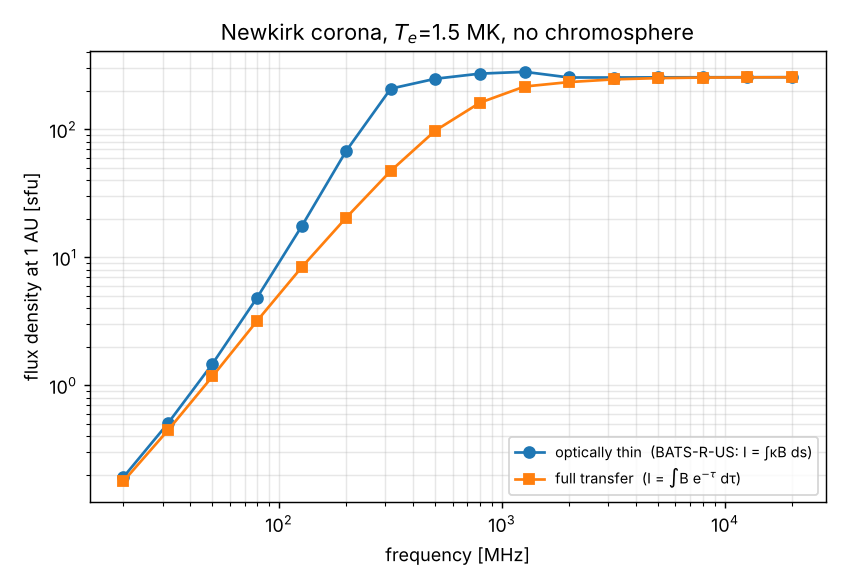
\includegraphics[width=0.62\textwidth]{fig/flux_spectrum.png}
\caption{Flux density at 1\,AU of an isothermal (1.5\,MK) Newkirk corona, optically thin
versus full transfer. The two agree above about 2\,GHz, where the corona is optically
thin.}\label{fig:thinfull}
\end{figure}

\section{BATS-R-US-compatible mode}\label{sec:strict}
By default the step control follows the algorithm as published (Benkevitch et al.\ 2010,
\S5). The Fortran code differs in two ways, and \code{strict\_batsrus=True}
reproduces them exactly:
\begin{enumerate}[itemsep=2pt]
\item The Fortran also applies the parabolic reflection whenever $\Delta s<$
      \code{StepMin} and the ray is moving towards denser plasma. That condition is only
      met after the \emph{curvature} control has reduced the step. It then fires for
      rays far from the critical surface ($\varepsilon\approx0.6$), which jump along a
      long, wrong parabola. In tests on an exact analytic field this caused errors of up
      to 10$^\circ$ in the exit direction, compared with 0.03$^\circ$ without it.
\item The Fortran discards a ray whose mid-point lands in over-dense plasma, keeping only
      the intensity gathered so far. \code{radiosynth} instead steps such a ray back
      with a quarter of the step and, if necessary, reflects it by Snell's law, as both
      papers describe. Head-on rays at the disk centre are then not lost, and the result
      no longer depends on the step size.
\end{enumerate}

%======================================================================
\chapter{Output}
%======================================================================

\section{The \code{RadioImage} object}

\begin{longtable}{@{}p{4.4cm}p{10.8cm}@{}}
\toprule
Attribute / method & Description \\
\midrule\endhead
\code{intensity} & $(n_f,n_y,n_x)$ specific intensity [W\,m$^{-2}$\,Hz$^{-1}$\,sr$^{-1}$] (dimensionless for ``simplistic''). \\
\code{brightness\_temperature} & $T_b=I c^2/(2k_B\nu^2)$ [K] (Rayleigh--Jeans). \\
\code{tau} & Optical depth along each ray (full transfer only; zero otherwise). \\
\code{status} & How each ray ended (Table~\ref{tab:status}). \\
\code{nstep} & Number of integration steps per ray. \\
\code{x}, \code{y} & Pixel-centre coordinates in the image plane [\rsun]. \\
\code{freqs} & Frequencies [Hz]. \\
\code{flux\_density}, \code{flux\_density\_sfu}, \code{flux\_density\_mjy} & Total flux at the observer, $F=\sum I\,\Delta\Omega$, in W\,m$^{-2}$\,Hz$^{-1}$, sfu and mJy. \\
\code{distance}, \code{distance\_pc}, \code{length\_unit} & Observer distance (coordinate units, parsec) and metres per coordinate unit. \\
\code{pixel\_solid\_angle} & $\Delta\Omega=\Delta X\Delta Y/D^2$ [sr]. \\
\code{summary()} & Text summary per frequency. \\
\code{plot(quantity, path, log, ...)} & Image panels of \code{"tb"} or \code{"intensity"}, with the limb drawn. \\
\code{save\_npz(path)} & All arrays and metadata, compressed NumPy. \\
\code{save\_tecplot(path)} & ASCII Tecplot, same layout as BATS-R-US: \code{X Y f=...}. \\
\code{save\_fits(path, quantity)} & FITS cube $(n_f,n_y,n_x)$ of intensity or \code{"tb"}. \\
\code{meta} & Dictionary of the settings used. \\
\bottomrule
\end{longtable}

Array index \code{[k, j, i]} is frequency $k$, image row $j$ ($Y$) and column $i$ ($X$).
With \code{origin="lower"} in \code{imshow} the image appears the right way up.

\begin{table}[h]\centering\small
\begin{tabular}{@{}c l l@{}}
\toprule
Code & Name & Meaning \\
\midrule
1 & escaped & left the model domain or the integration sphere (normal end) \\
2 & hit body & reached the inner boundary $r_\text{body}$ (photosphere) \\
3 & over-dense & entered $n_e\ge n_\text{cr}$ and could not be recovered \\
4 & eps$\le$0 & permittivity at the step start $\le0$ \\
5 & tau$>$tau\_max & full transfer: optically thick, stopped early \\
6 & max steps & stopped by \code{max\_steps} (should not happen) \\
7 & missed grid & the straight ray never enters the model domain \\
\bottomrule
\end{tabular}
\caption{Ray status codes (\code{rs.STATUS\_NAMES}).}\label{tab:status}
\end{table}

\section{Reading saved images}
\begin{lstlisting}[style=pyex]
import numpy as np, matplotlib.pyplot as plt
d = np.load("radio.npz")
tb, x, y, f = d["tb"], d["x"], d["y"], d["freqs"]
plt.imshow(tb[0], origin="lower", extent=[x[0], x[-1], y[0], y[-1]], cmap="inferno")
plt.title(f"{f[0]/1e6:.0f} MHz"); plt.colorbar(label="T_b [K]"); plt.show()
\end{lstlisting}

%======================================================================
\chapter{Command-line reference}
%======================================================================

\begin{lstlisting}
python -m radiosynth INPUT --freq "LIST" [options]
\end{lstlisting}

\begin{longtable}{@{}p{4.6cm}p{10.6cm}@{}}
\toprule
Option & Meaning \\
\midrule\endhead
\code{INPUT} & Model file or PLUTO output directory (see Table~\ref{tab:inputs}). \\
\code{--freq} & Frequency list, e.g.\ \code{"42.3MHz, 125MHz, 17GHz"} (required). \\
\code{--observer X Y Z} & Observer position [\rsun] (default \code{-215 0 0}). \\
\code{--date T}, \code{--frame}, \code{--phi-offset} & Observer at Earth for time \code{T} (\code{carrington} or \code{stonyhurst} model frame, extra longitude offset). \\
\code{--r-star R} & Stellar radius in \rsun; the coordinates are then in stellar radii. \\
\code{--distance-pc D} & Star at \code{D} parsec: parallel rays; the flux density is printed in mJy. \\
\code{--inclination I}, \code{--phase P} & View of a star: inclination of the rotation axis ($z$) and rotational phase [deg]. \\
\code{--size XS YS} & Image size [\rsun] (default \code{6 6}). \\
\code{--npix NX NY} & Pixels (default \code{128 128}). \\
\code{--up X Y Z} & Image up-vector (default \code{0 0 1}). \\
\code{--mechanism} (or \code{--emission}) & \code{bremsstrahlung} | \code{simplistic} | \code{gyroresonance} | \code{gyrosynchrotron} | \code{combined}. \\
\code{--list-mechanisms} & Print the available mechanisms and exit. \\
\code{--gaunt} & Number or \code{dulk} (default 10; \code{dulk} for gyroresonance). \\
\code{--transfer} & \code{thin} | \code{full}. \\
\code{--no-refraction} & Straight lines of sight. \\
\code{--compare-refraction} & Both images (refracted and straight) with a comparison figure; bremsstrahlung and simplistic only. \\
\code{--kappa-over-mu} & Refractive correction to absorption. \\
\code{--r-integration} & Integration-sphere radius [\rsun]. \\
\code{--r-body} & Inner boundary [\rsun] (default 1, or the PLUTO inner radius). \\
\code{--step-factor}, \code{--tolerance} & Accuracy controls. \\
\code{--workers N} & Parallel processes. \\
\multicolumn{2}{@{}l}{\emph{Gyroresonance (\code{--mechanism gyroresonance})}}\\
\code{--gr-mechanisms} & \code{gr+ff} (default) | \code{gr} | \code{ff}. \\
\code{--s-max} & Highest harmonic (default 10). \\
\code{--coupling} & \code{weak} (default) | \code{strong} mode coupling. \\
\code{--ds} & Step along the straight rays [\rsun] (default half the smallest cell). \\
\code{--t-body} & Brightness temperature of the body (e.g.\ \code{1e4}); default none. \\
\code{--b-unit} & Unit of $\vect B$ in the file if not in the variable names: \code{G}, \code{nT}, \code{T} or gauss per unit. \\
\multicolumn{2}{@{}l}{\emph{Gyrosynchrotron (\code{--mechanism gyrosynchrotron}; Chapter~\ref{chap:gs})}}\\
\code{--nb} & Fast-electron density [cm$^{-3}$] (peak of the rule; for \code{thermal-fraction} the fraction). \\
\code{--nb-rule} & \code{sphere} (with \code{--nb-center X Y Z}, \code{--nb-radius}) | \code{uniform} | \code{thermal-fraction} | \code{current} ($n_b\propto|\vect J|$). \\
\code{--delta}, \code{--emin-kev}, \code{--emax-mev} & Power-law index and energy range (default 4, 10\,keV, 10\,MeV). \\
\code{--pitch}, \code{--loss-cone}, \code{--dmu} & Pitch-angle distribution (\code{iso}, \code{gau}, \code{elc}, \code{gab}, \code{sga}), angle, width. \\
\code{--gs-coupling} & \code{exact} (default) | \code{weak} | \code{strong}. \\
\code{--gs-library} & Path of the compiled fast GS codes. \\
\code{--gs-diagnostics} & Also compute free--free alone (map of the fast-electron fraction). \\
\multicolumn{2}{@{}l}{\emph{Combined (\code{--mechanism combined}; Chapter~\ref{chap:combined})}}\\
\code{--include} & Any of \code{ff gr gs} (default all; \code{gs} uses the gyrosynchrotron options above). \\
\code{--ff-refraction} & Correct the free--free part for refraction. \\
\multicolumn{2}{@{}l}{\emph{BATS-R-US / generic input}}\\
\code{--density-var}, \code{--density-unit} & Choose the density variable and its unit (\code{g/cm\^{}3}, \code{kg/m\^{}3}, \code{cm\^{}-3}, \code{m\^{}-3}). \\
\code{--te-var}, \code{--pe-var}, \code{--p-var} & Choose the temperature/pressure variables. \\
\code{--te-const T} & Constant electron temperature [K]. \\
\code{--mu} & $n_e=\rho/(\mu m_p)$ (default 1). \\
\code{--resample N [N N]}, \code{--resample-box}, \code{--resample-method} & Regridding of scattered / AMR points. \\
\code{--save-grid FILE.npz} & Save the $n_e$/$T_e$ grid for fast reuse. \\
\multicolumn{2}{@{}l}{\emph{1D models (Chapter~\ref{chap:sym})}}\\
\code{--profile} & INPUT is a text table of a 1D model. \\
\code{--profile-cols R N [T]} & Columns of radius, density and temperature. \\
\code{--profile-density}, \code{--profile-density-unit} & \code{ne} (cm$^{-3}$, m$^{-3}$) or \code{rho} (g/cm$^3$, kg/m$^3$). \\
\code{--profile-r-unit} & Coordinate units (\rsun{} or $R_\ast$) per file unit of $r$. \\
\code{--symmetric} & One row of rays, rotated; writes the radial profile (bremsstrahlung, simplistic). \\
\code{--n-p} & Number of rays for \code{--symmetric} (default 1000). \\
\multicolumn{2}{@{}l}{\emph{PLUTO input}}\\
\code{--nout}, \code{--pluto-format} & Output number (default last); \code{dbl} or \code{flt}. \\
\code{--definitions} & Path to \code{definitions.h}. \\
\code{--unit-density}, \code{--unit-length}, \code{--unit-velocity} & Code units in cgs. \\
\code{--mu-e}, \code{--mmw} & $n_e=\rho/(\mu_e m_p)$; $T=p\mu m_p/(\rho k_B)$. \\
\code{--pypluto [DIR]} & Read the PLUTO data with pyPLUTO (bundled copy, or the one in \code{DIR}). \\
\multicolumn{2}{@{}l}{\emph{Output}}\\
\code{--out PREFIX} & Output file prefix. \\
\code{--formats} & Any of \code{npz tec fits} (default \code{npz tec}). \\
\code{--plot} & Write \code{PREFIX\_Tb.png} and \code{PREFIX\_I.png} (gyroresonance: also \code{\_pol.png}, \code{\_harmonic.png}; FITS output adds \code{\_V.fits}, \code{\_TbV.fits}). \\
\bottomrule
\end{longtable}

%======================================================================
\chapter{Worked examples}
%======================================================================

\section{Multi-frequency images}
The demonstration script \code{examples/demo.py} builds an analytic corona: a Newkirk
density profile with an equatorial streamer and a dense CME-like blob above the west
limb. It then images the model at six frequencies (Fig.~\ref{fig:multi}).

\begin{lstlisting}[style=pyex]
import sys; sys.path.insert(0, "examples")
import radiosynth as rs
from synthetic_corona import make_model
grid = make_model(half=4.0, n=201, te=1.5e6, streamer=True,
                  blob=((0.3, -1.9, 0.6), 0.45, 4.0))
img = rs.make_radio_image(grid, "42.3MHz, 80MHz, 150MHz, 327MHz, 1GHz, 17GHz",
                          (-215, 0, 0), 8, 8, 128, 128, transfer="full", n_workers=4)
img.plot("tb", path="images_full_Tb.png", log=False, vmin=0)
\end{lstlisting}

\begin{figure}[h]
\centering
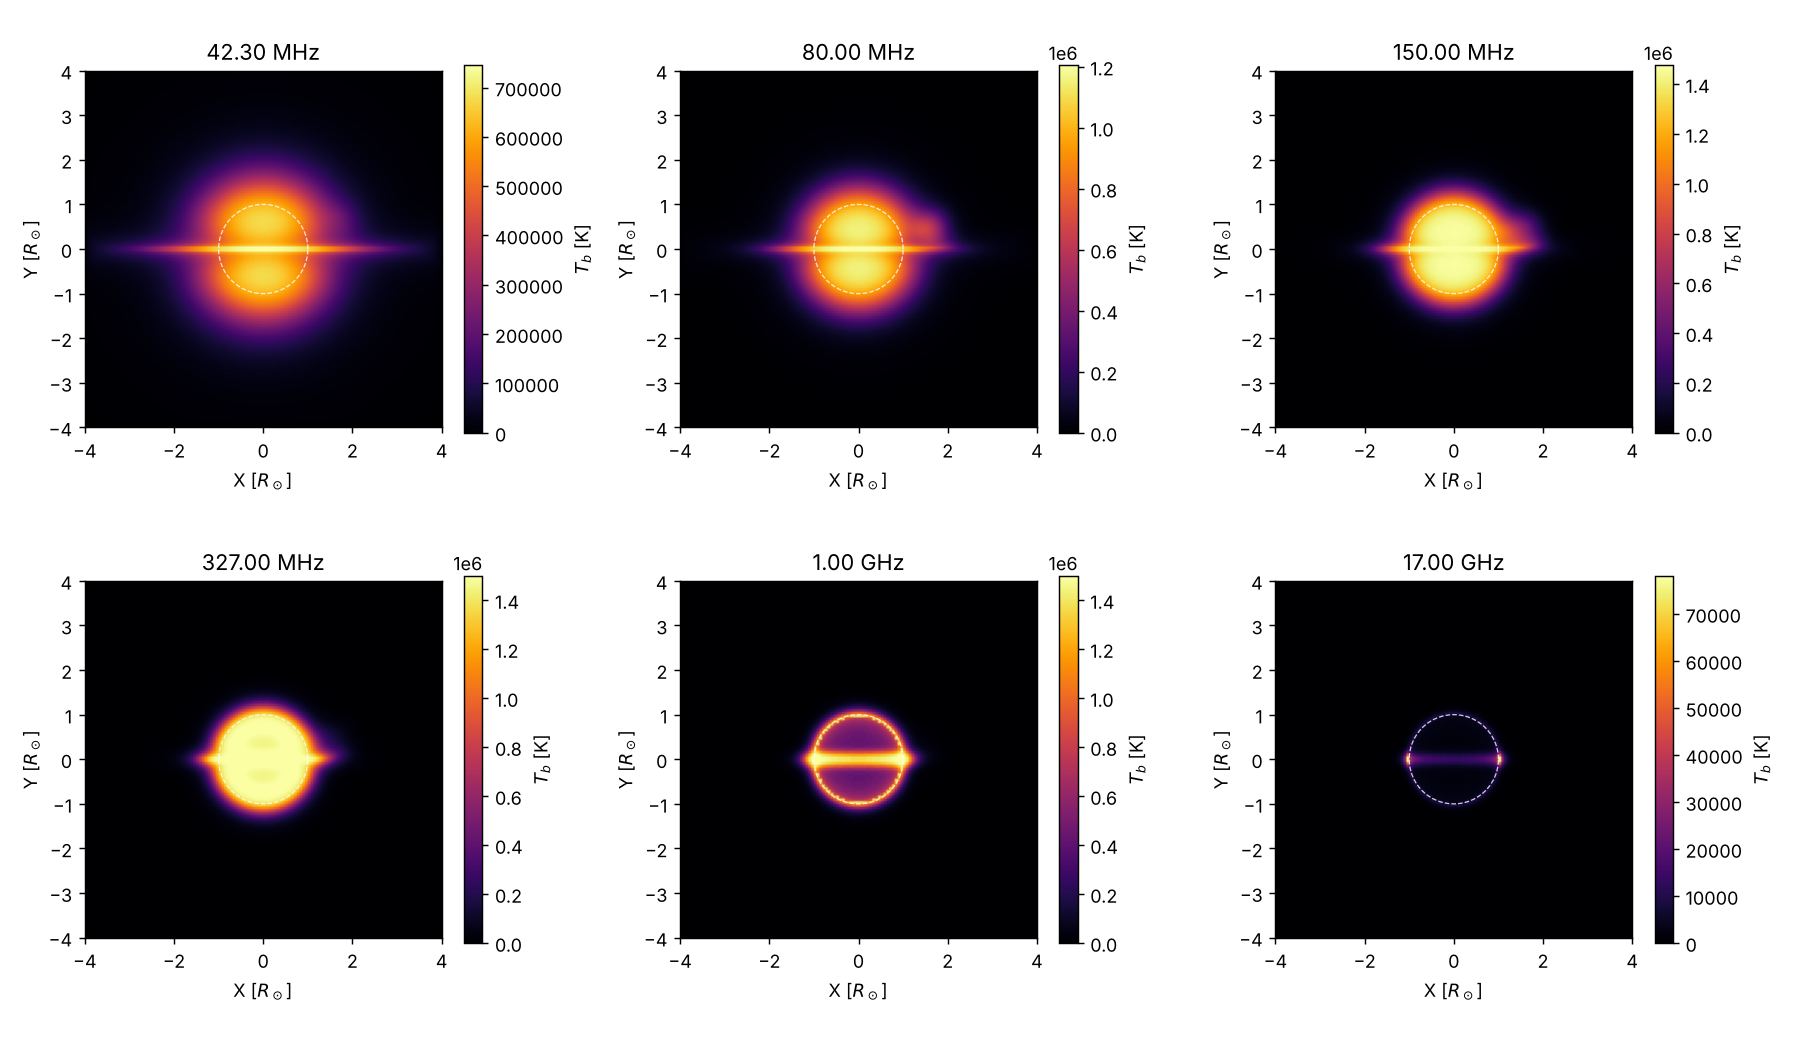
\includegraphics[width=\textwidth]{fig/images_full_Tb.png}
\caption{Brightness temperature (full transfer) of the test corona. At low frequencies
the radio Sun is large and limb-brightened by the streamer, and the CME blob shows up
west of the disk. At high frequencies the purely coronal model becomes optically thin;
a real model would need a chromosphere here.}\label{fig:multi}
\end{figure}

\section{Refracted rays versus straight lines of sight}\label{sec:refcmp}
As in Moschou et al.\ (2018, Fig.~4), compare the image along refracted rays with the
image along straight lines of sight:
\begin{lstlisting}[style=pyex]
ref = rs.make_radio_image(grid, "80MHz", (-215,0,0), 8, 8, 128, 128, n_workers=4)
los = rs.make_radio_image(grid, "80MHz", (-215,0,0), 8, 8, 128, 128, n_workers=4,
                          no_refraction=True)
\end{lstlisting}
Along straight lines of sight a bright ring appears at the edge of the critical surface
(Fig.~\ref{fig:los}), as reported in the paper. With \code{strict\_batsrus=True} the
image is almost the same at this resolution.

\paragraph{One call for the comparison.} \code{compare\_refraction} computes both images
with identical settings (only \code{no\_refraction} differs), reports the flux ratio and
the fraction of emitting pixels that change by more than 10\%, and draws refracted,
straight and their ratio for every frequency (Fig.~\ref{fig:refcmp}):
\begin{lstlisting}[style=pyex]
res = rs.compare_refraction(grid, "80MHz, 17GHz", observer=(-215, 0, 0), x_size=5, y_size=5,
                            nx=128, ny=128, transfer="full", path="refraction.png")
res["refracted"], res["straight"]          # the two RadioImages
res["flux_ratio"], res["changed"]          # per frequency
rs.simplistic.compare_refraction(grid, "80MHz")        # same for the simplistic mechanism
\end{lstlisting}
On the command line: \code{--compare-refraction} (writes \code{PREFIX\_refracted.*},
\code{PREFIX\_straight.*} and \code{PREFIX\_refraction.png}). It is available for the
mechanisms that use the refractive ray tracer (\code{bremsstrahlung}, \code{simplistic},
or your own emission function); the gyroresonance and gyrosynchrotron images are computed
along straight rays only (Chapter~\ref{chap:mech}).

\begin{figure}[h]
\centering
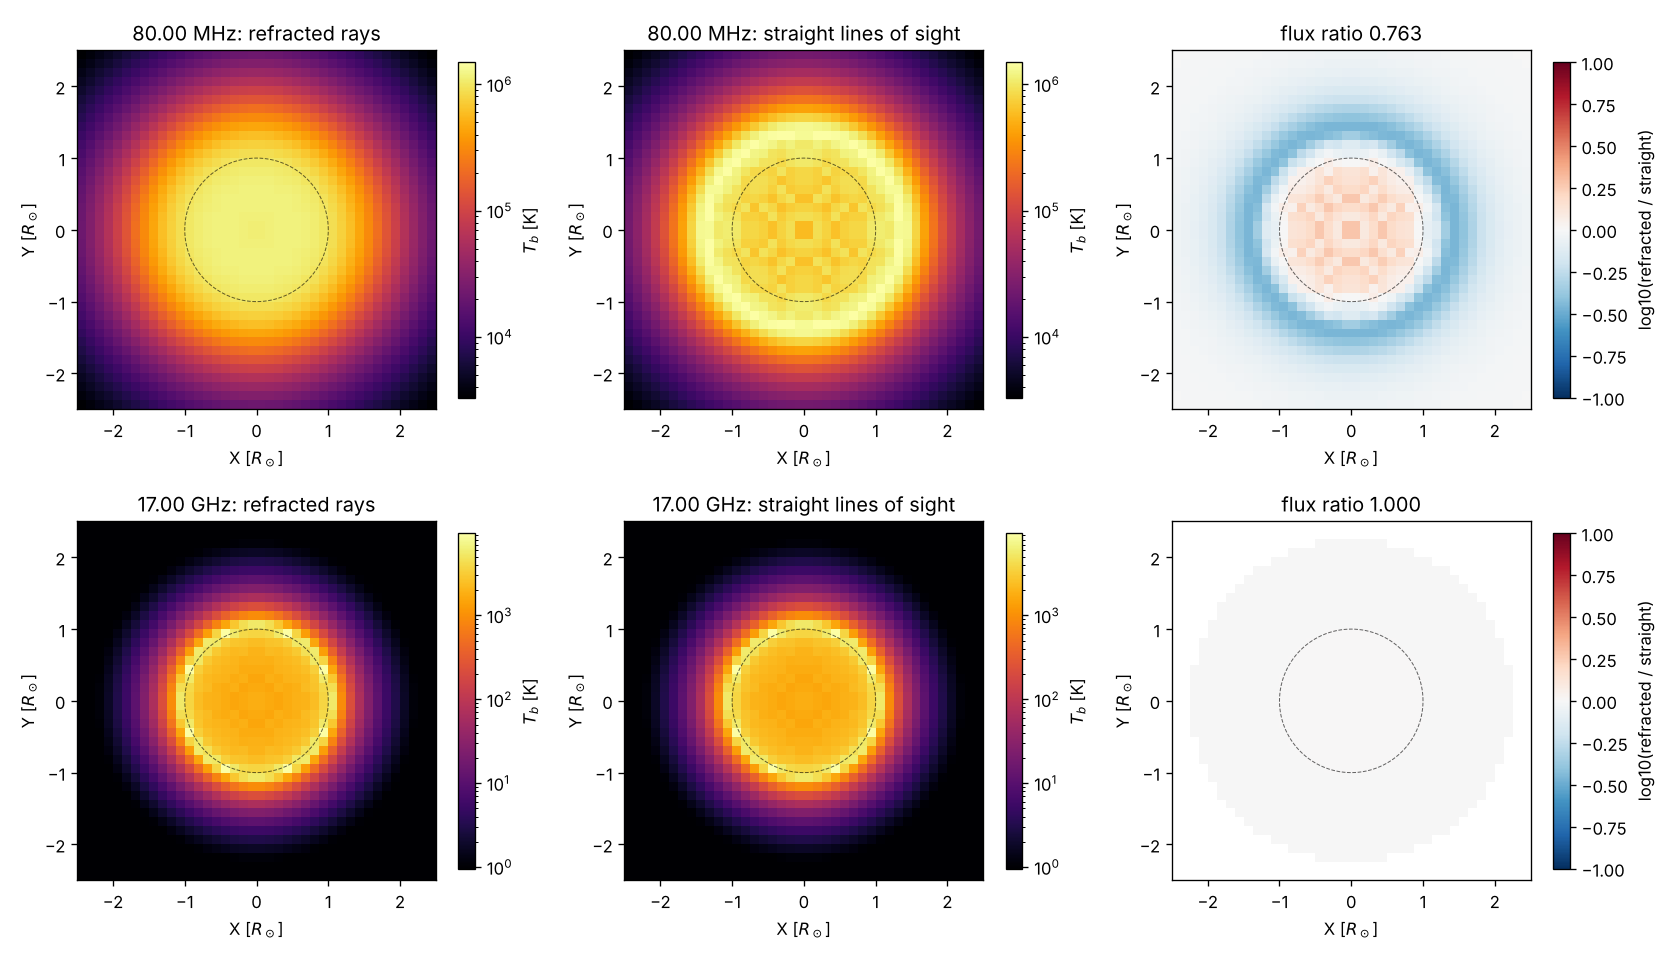
\includegraphics[width=\textwidth]{fig/refraction_compare.png}
\caption{\code{compare\_refraction} on the Newkirk corona (full transfer): at 80\,MHz
refraction removes the bright limb ring of the straight-line image and changes the flux
by 24\%; at 17\,GHz the two images are identical to $2\times10^{-4}$.}\label{fig:refcmp}
\end{figure}

\begin{figure}[h]
\centering
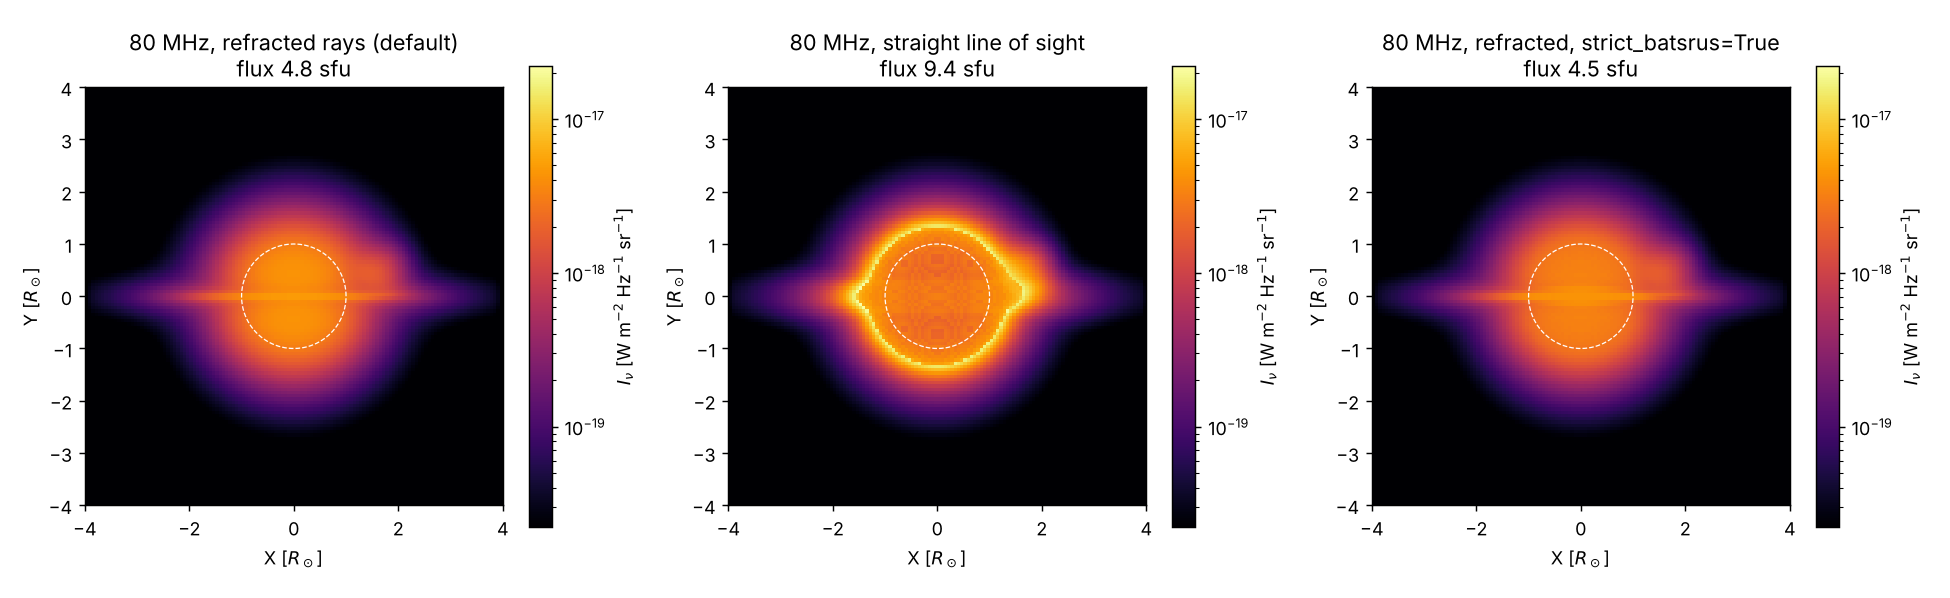
\includegraphics[width=\textwidth]{fig/refraction_vs_los_80MHz.png}
\caption{80\,MHz optically thin intensity: refracted rays (left), straight lines of sight
(middle), and the exact BATS-R-US step logic (right).}\label{fig:los}
\end{figure}

\section{Ray paths}
\code{trace\_paths} returns the trajectories of selected rays, given by their image-plane
coordinates. This is useful for checking where the emission comes from:
\begin{lstlisting}[style=pyex]
import numpy as np, matplotlib.pyplot as plt
yp = np.linspace(-2.4, 2.4, 25)                    # image-plane Y of each ray
r = rs.trace_paths(grid, 80e6, (-215, 0, 0), 0*yp, yp, x_size=6, y_size=6)
for k in range(len(yp)):
    P = r["paths"][k]                               # (M,3) positions, R_sun
    plt.plot(P[:, 0], P[:, 2])
plt.gca().set_aspect("equal"); plt.show()
\end{lstlisting}
The result is shown on the title page and in Fig.~\ref{fig:paths} of Part~II.

\section{Flux-density spectrum}
\begin{lstlisting}[style=pyex]
freqs = np.geomspace(20e6, 20e9, 16)
img = rs.make_radio_image(grid, freqs, (-215,0,0), 8, 8, 64, 64, transfer="full", n_workers=4)
plt.loglog(freqs/1e6, img.flux_density_sfu)
\end{lstlisting}

\section{A user-defined emission mechanism}
Any function returning $(\kappa\,[\text{m}^{-1}], B\,[\text{W m}^{-2}\text{Hz}^{-1}\text{sr}^{-1}])$
can be used, for example a gyroresonance or non-thermal model:
\begin{lstlisting}[style=pyex]
def my_emission(ne, te, freq):
    kappa, B = rs.EmissionModel("bremsstrahlung", gaunt="dulk")(ne, te, freq)
    return 1.5 * kappa, B          # e.g. an enhanced opacity
img = rs.make_radio_image(grid, "150MHz", emission=my_emission, transfer="full")
\end{lstlisting}

\section{A typical PLUTO solar-wind workflow}
\begin{lstlisting}[style=pyex]
import radiosynth as rs
grid = rs.load_pluto("sw_run/out", nout=-1, mu_e=1.17, mean_mol_weight=0.6)
grid.to_npz("sw_grid.npz")                         # optional cache
img = rs.make_radio_image(grid, "80MHz, 150MHz, 240MHz, 327MHz",
                          observer=(-215, 0, 0), x_size=6, y_size=6,
                          nx=256, ny=256, transfer="full", n_workers=8)
img.plot("tb", path="sw_Tb.png", log=False, vmin=0)
img.save_fits("sw_Tb.fits", quantity="tb")
print(img.summary())
\end{lstlisting}

%======================================================================
\chapter{Figures in the style of Moschou et al.\ (2018)}\label{chap:figs}
%======================================================================

The module \code{radiosynth.figures} (\code{rs.figures}) makes figures like those of
Moschou et al.\ (2018). The script \code{examples/moschou\_figures.py} produces all of
them from a test corona with three hot, dense active regions and an expanding
three-part CME. Replace the model and the mock observation with your own data to make
the real figures.

\begin{table}[h]\centering\small
\begin{tabularx}{\textwidth}{@{}l l X@{}}
\toprule
Paper & Function & Content \\
\midrule
Fig.~2 & \code{figure\_compare\_observation} & synthetic map with log contours, next to an observed map (e.g.\ Nobeyama 17\,GHz) with the synthetic contours and the limb overplotted \\
Fig.~3 & \code{figure\_single\_map} & one frequency, rainbow colour map, white log contours, limb, frequency label \\
Fig.~5 & \code{figure\_time\_series} & rows = times, columns = frequencies; common log scale; 10 log-spaced contours; time stamps \\
animations & \code{animate\_time\_series} & GIF or MP4 of one frequency through a time series \\
helpers & \code{make\_time\_series}, \code{earth\_observer}, \code{rsun\_to\_arcsec}, \code{read\_fits\_map}, \code{smooth\_to\_beam} & \\
orientation & \code{observer\_for\_date}, \code{sun\_ephemeris}, \code{fit\_longitude\_offset} & observer at Earth for a date; fit of the model's longitude offset (Section~\ref{sec:orient}) \\
statistics & \code{compare\_with\_observation} & profiles, disk/limb $T_b$, correlation, residuals (Chapter~\ref{chap:plutoobs}) \\
\bottomrule
\end{tabularx}
\end{table}

\section{Coordinates and orientation}
To compare with observations, the synthetic image must have the same orientation and
scale as the observed map.
\begin{itemize}[itemsep=2pt]
\item \textbf{Orientation.} If the model uses a heliographic frame with $z$ along the
      solar rotation axis, as BATS-R-US SC/IH do (HGR, Carrington), place the observer
      with \code{rf.earth\_observer(B0, L0)} and keep \code{up=(0,0,1)}. The image then
      has solar North up and West to the right, like Nobeyama, MWA or LOFAR maps. For an
      HGR (Carrington) model, $L_0$ is the Carrington longitude of the Earth at the time
      of the observation:
\begin{lstlisting}[style=pyex]
obs = rs.figures.observer_for_date("2011-03-07T03:00")       # B0, L0, distance
# equivalent: eph = rs.figures.sun_ephemeris(t); rs.figures.earth_observer(eph["B0"], eph["L0"])
\end{lstlisting}
      For PLUTO and other models without solar coordinates, see
      Section~\ref{sec:orient}.
\item \textbf{Scale.} The image-plane coordinate $X$ [\rsun] corresponds to the
      helioprojective angle $T_x=\arctan(X/D)$. The figure functions do this conversion
      when \code{units="arcsec"}.
\item \textbf{Resolution.} \code{beam\_fwhm\_arcsec} convolves the synthetic map with
      the instrument beam before contouring (about 10'' for NoRH at 17\,GHz, a few
      arcminutes for MWA).
\end{itemize}

\section{Models without solar coordinates (PLUTO and others)}\label{sec:orient}
A PLUTO run has no built-in solar coordinate system. Its axes mean whatever the setup
(\code{init.c}, the boundary data) makes them mean. Before comparing with an observation,
decide which of these cases applies.

\paragraph{1. Data-driven run (magnetogram at the inner boundary).}
If \code{init.c} maps a synoptic magnetogram onto the grid with
$\theta=90^\circ-$latitude and $\phi=$ Carrington longitude, then the model is in the
Carrington frame, like BATS-R-US: $z$ is the rotation axis (solar north) and $\phi=0$ is
Carrington longitude 0. Place the observer for the date of the observation:
\begin{lstlisting}[style=pyex]
obs = rs.figures.observer_for_date("2014-11-01T03:00", phi_offset_deg=0.0)
img = rs.make_radio_image(grid, "125MHz", obs, 4.4, 4.4, 256, 256, up=(0, 0, 1))
\end{lstlisting}
\code{observer\_for\_date} computes $B_0$, the Carrington longitude $L_0$, the
position angle $P$ and the Sun--Earth distance. It uses sunpy if installed, and otherwise
the algorithm of Meeus (\emph{Astronomical Algorithms}, ch.~25 and 29), which agrees with
Meeus' worked example to $0.02^\circ$. The observer is placed at latitude $B_0$ and
longitude $L_0+$\code{phi\_offset\_deg}.

Check three things in your setup:
\begin{itemize}[itemsep=1pt]
\item \textbf{Longitude offset.} Some setups shift the map, for example $\phi=0$ at the
      map's left edge or at its central meridian. Put that shift into
      \code{phi\_offset\_deg}.
\item \textbf{Latitude direction.} If $\theta=0$ is the south pole, use \code{up=(0,0,-1)}.
\item \textbf{Epoch.} $L_0$ changes by about $13.2^\circ$ per day, so use the time of the
      observation.
\end{itemize}

\paragraph{2. Idealised run (dipole, analytic structures).}
There is no ``true'' orientation. Use \code{frame="stonyhurst"} (model longitude 0
faces the Earth) or any \code{earth\_observer(B0, L)}. Compare quantities that do not
depend on the exact orientation, such as disk size against frequency, limb brightening,
$T_b$ and flux spectra.

\paragraph{3. Rotation axis not along $z$.}
Give the two directions in model coordinates:
\code{make\_radio\_image(grid, f, 215*earth\_dir, ..., up=north\_dir)}. The image ``up''
is the projection of \code{north\_dir} onto the sky.

\paragraph{The observation must be solar-north-up as well.}
NoRH maps are normally already in solar coordinates; check the \code{SOLP}/\code{CROTA}
keywords. MWA and LOFAR images often come in RA/Dec and must first be rotated by the
P-angle. The P-angle is printed by \code{observer\_for\_date}; with sunpy, use
\code{sunpy.map.Map(f).rotate()}.

\paragraph{Unknown longitude offset: fit it.}
If the offset of a data-driven run is uncertain, find it from the data.
\code{fit\_longitude\_offset} computes a synthetic map for each trial offset. It smooths
each map to the beam, interpolates it onto the observed pixels, and correlates the
logarithms inside $r<1.1$ apparent solar radii. The best offset is then refined with a
parabola.
\begin{lstlisting}[style=pyex]
eph = rs.figures.sun_ephemeris("2011-03-07T03:00")
res = rs.figures.fit_longitude_offset(grid, "norh_17GHz.fits", "17GHz",
                                      eph["B0"], eph["L0"], offsets=range(-60, 61, 5),
                                      beam_fwhm_arcsec=10, npix=128, n_workers=8,
                                      plot_path="lonfit.png")
off = res["best_refined"]             # use it for every other frequency / time:
obs = rs.figures.observer_for_date("2011-03-07T03:00", phi_offset_deg=off)
\end{lstlisting}
Use a high frequency (e.g.\ 17\,GHz) for the fit. There refraction is small and compact
active regions dominate the match. You can then refine with a finer grid of offsets around
the best value. In the test (\code{tests/test\_orientation.py}) a mock observation made
with a known offset of $+17^\circ$ was recovered as $+16.8^\circ$
(Fig.~\ref{fig:lonfit}).

\begin{figure}[h]\centering
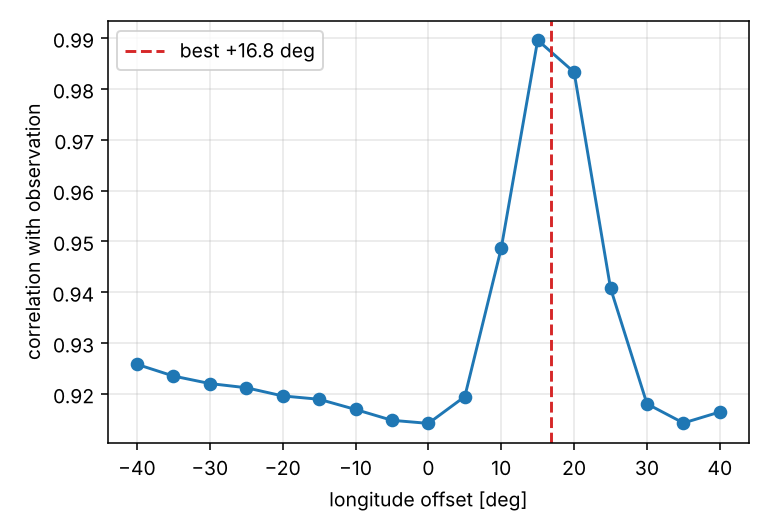
\includegraphics[width=0.55\textwidth]{fig/lonfit_17.png}
\caption{Correlation of synthetic 17\,GHz maps with a mock observation made with a
$+17^\circ$ offset, as a function of the trial longitude offset.}\label{fig:lonfit}
\end{figure}

From the command line, \code{--date} replaces \code{--observer}:
\begin{lstlisting}
python -m radiosynth run/out --freq "125MHz" --date 2014-11-01T03:00 --phi-offset 12.5 --plot
\end{lstlisting}

\section{Single-frequency map (Fig.~3)}
\begin{lstlisting}[style=pyex]
import radiosynth as rs
from radiosynth import figures as rf
grid = rs.load_pluto("run/out")                         # or rs.load_mhd(...)
img = rs.make_radio_image(grid, "125MHz", rf.earth_observer(B0, L0), 4.4, 4.4, 256, 256,
                          n_workers=8)
rf.figure_single_map(img, "125MHz", units="arcsec", cmap="jet", n_contours=8,
                     contour_decades=3, path="fig3_125MHz.png")
\end{lstlisting}
\begin{figure}[h]\centering
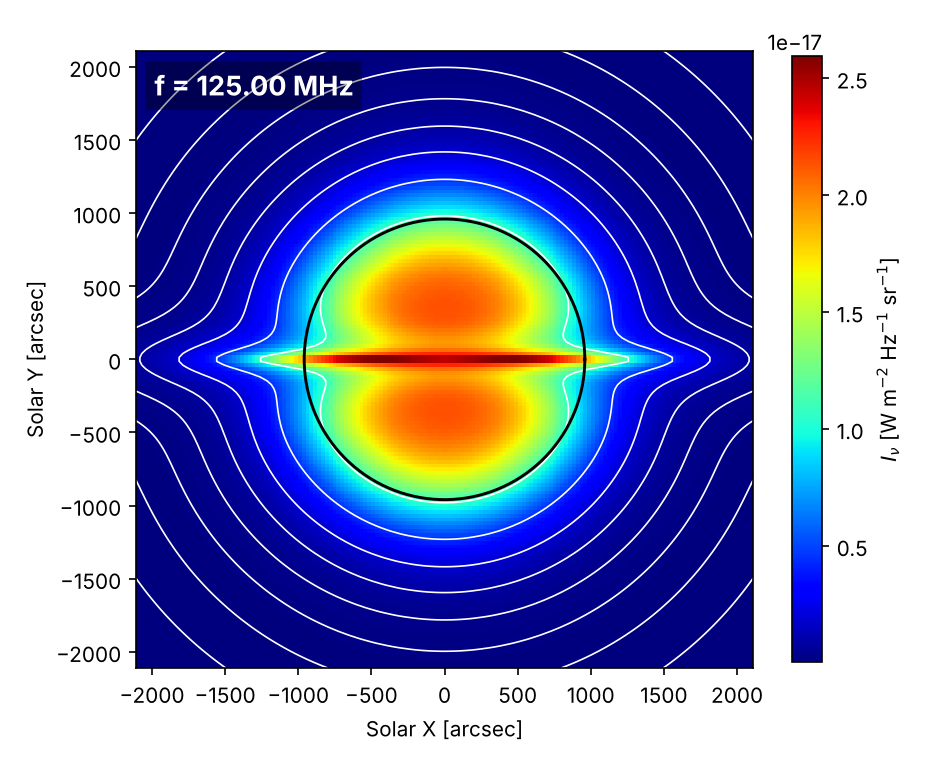
\includegraphics[width=0.62\textwidth]{fig/moschou_fig3_125MHz.png}
\caption{Fig.~3 style: 125\,MHz optically thin intensity of the test corona.}
\end{figure}

\section{Synthetic map versus observation (Fig.~2)}
\begin{lstlisting}[style=pyex]
img = rs.make_radio_image(grid, "17GHz", rf.earth_observer(B0, L0), 2.6, 2.6, 300, 300,
                          n_workers=8)
rf.figure_compare_observation(img, "ipa110307_0300.fits",       # e.g. a NoRH 17 GHz map
                              freq="17GHz", beam_fwhm_arcsec=10, levels="decades",
                              obs_label="NoRH 17 GHz", fov_arcsec=1250,
                              path="fig2_17GHz.png")
\end{lstlisting}
The observation can be a FITS file (helioprojective arcsec, solar North up; a
\code{CROTA2} rotation is corrected) or an array plus its extent
\code{obs\_extent=[Tx0, Tx1, Ty0, Ty1]}. For maps in other projections, use
\code{sunpy.map.Map(file).rotate()} and pass \code{(m.data, extent)}.

\begin{figure}[h]\centering
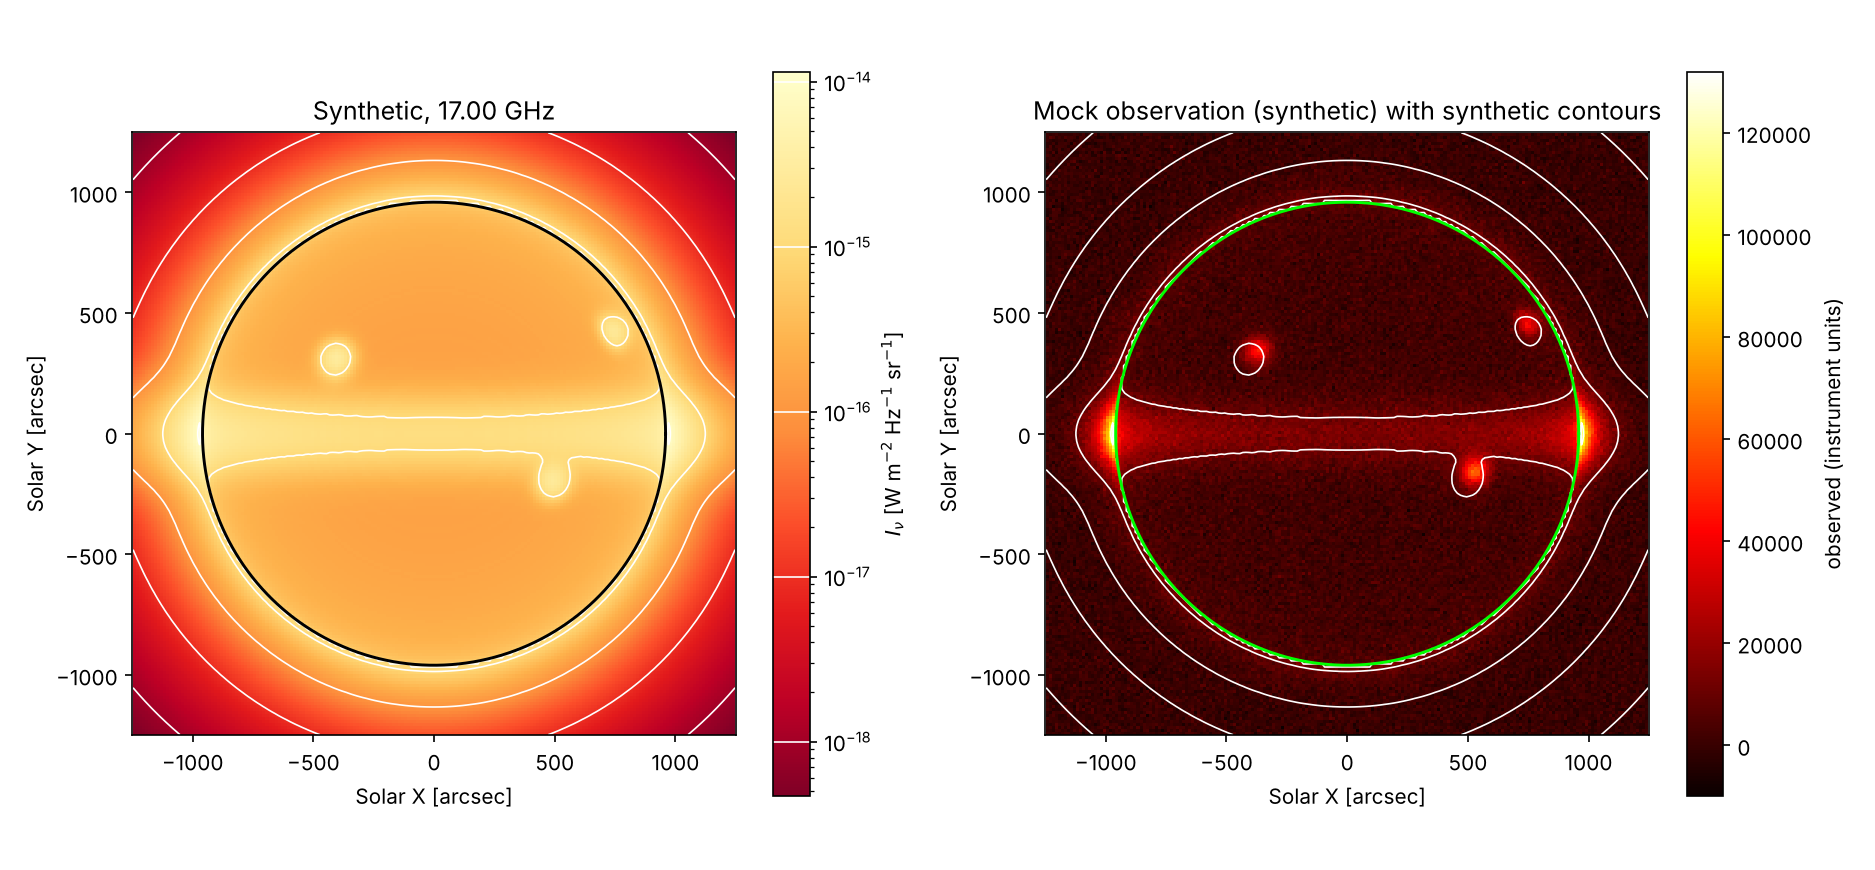
\includegraphics[width=\textwidth]{fig/moschou_fig2_17GHz.png}
\caption{Fig.~2 style. Left: synthetic 17\,GHz intensity with one contour per decade.
Right: a \emph{mock} observation with the synthetic contours. The mock observation is a
perturbed model, smoothed to a 10'' beam and with noise added, written to FITS; it is
\emph{not} real data. It only stands in for a Nobeyama map to show the workflow.}
\end{figure}

\section{CME time series (Fig.~5) and animations}
\begin{lstlisting}[style=pyex]
snaps = ["run/out_t10", "run/out_t38"]                 # PLUTO directories / BATS-R-US files
imgs = rf.make_time_series(snaps, "125MHz, 250MHz, 300MHz, 500MHz", obs, 8, 8, 256, 256,
                           n_workers=8, save_prefix="cme")   # cme_000.npz, cme_001.npz
rf.figure_time_series(imgs, times=[10, 38], n_contours=10, contour_decades=5,
                      fov=3.5, cmap="afmhot", path="fig5_cme.png")
# animation of one frequency through many snapshots
many = rf.make_time_series(sorted(glob.glob("run/out_*")), "125MHz", obs, 8, 8, 128, 128)
rf.animate_time_series(many, "cme_125MHz.gif", times=t_list, fps=4)   # or .mp4
\end{lstlisting}
For PLUTO runs that write all outputs to one directory, use a loader:
\code{make\_time\_series(range(10, 40), ..., loader=lambda n: rs.load\_pluto("run/out", nout=n))}
(any list of items works when \code{loader} is given).

\begin{figure}[h]\centering
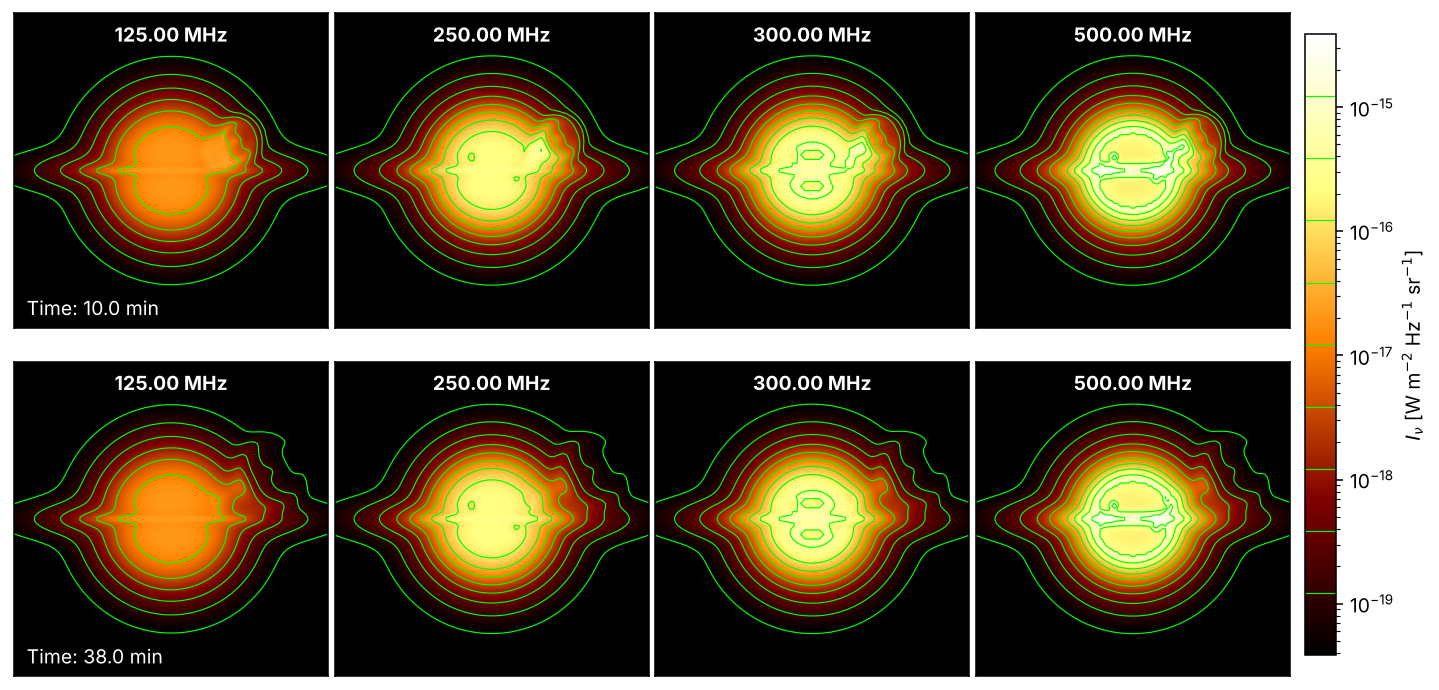
\includegraphics[width=\textwidth]{fig/moschou_fig5_cme.png}
\caption{Fig.~5 style: test-corona CME at 125, 250, 300 and 500\,MHz, 10 and 38\,min
after onset, with 10 logarithmically spaced contours on a common scale.}
\end{figure}

%======================================================================
\chapter{Comparing PLUTO output with observations}\label{chap:plutoobs}
%======================================================================

This chapter goes step by step from a PLUTO run to a quantitative comparison with an
observed radio map, for example Nobeyama (17/34\,GHz), MWA (80--300\,MHz), LOFAR
(30--240\,MHz) or the GRH/VLA. The same steps apply to any MHD model.

\section*{Step 1 --- Load the run with the right physical units}
\begin{lstlisting}[style=pyex]
import radiosynth as rs
from radiosynth import figures as rf
grid = rs.load_pluto("run/out", nout=40,                 # or reader="pypluto"
                     definitions="run/definitions.h",    # UNIT_DENSITY, UNIT_LENGTH, UNIT_VELOCITY
                     mu_e=1.17, mean_mol_weight=0.6)     # the composition used in the run
grid.to_npz("run_n40.npz")                               # fast reload: rs.load_mhd("run_n40.npz")
\end{lstlisting}
Check the printed inner radius (about 1\,\rsun) and the typical $n_e$ and $T_e$ at
$r\approx1.1\,\rsun$. You should see $n_e\sim10^{14}$--$10^{15}$\,m$^{-3}$ and
$T_e\sim1$--2\,MK. If the run evolves only a polytropic or isothermal energy equation,
the temperature from $p/\rho$ may be unrealistic; use \code{te\_const} or replace $T_e$
(Step~8).

\section*{Step 2 --- Fix the orientation of the model}
As explained in Section~\ref{sec:orient}:
\begin{itemize}[itemsep=1pt]
\item \textbf{Data-driven run in Carrington coordinates}:
      \code{obs = rf.observer\_for\_date(t\_obs, phi\_offset\_deg=...)}, with \code{up=(0,0,1)}.
\item \textbf{Idealised run}: choose a viewing direction, e.g.\
      \code{rf.earth\_observer(B0, 0)}, and compare orientation-independent quantities only.
\item \textbf{Uncertain longitude offset}: fit it once with
      \code{rf.fit\_longitude\_offset} at a high frequency, then keep it fixed.
\end{itemize}

\section*{Step 3 --- Prepare the observation}
\begin{itemize}[itemsep=2pt]
\item \textbf{Coordinates.} You need a 2D map in helioprojective arcsec with solar north
      up. NoRH maps normally are. MWA and LOFAR maps are often in RA/Dec: rotate them by
      the P-angle (printed by \code{observer\_for\_date}) or use
      \code{sunpy.map.Map(f).rotate()}.
\item \textbf{Units.} Convert to brightness temperature [K] if possible; many pipelines
      deliver $T_b$ directly. Interferometric images (MWA, LOFAR) often have an uncertain
      absolute scale and miss the large-scale flux. For those, compare morphology and
      relative brightness rather than absolute $T_b$, or compare the total flux with a
      calibrated spectrum.
\item \textbf{Beam.} Note the beam size (FWHM) and pass it as \code{beam\_fwhm\_arcsec}.
      For an elliptical beam, use the geometric mean of the axes or smooth the synthetic
      map yourself.
\item \textbf{Time.} Use the observation time for \code{observer\_for\_date}. If the run
      was driven by a synoptic map, it describes a rotation-averaged corona.
\end{itemize}

\section*{Step 4 --- Compute the synthetic map at the observed frequency}
\begin{lstlisting}[style=pyex]
obs = rf.observer_for_date("2014-11-01T03:00", phi_offset_deg=0.0)
img = rs.make_radio_image(grid, "120MHz", obs,
                          x_size=6.0, y_size=6.0, nx=256, ny=256,   # cover the observed FOV
                          transfer="full",                           # physical T_b (<= T_e)
                          n_workers=8)
img.save_npz("syn_120MHz.npz"); img.save_fits("syn_120MHz_Tb.fits", quantity="tb")
\end{lstlisting}
\begin{itemize}[itemsep=1pt]
\item Use \code{transfer="full"} to compare brightness temperatures. The optically thin
      BATS-R-US mode overestimates $T_b$ below about 1\,GHz (Section~\ref{sec:transfer}).
\item Make the pixel size equal to or smaller than the observed pixel size, and the
      field of view at least as large as the observed one.
\item Make sure the model extends far enough: below about 100\,MHz the radio Sun extends
      to 2--3\,\rsun, so the model domain must reach well beyond that.
\end{itemize}

\section*{Step 5 --- Visual comparison}
\begin{lstlisting}[style=pyex]
rf.figure_compare_observation(img, "mwa_120MHz_northup.fits", quantity="tb",
                              beam_fwhm_arcsec=180, levels="log", n_contours=8,
                              obs_label="MWA 120 MHz", fov_arcsec=2500,
                              path="compare_120MHz.png")
\end{lstlisting}
The synthetic contours are drawn on the observation. Check the size of the radio disk,
the positions of bright and dark features (streamers, coronal holes, active regions), and
the limb brightening.

\section*{Step 6 --- Quantitative comparison}
\code{compare\_with\_observation} smooths the synthetic map to the beam, interpolates it
onto the observed pixels, and computes the main statistics:
\begin{lstlisting}[style=pyex]
cmp = rf.compare_with_observation(img, "mwa_120MHz_northup.fits", freq="120MHz",
                                  quantity="tb", beam_fwhm_arcsec=180,
                                  plot_path="compare_120MHz_stats.png")
print(cmp["mean_disk_obs"], cmp["mean_disk_syn"], cmp["ratio_disk"])   # disk T_b
print(cmp["corr_log"])                                                 # morphology
print(cmp["r_half_obs"], cmp["r_half_syn"])                            # size of the radio Sun
# cmp["syn"], cmp["obs"] : both maps on the observed pixels, for your own statistics
# cmp["r_bins"], cmp["prof_obs"], cmp["prof_syn"] : radial profiles
\end{lstlisting}
The optional plot shows both radial profiles and the residual map (synthetic minus
observed).

Useful measures:
\begin{itemize}[itemsep=1pt]
\item the mean $T_b$ of the disk and of the limb (\code{mean\_disk\_*}, \code{mean\_limb\_*});
\item the correlation coefficient of the logarithms (\code{corr\_log}) and the residual map;
\item radial $T_b$ profiles, and the radius where $T_b$ falls to half its maximum
      (\code{r\_half\_*}, the size of the radio Sun);
\item the total flux \code{img.flux\_density\_sfu} against the observed flux or a
      calibrated spectrum (radio-telescope patrols, NoRP);
\item the shift of features between the refracted and the straight-line images
      (\code{no\_refraction=True}), which shows how much refraction matters at that
      frequency.
\end{itemize}

\section*{Step 7 --- Several frequencies and times}
\begin{lstlisting}[style=pyex]
imgs = rf.make_time_series(range(30, 46, 2), "80MHz, 120MHz, 160MHz, 240MHz", obs, 6, 6, 256, 256,
                           loader=lambda n: rs.load_pluto("run/out", nout=n),
                           transfer="full", n_workers=8, save_prefix="pluto_ts")
rf.figure_time_series(imgs, times=list(range(30, 46, 2)), quantity="tb", path="ts.png")
\end{lstlisting}
Compare the frequency dependence of the disk size and the flux spectrum
(\code{img.flux\_density\_sfu} for each frequency) with the observations.

\section*{Step 7b --- 2.5D (axisymmetric) runs: what can be compared?}
A 2.5D PLUTO run in $(r,\theta)$ is read by \code{radiosynth} as a \emph{body of
revolution}: every longitude has the same density and temperature. The ray tracing is
fully 3D through this structure; the test in Chapter~\ref{chap:validation} reproduces
the flux of the equivalent 3D model to 1.4\%. A 2.5D run is therefore a valid model of
the radio Sun, but only of an axisymmetric Sun, and that sets what can be compared.

\begin{center}\small
\begin{tabularx}{\textwidth}{@{}X X@{}}
\toprule
\textbf{Meaningful with 2.5D} & \textbf{Not meaningful with 2.5D} \\
\midrule
Size of the radio Sun against frequency (\code{r\_half}) &
  Individual active regions, coronal holes or streamers at particular longitudes \\
Equator--pole asymmetry: elongation of the radio Sun along the streamer belt
  (\code{elongation}, sector profiles) &
  Pixel-by-pixel maps and correlation coefficients \\
Radial $T_b$ profiles along the equator and over the poles &
  Longitude fits (\code{fit\_longitude\_offset} has nothing to fit) \\
Disk-centre and limb $T_b$; flux-density spectrum &
  CMEs: a 2.5D flux rope is a ring around the axis, which is far too much material \\
Effect of refraction and optical depth with frequency & Time variability due to rotation \\
\bottomrule
\end{tabularx}
\end{center}

Practical rules:
\begin{itemize}[itemsep=2pt]
\item \textbf{Choose matching observations.} Compare with periods when the real corona is
      close to axisymmetric: solar minimum (e.g.\ 2008--2009, 2018--2020), with polar
      coronal holes and a flat equatorial streamer belt and without large active regions.
      Avoid days with bursts or noise storms.
\item \textbf{Orientation.} Only the tilt matters. Use the observation's $B_0$ (from
      \code{sun\_ephemeris}) with any longitude: \code{rf.earth\_observer(B0, 0)}. The
      observed map must be solar-north-up (P-angle corrected). If the symmetry axis of the
      run is meant to be the magnetic axis and that axis is tilted with respect to the
      rotation axis, set \code{up} to the projected direction of the magnetic axis.
\item \textbf{Measures.} Use \code{compare\_with\_observation}. The sector profiles
      (N, E, S, W, $\pm30^\circ$ in position angle by default; change
      \code{sector\_halfwidth}) and the elongation (equatorial/polar size) are the main
      results. Also use the azimuthally averaged profile, \code{r\_half}, and the mean disk
      and limb $T_b$. Compare these at several frequencies, because the elongation and the
      size change with frequency as the critical layer moves outward.
\end{itemize}
\begin{lstlisting}[style=pyex]
g2d = rs.load_pluto("run2d/out", nout=100)                    # axisymmetric (r, theta)
eph = rf.sun_ephemeris("2019-04-10T03:00")
img = rs.make_radio_image(g2d, "80MHz, 120MHz, 160MHz", rf.earth_observer(eph["B0"], 0.0),
                          6, 6, 192, 192, transfer="full", n_workers=8)
for f, fits_file in [("80MHz", "obs80.fits"), ("120MHz", "obs120.fits"), ("160MHz", "obs160.fits")]:
    c = rf.compare_with_observation(img, fits_file, freq=f, beam_fwhm_arcsec=200,
                                    plot_path=f"cmp_{f}.png")
    print(f, "size obs/syn", c["r_half_obs"], c["r_half_syn"],
          " elongation obs/syn", c["elongation_obs"], c["elongation_syn"])
\end{lstlisting}

\begin{figure}[h]\centering
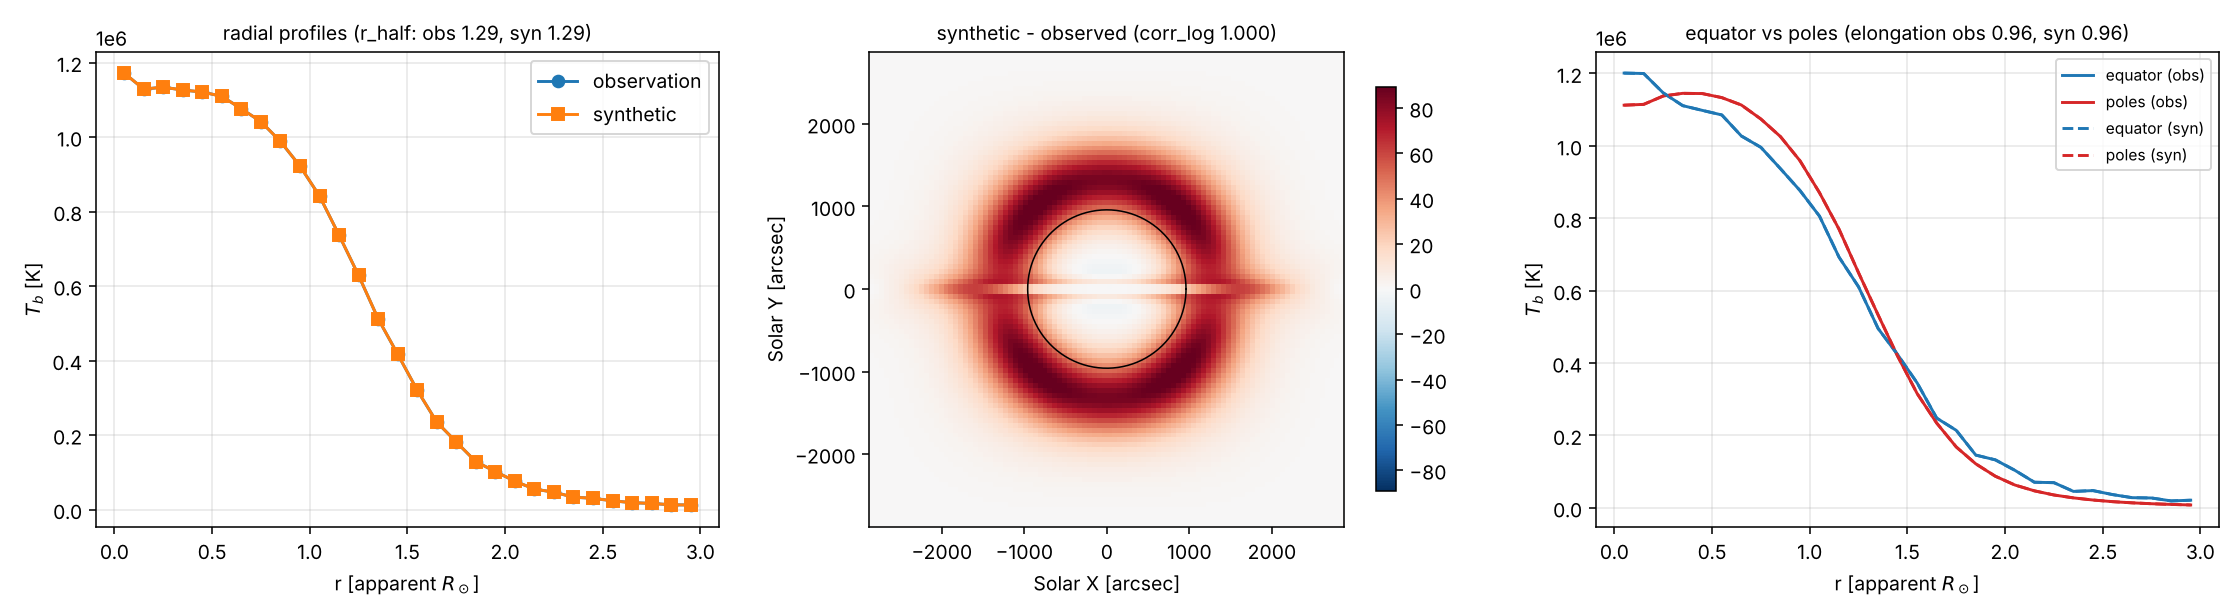
\includegraphics[width=\textwidth]{fig/compare_2p5d.png}
\caption{Output of \code{compare\_with\_observation} for the 2.5D test run at 80\,MHz
(compared with itself, so the curves coincide). Left: azimuthally averaged $T_b$ profile.
Middle: residual map. Right: equatorial and polar profiles. In this test model the
streamer is narrow ($\pm9^\circ$) and there are no polar coronal holes, so the elongation
is close to 1. Solar-minimum observations at metre wavelengths show a radio Sun elongated
along the equator.}
\end{figure}

\section*{Step 8 --- Interpreting differences}
\begin{itemize}[itemsep=2pt]
\item \textbf{Scattering} by density turbulence is not modelled. Below about 200\,MHz it
      makes observed sources larger and the disk dimmer than the synthetic one, so expect
      larger observed sizes at low frequencies (Moschou et al.\ 2018, \S3.3).
\item \textbf{Non-thermal emission} (type I noise storms, bursts, gyro-synchrotron) is not
      included. Remove periods with bursts from the observations.
\item \textbf{Temperature.} A polytropic run with $\gamma\approx1.05$ may give an
      unrealistic $T_e$. Test the sensitivity with \code{te\_const}, or build the grid
      yourself with a temperature model:
      \code{rs.SphericalGrid(g.r, g.theta, g.phi, ne, te\_model, ...)}.
\item \textbf{Lower atmosphere.} At GHz frequencies the emission comes from the
      chromosphere and transition region. If the run starts at the coronal base, the disk
      at these frequencies is too faint.
\item \textbf{Boundary data.} A synoptic magnetogram averages over a whole rotation, so
      small or fast-changing features are not expected to match in detail.
\end{itemize}

%======================================================================
\chapter{Stellar radio emission}\label{chap:stellar}
%======================================================================

The same tracer works for the coronae and winds of other stars. Moschou et al.\ (2018) built
the BATS-R-US tool with stellar applications in mind, and stellar BATS-R-US/AWSoM and PLUTO
wind models can be used directly. Three things differ from the solar case.

\begin{enumerate}[itemsep=2pt]
\item \textbf{Length unit.} Stellar models are written in units of the stellar radius.
      Pass the stellar radius in \rsun{} as \code{r\_star}: the coordinates are then read
      as stellar radii, and every path length is converted with
      $R_\ast=r_\text{star}R_\odot$. This is stored in \code{grid.length\_unit}.
\item \textbf{Distant observer.} A star is seen from parsecs away, so the rays are
      parallel. Give \code{distance\_pc}; the flux density is then computed for that
      distance (\code{img.flux\_density\_mjy}).
\item \textbf{Viewing geometry.} The view is set by the inclination $i$ of the rotation
      axis ($z$) to the line of sight and the rotational phase $\phi$ (the model longitude
      facing the observer): $\hat n=(\sin i\cos\phi,\ \sin i\sin\phi,\ \cos i)$.
\end{enumerate}

\section{Loading a stellar model}
\begin{lstlisting}[style=pyex]
import radiosynth as rs
from radiosynth import stellar as st
# BATS-R-US / AWSoM stellar run (#STAR): coordinates in R_star
grid = rs.load_mhd("3d__mhd_box.dat", r_star=0.42)          # e.g. an M dwarf, 0.42 R_sun
# PLUTO wind/corona with UNIT_LENGTH = R_star (or any unit; it is converted)
grid = rs.load_pluto("wind/out", r_star=0.42)
# your own arrays: coordinates in R_star, n_e [m^-3], T_e [K]
grid = rs.MHDGrid(x, y, z, ne, te, length_unit=0.42 * rs.R_SUN)
\end{lstlisting}
As for the Sun, check the printed $n_e$ and $T_e$. Active stars have much denser and hotter
coronae ($n_e\sim10^{15}$--$10^{17}$\,m$^{-3}$, $T_e\sim3$--30\,MK), so the critical
surface for a given frequency lies further out.

\section{Images, spectra and rotational modulation}
\begin{lstlisting}[style=pyex]
# image of the star at 10 pc, inclination 70 deg, phase 0; field of view 12 R_star
img = st.make_stellar_image(grid, "1.4GHz, 5GHz, 15GHz", inclination_deg=70, phase_deg=0,
                            distance_pc=10, fov=12, npix=160, gaunt="dulk", n_workers=8)
print(img.flux_density_mjy)                                 # mJy at each frequency
rs.figures.figure_single_map(img, "5GHz", quantity="tb", units="mas", cmap="inferno",
                             path="star_5GHz.png")           # VLBI scale: milliarcsec

# spectrum and spectral index S ~ nu^alpha
sp = st.stellar_spectrum(grid, np.geomspace(0.5e9, 50e9, 12), inclination_deg=70,
                         distance_pc=10, fov=15, gaunt="dulk", plot_path="spectrum.png")
sp["freqs"], sp["flux_mjy"], sp["nu_mid"], sp["alpha"]

# rotational modulation (light curve)
lc = st.rotational_modulation(grid, "5GHz", range(0, 360, 20), inclination_deg=70,
                              distance_pc=10, fov=12, plot_path="rotation.png")
\end{lstlisting}
From the command line:
\begin{lstlisting}
python -m radiosynth star_box.dat --r-star 0.42 --distance-pc 10 --inclination 70 \
       --phase 0 --size 12 12 --npix 160 160 --freq "1.4GHz, 5GHz, 15GHz" \
       --transfer full --gaunt dulk --plot
\end{lstlisting}

\begin{figure}[h]\centering
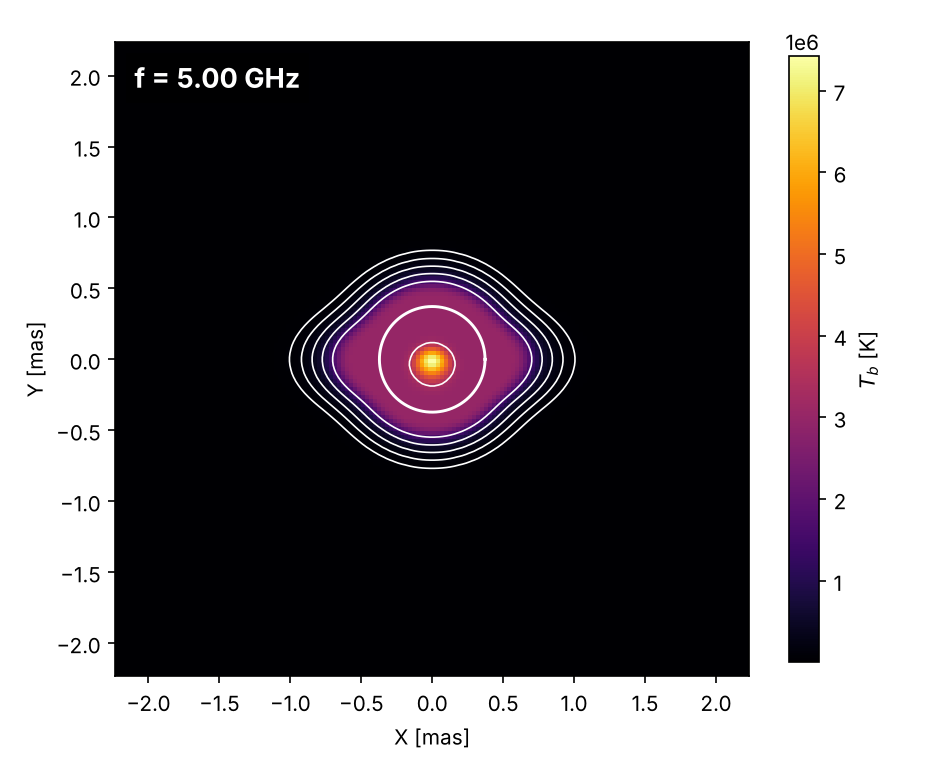
\includegraphics[width=0.48\textwidth]{fig/stellar_image_5GHz.png}\hfill
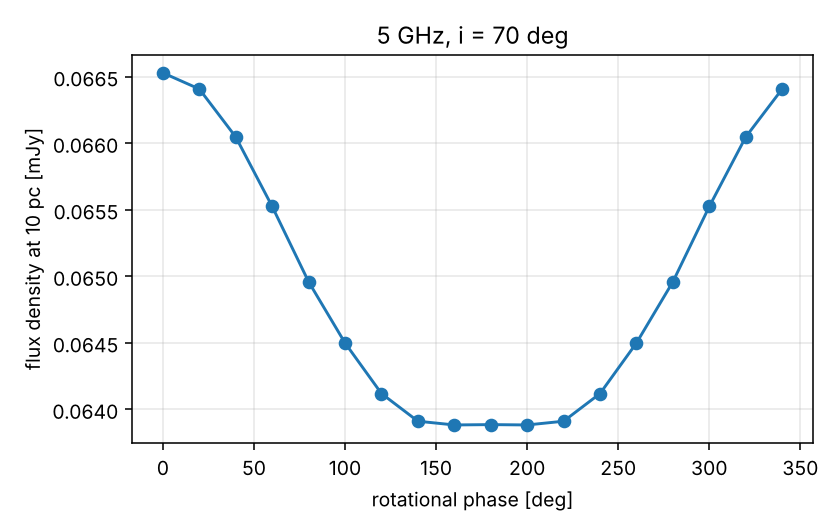
\includegraphics[width=0.48\textwidth]{fig/stellar_example_rotation.png}\\[4pt]
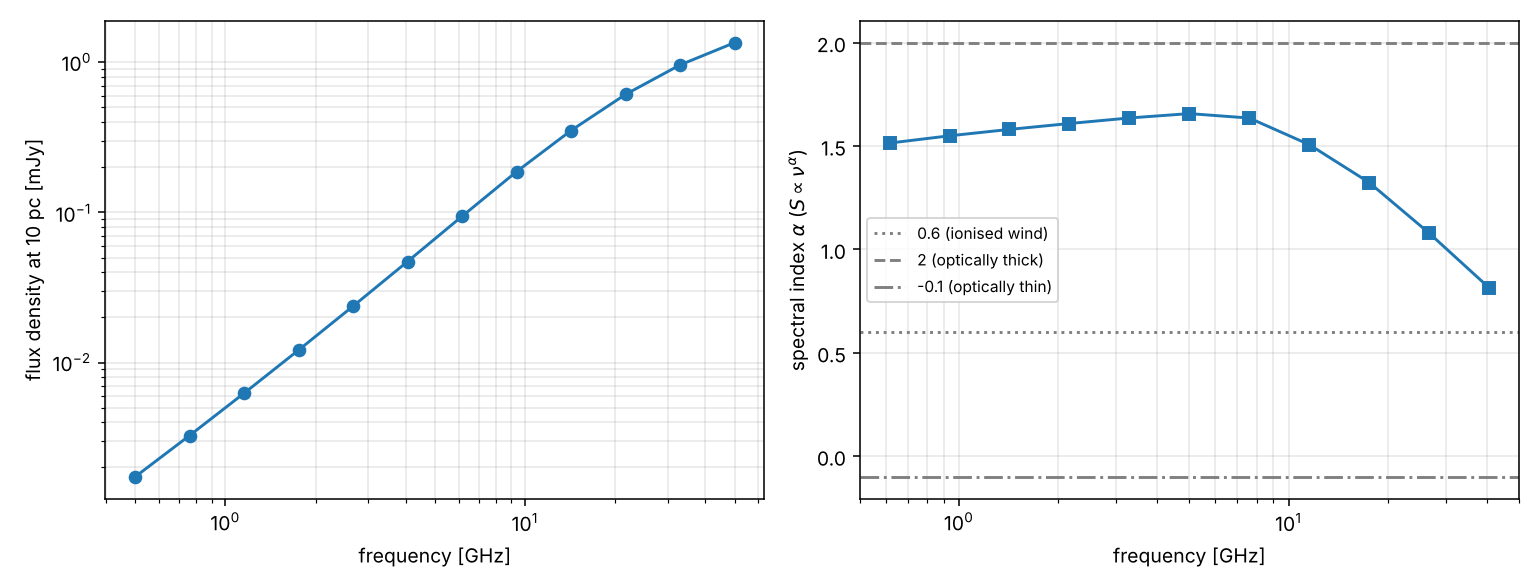
\includegraphics[width=0.9\textwidth]{fig/stellar_example_spectrum.png}
\caption{\code{examples/stellar\_example.py}: an active star ($R_\ast=0.8\,R_\odot$, 3\,MK
corona, a 15\,MK active region, streamer belt and wind) at 10\,pc. Top left: 5\,GHz $T_b$ in
milliarcseconds; the white circle is the photosphere (0.37\,mas). Top right: rotational
modulation at 5\,GHz. Bottom: spectrum and spectral index (Dulk Gaunt factor). The
partially optically thick corona gives $\alpha\approx1.5$, which turns over at high
frequency as the corona becomes optically thin.}
\end{figure}

\section{Recommendations for stars}
\begin{itemize}[itemsep=2pt]
\item \textbf{Transfer.} Use \code{transfer="full"} (the default in \code{stellar.py}).
      Dense stellar coronae and winds are optically thick at GHz frequencies, and the
      optically thin BATS-R-US formula would overestimate the flux.
\item \textbf{Gaunt factor.} Use \code{gaunt="dulk"}. The constant value 10 of BATS-R-US is
      a solar, low-frequency approximation; at $T\sim10^7$\,K and GHz frequencies the
      Coulomb-logarithm form is more accurate.
\item \textbf{Field of view.} The flux is the sum over the image, so the field of view must
      contain all the emission. For winds, the $\tau=1$ radius grows as $\nu^{-2/3}$:
      at low frequencies, check that the flux converges when you enlarge \code{fov}. The
      model domain must be large enough too.
\item \textbf{Comparison with observations.} Most stars are unresolved, so compare:
      \begin{itemize}[itemsep=0pt]
      \item flux densities (VLA, ATCA, MeerKAT, LOFAR, ALMA);
      \item the spectral index;
      \item rotational modulation, with the inclination of the star (e.g.\ from
            $v\sin i$ and the rotation period);
      \item brightness temperature against the size of the emitting region, using
            VLBI-resolved sources in mas.
      \end{itemize}
\item \textbf{What is missing.} Only thermal free--free emission is modelled. Quiescent
      emission of M dwarfs and active binaries is usually gyrosynchrotron emission from
      non-thermal electrons; flares and coherent bursts come from electron-cyclotron maser
      or plasma emission; polarisation is not computed. In such cases the free--free result
      is the thermal baseline, or a lower limit.
\end{itemize}

\section{Validation: the optically thick stellar wind}
An isothermal, fully ionised spherical wind $n_e=n_0(r_0/r)^2$ has the analytic optical depth
$\tau(p)=\kappa_1n_0^2r_0^4\,\pi/(2p^3)$ at impact parameter $p$. Its flux density is
\[
  S_\nu=\frac{\pi\,\Gamma(1/3)\,B_\nu\,a^{2/3}}{D^2},\qquad a=\frac{\pi}{2}\kappa_1n_0^2r_0^4,
\]
so $S_\nu\propto\nu^{2/3}$ for a constant Gaunt factor (Wright \& Barlow 1975; Panagia \&
Felli 1975). Both are available as \code{st.wind\_optical\_depth} and
\code{st.wind\_flux\_density}. In \code{tests/test\_stellar.py} a wind around a
$0.5\,R_\odot$ star at 10\,pc gives:
\begin{itemize}[itemsep=1pt]
\item optical depth along every pixel's ray within $0.08\%$ of the analytic value
      (including rays that hit the star);
\item flux density within $0.02\%$ of the exact sum over the same pixels;
\item the same spectral index;
\item identical results with coordinates in \rsun{} or in $R_\ast$.
\end{itemize}
The spectral index of a finite field of view is larger than 2/3 at low frequencies, where
the emitting region fills the field (Fig.~\ref{fig:windspec}). This is why the field of
view must be checked.

\begin{figure}[h]\centering
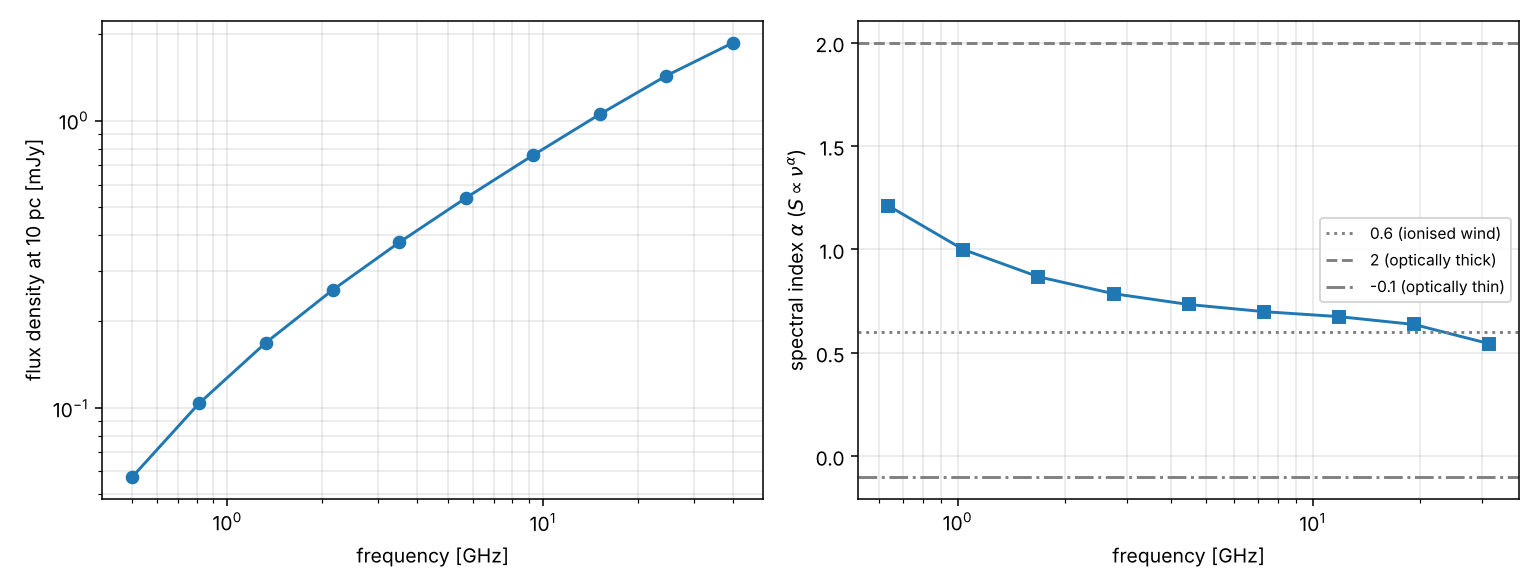
\includegraphics[width=0.9\textwidth]{fig/stellar_wind_spectrum.png}
\caption{Spectrum of the test wind ($64\,R_\ast$ field of view, Dulk Gaunt factor).
The spectral index approaches the wind value $\approx0.6$ at high frequency and is
larger at low frequency, where the $\tau=1$ surface fills the field of view.}\label{fig:windspec}
\end{figure}

%======================================================================
\chapter{One-dimensional (spherically symmetric) models}\label{chap:sym}
%======================================================================

A 1D model gives $n_e(r)$ and $T_e(r)$ only. Assuming spherical symmetry it produces a
radio image, but a circularly symmetric one: all its information is in the brightness
temperature as a function of the distance $p$ from the disk centre, and in the total
flux. Such images are useful as a \emph{diagnostic}:
\begin{itemize}[itemsep=1pt]
\item testing 1D coronal-heating and solar-wind models against radio data (the radio
  brightness depends on $n_e^2$ and $T_e$);
\item the quiet-Sun baseline: flux-density spectrum, apparent radius at each frequency, and
  azimuthally averaged brightness profiles from LOFAR, MWA, NoRH and other instruments;
\item stellar winds and coronae, which are observed unresolved (flux spectrum, spectral
  index, mass-loss rate);
\item fast parameter studies, and isolating the effect of refraction on the apparent size
  of the Sun.
\end{itemize}
They cannot reproduce maps of the real Sun (active regions, streamers, coronal holes).
1D support is provided for the mechanisms of the refractive ray tracer
(\code{bremsstrahlung}, \code{simplistic}, or your own emission function), with refraction
on or off. Gyroresonance and gyrosynchrotron are not offered for 1D models: a spherically
symmetric field is a magnetic monopole, and flare electrons are not spherically
symmetric.

\section{Loading a 1D model}
\begin{lstlisting}[style=pyex]
# from arrays: radii [R_sun], n_e [m^-3], T_e [K]
grid = rs.grid_from_profile(r, ne, te, r_body=1.0)
# from a text table (one radius per line); here r in cm, rho in g/cm^3, T in K
grid = rs.read_profile("model.txt", r_col=0, density_col=1, te_col=2,
                       r_unit=1 / 6.96e10, density="rho", density_unit="g/cm^3", mu_e=1.17)
# 1D spherical PLUTO output: read as a symmetric model automatically
grid = rs.load_pluto("out1d/")
# a star: coordinates in stellar radii
grid = rs.grid_from_profile(r, ne, te, length_unit=0.5 * rs.R_SUN)
\end{lstlisting}
The grid is an axisymmetric \code{SphericalGrid} with one colatitude cell spanning
$0\ldots\pi$, so it can be saved (\code{to\_npz}) and used with every function of
radiosynth, including the full 2D \code{make\_radio\_image}.

\section{Images, profiles and spectra}
\code{make\_symmetric\_image} traces only one row of rays, at distances
$p=0,\Delta p,\ldots,p_\text{max}$ from the centre, and rotates the result into a 2D
image. It is exact for a symmetric model (also with refraction and an observer at a finite
distance) and much faster than the full image:
\begin{lstlisting}[style=pyex]
img = rs.make_symmetric_image(grid, "80MHz, 150MHz, 300MHz, 1GHz, 17GHz", transfer="full",
                              x_size=6, nx=200, ny=200)           # no_refraction=True also works
img.profile["p"], img.profile["tb"], img.profile["flux"]          # radial profile, total flux
rs.plot_profile(img, path="profiles.png")
img.plot("tb")                                                    # the rotated image
\end{lstlisting}
\code{n\_p} (default 1000) is the number of rays: the brightness changes abruptly at the
limb, which needs fine sampling. \code{profile["flux"]} integrates
$S=2\pi D^{-2}\!\int_0^{p_\text{max}}I(p)\,p\,dp$ over the whole circle $p\le p_\text{max}$
(default $p_\text{max}$ = half the image diagonal), whereas \code{img.flux\_density} covers
the square field of view. All other keywords go to \code{make\_radio\_image}
(\code{transfer}, \code{gaunt}, \code{no\_refraction}, \code{distance\_pc}, \ldots).
For the five frequencies above the calculation takes about 15\,s, against about 10\,s
\emph{per frequency} for a $128\times128$ full image.

Command line:
\begin{lstlisting}
python -m radiosynth model.txt --profile --profile-cols 0 1 2 --profile-density rho \
       --profile-density-unit g/cm^3 --profile-r-unit 1.4368e-11 --symmetric \
       --freq "80MHz, 300MHz, 1GHz" --size 6 6 --transfer full --out quiet
python -m radiosynth out1d/ --symmetric --freq "150MHz" --out pluto1d
\end{lstlisting}
\code{--symmetric} writes the profile (\code{PREFIX\_profile.txt} and \code{.png}) and prints
the flux; the image files are written as usual.

\begin{figure}[h]\centering
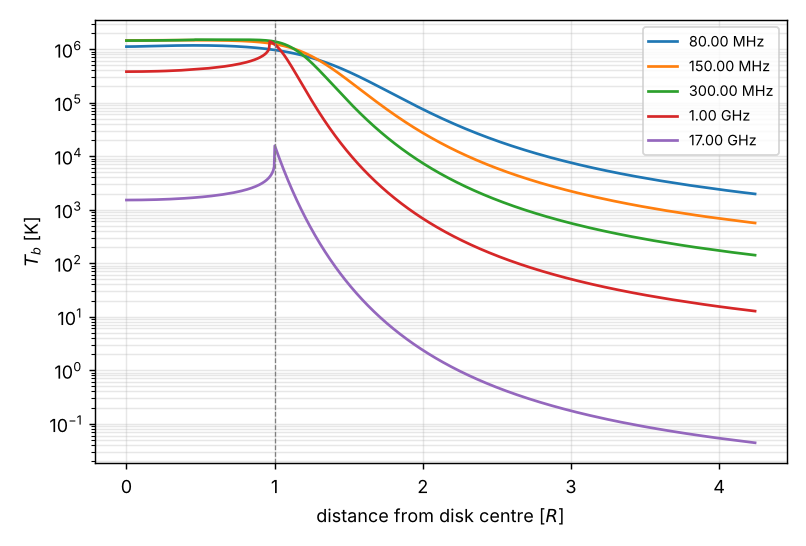
\includegraphics[width=0.49\textwidth]{fig/sym_profiles.png}\hfill
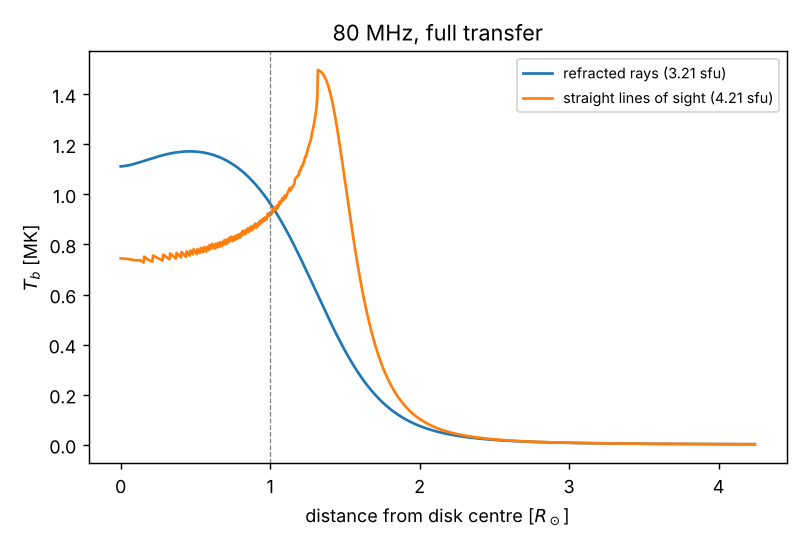
\includegraphics[width=0.49\textwidth]{fig/sym_refraction.png}
\caption{1D Newkirk corona (1.5\,MK). Left: $T_b(p)$ from 80\,MHz to 17\,GHz. Right:
80\,MHz with refracted rays and with straight lines of sight; refraction removes the bright
ring at the critical layer and reduces the flux by a quarter.}\label{fig:symprof}
\end{figure}

\begin{figure}[h]\centering
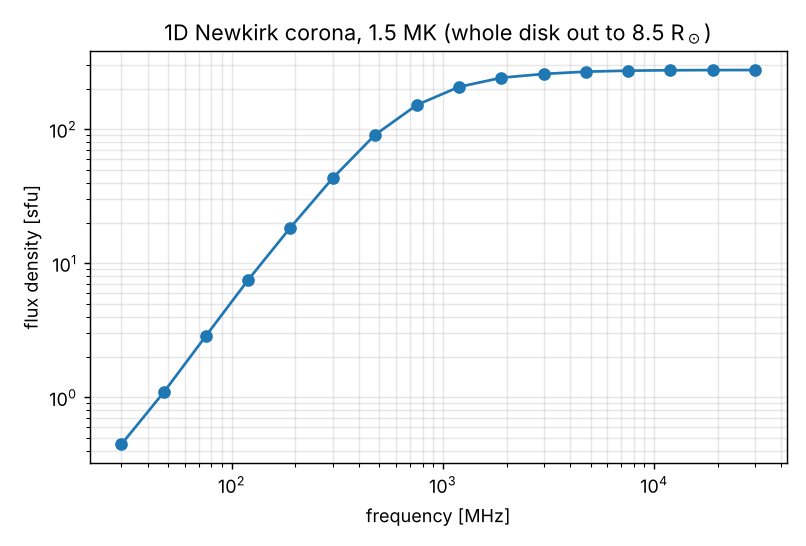
\includegraphics[width=0.55\textwidth]{fig/sym_spectrum.png}
\caption{Flux-density spectrum of the 1D corona, 30\,MHz--30\,GHz, from 16 symmetric
calculations.}\label{fig:symspec}
\end{figure}

\section{Accuracy}
The symmetric image agrees with the full 2D image of the same grid to $2\times10^{-4}$ in
flux and $3\times10^{-4}$ in $T_b$ along a row, and with a 3D Cartesian grid of the same
analytic corona to 0.1--2\%; for an optically thick stellar wind the profile flux agrees
with the exact integral to $2\times10^{-4}$ (Chapter~\ref{chap:validation}).

%======================================================================
\chapter{Gyroresonance emission and circular polarisation}\label{chap:gr}
%======================================================================

Above active regions the coronal magnetic field reaches hundreds to thousands of gauss.
Thermal electrons gyrating in such a field absorb and emit at the harmonics $s\nu_B$ of
the gyrofrequency $\nu_B=2.80\,\text{MHz}\times B[\text{G}]$. At a given frequency the
opacity is concentrated in thin \emph{harmonic layers}, the surfaces of constant field
strength
\begin{equation}
  |B| = \frac{\nu}{s\cdot2.80\,\text{MHz}}\qquad (s=1,2,3,\ldots),
\end{equation}
for example $|B|=595$\,G ($s=3$) and 893\,G ($s=2$) at 5\,GHz, and 2024\,G ($s=3$) at
17\,GHz. The $s=2$ and $s=3$ layers are usually optically thick in the extraordinary
(x) mode, so the radio image shows these iso-gauss surfaces at the local coronal
temperature: $T_b\approx T_e$ (1--3\,MK) wherever $|B|$ exceeds $\nu/(3\times2.8\,\text{MHz})$.
This makes gyroresonance images a direct test of the magnetic field \emph{and} the
temperature of an MHD model above active regions, at frequencies observed by the Nobeyama
Radioheliograph (17\,GHz), VLA, EOVSA (1--18\,GHz), RATAN-600, SSRT and the
Siberian/Chinese radioheliographs. Because the x- and o-modes have different opacities,
the emission is circularly polarised; Stokes $V$ maps the sign of the line-of-sight
field.

The \code{gyroresonance} folder computes these images from the model's $n_e$, $T_e$ and
$\vect B$, together with the free--free emission and absorption of the same plasma
(magnetised, i.e.\ different for the two modes). The physics is in
Chapter~\ref{chap:grtheory}.

\section{Step 1 --- Load the model with its magnetic field}

The magnetic field is optional in the grids; it is read only when asked for.

\paragraph{BATS-R-US.} Tecplot and IDL files contain \code{Bx By Bz}:
\begin{lstlisting}[style=pyex]
g = rs.load_mhd("3d__mhd_4_n00005000.dat", with_b=True)              # Tecplot: unit from "[Gauss]"
g = rs.load_mhd("box_ar.out", with_b=True, b_unit="nT")              # IDL file in nT
g = rs.load_mhd("box_ar.out", with_b=True, b_unit=2.2e2)             # normalised: gauss per unit
\end{lstlisting}
The unit is taken from the variable name (\code{[Gauss]}, \code{[G]}, \code{[nT]},
\code{[T]}). If the file does not give it, gauss is assumed with a warning; then pass
\code{b\_unit}. Scattered/AMR points are resampled together with $n_e$ and $T_e$.

\paragraph{PLUTO.} The cell-centred \code{bx1}, \code{bx2}, \code{bx3} are converted
from code units to gauss,
\begin{equation}
  B[\text{G}] = b\,\sqrt{4\pi\,\text{UNIT\_DENSITY}}\;\text{UNIT\_VELOCITY}\qquad(\text{cgs}),
\end{equation}
with the units from \code{definitions.h} as for the density (Chapter~\ref{chap:plutoobs}):
\begin{lstlisting}[style=pyex]
g = rs.load_pluto("out/", with_b=True)           # or rs.load_mhd("out/", with_b=True)
\end{lstlisting}
In spherical runs the components are $(B_r,B_\theta,B_\phi)$ and are rotated to
Cartesian at every sample point; 2.5D axisymmetric runs (with $B_\phi$) work as well.
Legacy VTK files written with \code{VTK\_VECTOR\_DUMP} contain Cartesian vectors, which
are recognised.

\paragraph{NumPy arrays.}
\begin{lstlisting}[style=pyex]
g = rs.MHDGrid(x, y, z, ne, te)           # coordinates in R_sun, ne [m^-3], te [K]
g.add_field(bx, by, bz)                   # [G], same shape as ne
s = rs.SphericalGrid(r, th, ph, ne, te)
s.add_field(br, bth, bph, components="spherical")
g.to_npz("ar.npz"); g = rs.load_mhd("ar.npz")     # B is saved and reloaded
\end{lstlisting}

\begin{warn}[Resolution]
The optical depth of a layer is proportional to the magnetic scale length
$L_B=|B|/|dB/d\ell|$, which the code takes from the field at the sample points. Use a grid
that resolves the active region (cells of a few Mm, i.e.\ $\lesssim0.005\,\rsun$) and
restrict the box to the region of interest: a global model with 0.05\,\rsun{} cells gives
only a rough picture of an active region.
\end{warn}

\section{Step 2 --- Compute the image}

\begin{lstlisting}[style=pyex]
img = rs.make_gr_image(g, "3GHz, 5GHz, 10GHz, 17GHz",
                       observer=(-215, 0, 0),          # or rs.figures.observer_for_date(...)
                       x_size=0.4, y_size=0.4, nx=200, ny=200)   # field of view in R_sun
print(img.summary())
img.plot("tb"); img.plot("pol"); img.plot("harmonic")
\end{lstlisting}

\begin{longtable}{@{}p{3.3cm}p{11.9cm}@{}}
\toprule
Parameter & Meaning \\
\midrule\endhead
\code{observer}, \code{x\_size}, \code{y\_size}, \code{nx}, \code{ny}, \code{up}, \code{distance\_pc}, \code{r\_integration} &
  As in \code{make\_radio\_image}: image plane through the centre, pixel layout, observer at a
  distance or (with \code{distance\_pc}) a star with parallel rays. The default field of
  view is $2\times2\,\rsun$; active regions need much less. \\
\code{mechanisms} & \code{"gr+ff"} (default): layers and magnetised free--free in one
  transfer; \code{"gr"}: layers only; \code{"ff"}: magnetised free--free only. \\
\code{gaunt} & Free--free Gaunt factor: \code{"dulk"} (default here) or a number. \\
\code{s\_max} & Highest harmonic considered (default 10; layers above $s\approx5$ are
  optically thin for coronal temperatures). \\
\code{coupling} & \code{"weak"} (default): the sense of circular polarisation is conserved
  where $\vect B\cdot\vect k$ changes sign along the ray (usual at microwaves);
  \code{"strong"}: the mode is conserved and the sense of polarisation flips there. \\
\code{ds} & Step along the rays [\rsun]; default half the smallest cell. The layers are
  located exactly between the sample points, so \code{ds} only needs to resolve the
  variation of the fields. \\
\code{t\_body} & Brightness temperature of the body (e.g.\ $10^4$\,K for the
  chromosphere) behind rays that reach $r_\text{body}$; default none, as in the
  refractive tracer. \\
\code{max\_points} & Memory control: number of samples processed at once (default $4\times10^5$). \\
\bottomrule
\end{longtable}

A $200\times200$ image of an active region on a $120^3$ grid takes about 3\,s per
frequency on one core.

\section{Step 3 --- The result: \code{GRImage}}\label{sec:grout}

\code{GRImage} is a \code{RadioImage}, so \code{brightness\_temperature},
\code{flux\_density}, \code{flux\_density\_sfu}, \code{save\_fits}, \code{save\_tecplot} and
all figure and comparison functions work. In addition:

\begin{center}\small
\begin{tabularx}{\textwidth}{@{}l X@{}}
\toprule
Attribute & Content \\
\midrule
\code{intensity} & Stokes $I=I_1+I_2$ [W m$^{-2}$ Hz$^{-1}$ sr$^{-1}$]. \\
\code{stokes\_v}, \code{tb\_v} & Stokes $V$; $V>0$ is right-hand circular polarisation (IAU/IEEE). \\
\code{polarization} & $V/I$. \\
\code{pol1}, \code{pol2}, \code{pol\_names} & The two polarisations: $R$, $L$ (weak coupling) or $x$, $o$ (strong). \\
\code{tb\_pol} & Their brightness temperatures $T_p=I_pc^2/(k_B\nu^2)$; each equals $T_e$ where thick. \\
\code{tau}, \code{tau2} & Optical depth along the ray in polarisation 1 and 2. \\
\code{dominant\_s} & Harmonic that produces most of the intensity (0 = free--free, $-1$ = no emission). \\
\code{radius} & Intensity-weighted radius of the emitting layer [\rsun]; height $=$ radius $-1$. \\
\code{gr\_fraction} & Fraction of $I$ from gyroresonance layers. \\
\code{x\_flag} & True where an important layer has $(\nu_p/\nu)^2>0.25$, where the straight-ray, $n=1$ approximation is rough. \\
\code{flux\_density\_v} & Flux density of Stokes $V$. \\
\bottomrule
\end{tabularx}
\end{center}

\code{plot(quantity)} accepts \code{"tb"}, \code{"intensity"}, \code{"v"},
\code{"pol"}, \code{"harmonic"}, \code{"radius"} and \code{"gr\_fraction"};
\code{save\_fits(path, quantity)} also writes \code{"v"}, \code{"tb\_v"} and
\code{"pol"}; \code{save\_npz} saves everything.

\section{Example: a bipolar active region}

\code{examples/active\_region.py} builds an analytic active region: a horizontal dipole
35\,Mm below disk centre (2500\,G above it, a positive spot on the left of the image and a
negative one on the right), in a hydrostatic corona with $n_e=2\times10^{9}$\,cm$^{-3}$ at
the base, a 35\,Mm scale height and $T_e=2.5$\,MK. \code{examples/gyroresonance\_example.py}
makes the figures below.

\begin{figure}[h]\centering
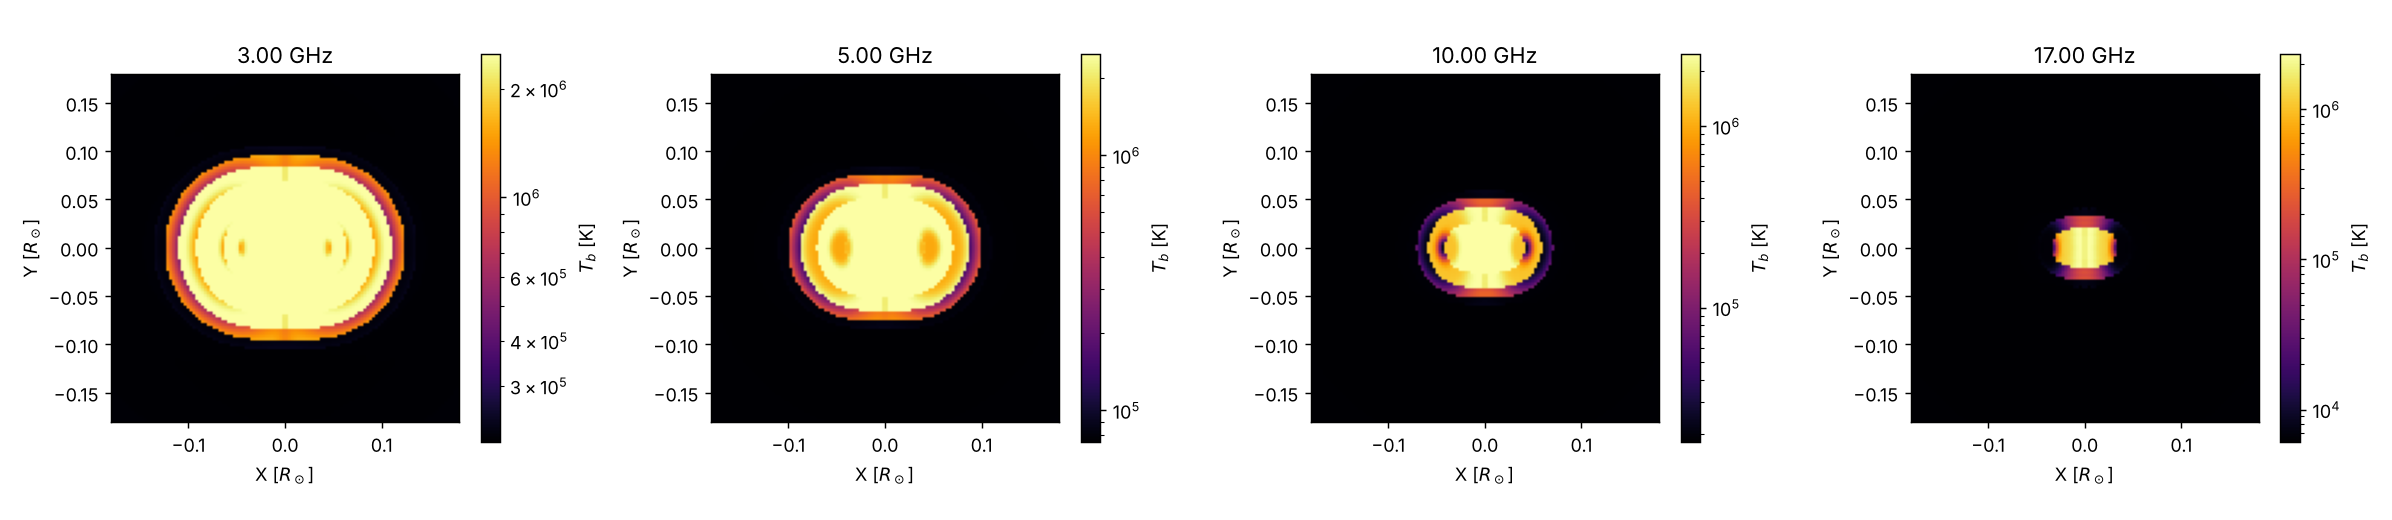
\includegraphics[width=\textwidth]{fig/gr_tb.png}\\[-1mm]
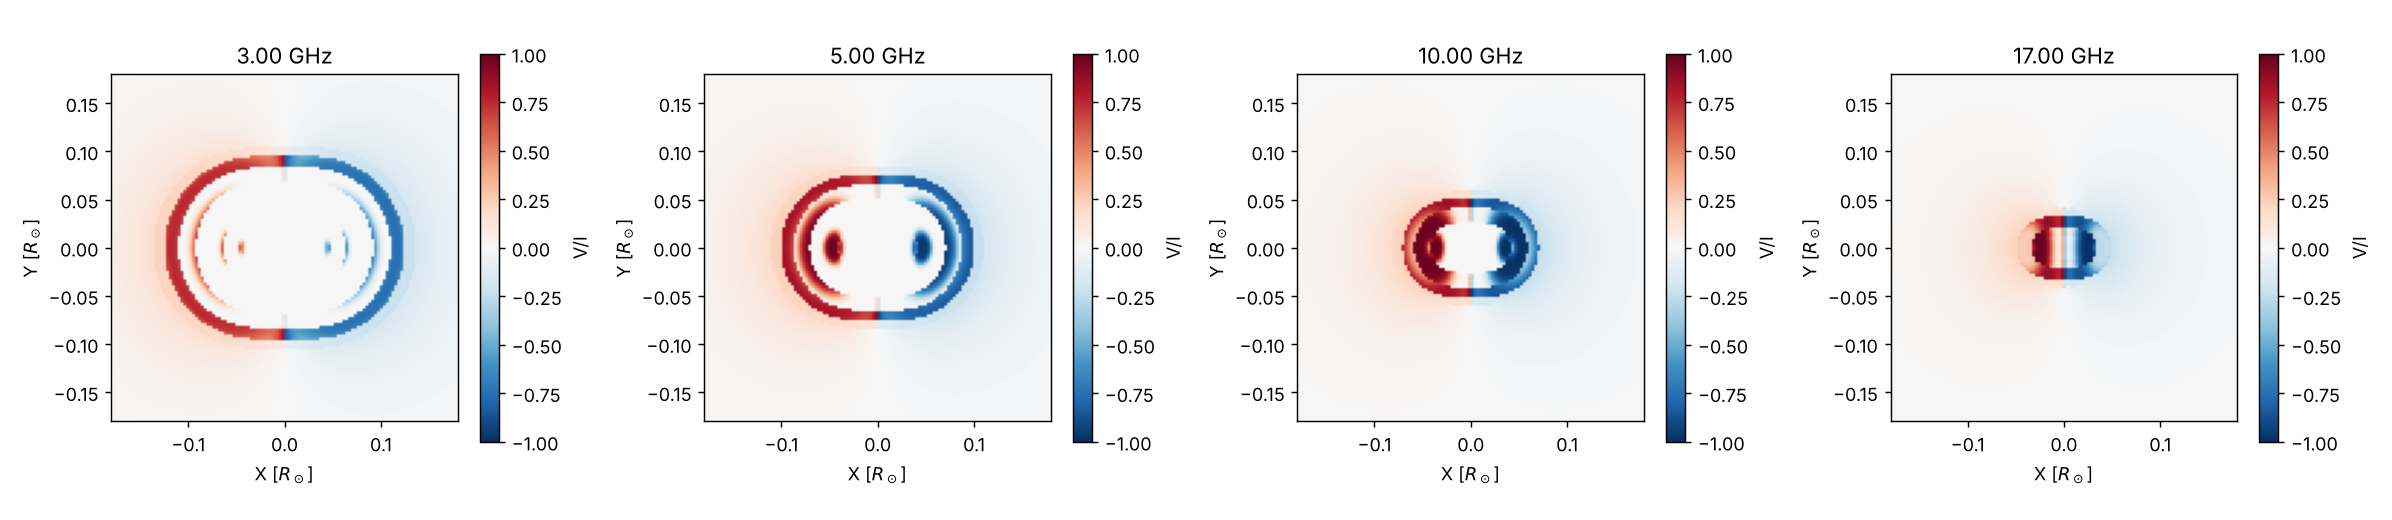
\includegraphics[width=\textwidth]{fig/gr_pol.png}\\[-1mm]
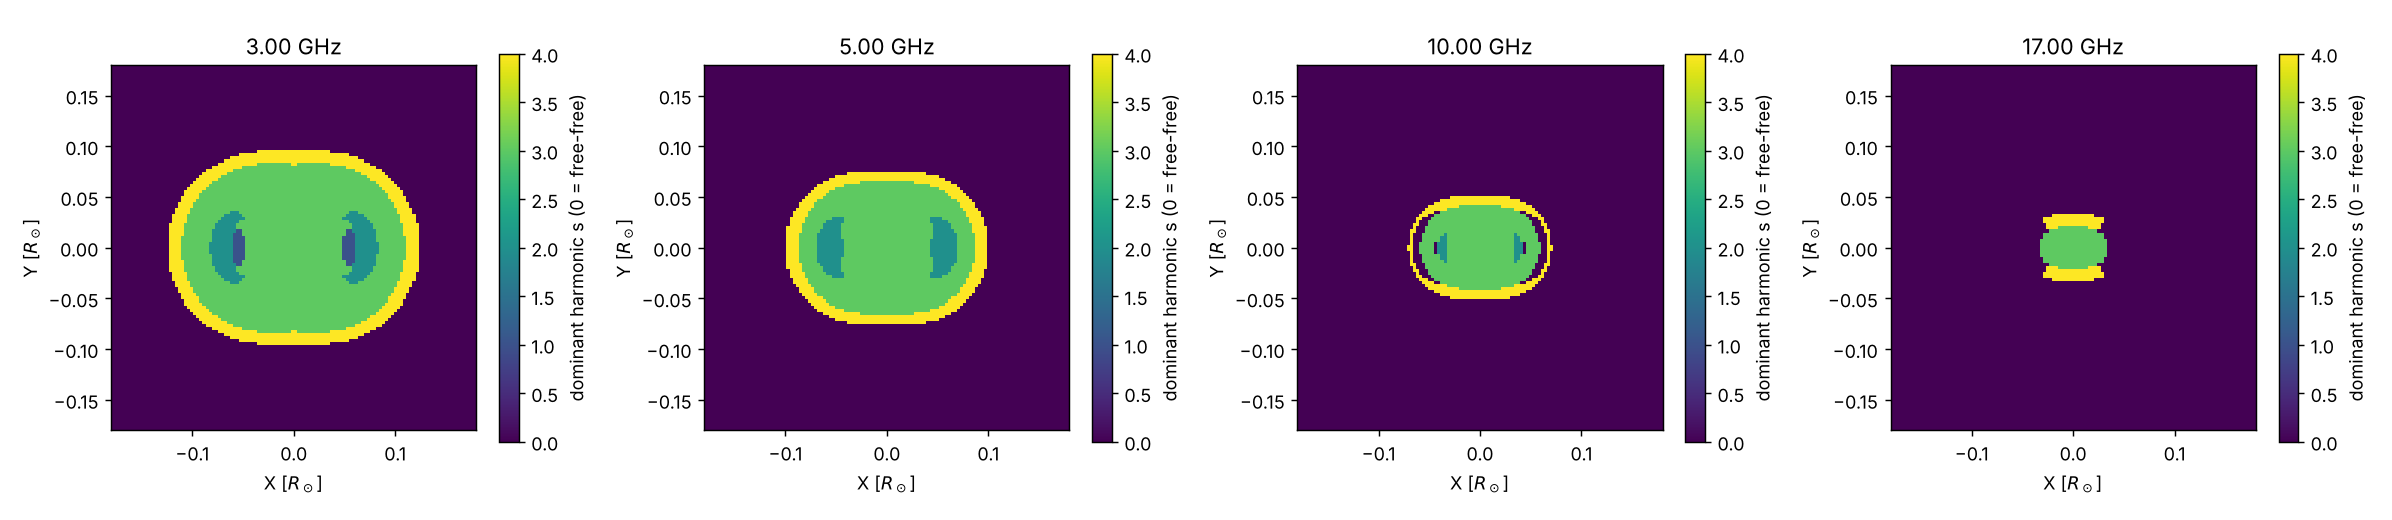
\includegraphics[width=\textwidth]{fig/gr_harmonic.png}
\caption{Gyroresonance + free--free images of the bipolar active region at 3, 5, 10 and
17\,GHz. Top: $T_b$; middle: degree of circular polarisation $V/I$; bottom: dominant
harmonic (0 = free--free).}\label{fig:grar}
\end{figure}

How to read Figure~\ref{fig:grar}:
\begin{itemize}[itemsep=2pt]
\item The bright region is bounded by the outermost optically thick layer, here
  $s=4$ at 3\,GHz and $s=3$--4 at higher frequencies; inside it $T_b=T_e=2.5$\,MK. It
  shrinks with frequency because a higher frequency needs a stronger field.
\item Straight above each spot the field is nearly along the line of sight. The
  opacity of the layers with $s\ge2$ is proportional to $\sin^{2(s-1)}\theta$, so the
  $s=3$ layer becomes thin there. The emission then comes from the deeper $s=2$ layer,
  which is itself only partly thick at small $\theta$, so $T_b$ drops below $T_e$: a
  central depression over each spot, as predicted by gyroresonance theory and seen in
  some observed sunspot sources.
\item $V/I$ is large ($\approx\pm1$) in a ring at the edge of the source: there the x-mode
  is still thick but the o-mode is not. Where both are thick (the core) $V/I\to0$. The
  sign follows the line-of-sight field: positive (RCP) over the positive spot. In
  observations this ring pattern and the sign reversal across the neutral line are
  diagnostics of the field geometry.
\item Free--free emission (harmonic 0) gives the faint $\sim10^5$\,K halo.
\end{itemize}

\paragraph{Which mechanism dominates?}\label{sec:grmech}
Figure~\ref{fig:grmech} compares the three settings of \code{mechanisms}. The combined
image is close to the gyroresonance-only one where the layers are thick, because the
free--free emission of the plasma behind (below) a thick layer is hidden. The
free--free-only image shows what the same plasma would look like without a field.

\begin{figure}[h]\centering
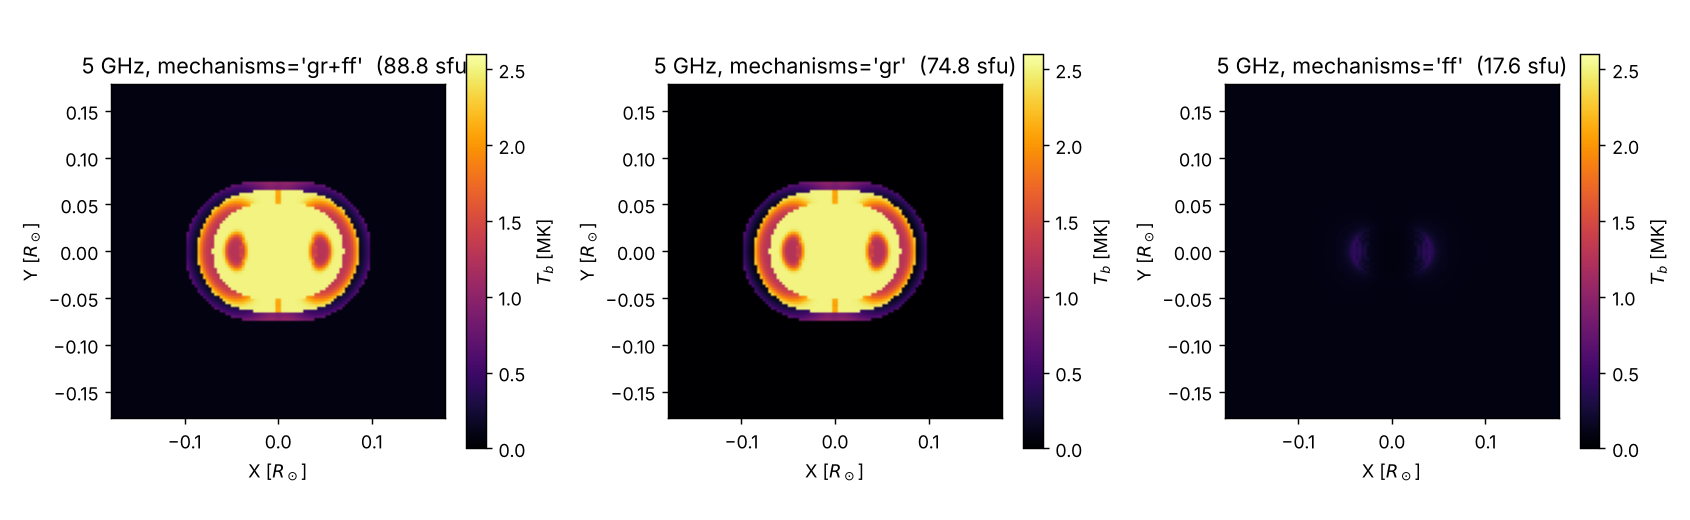
\includegraphics[width=\textwidth]{fig/gr_mech.png}
\caption{5\,GHz images computed with \code{mechanisms="gr+ff"}, \code{"gr"} and
\code{"ff"}.}\label{fig:grmech}
\end{figure}

\begin{figure}[h]\centering
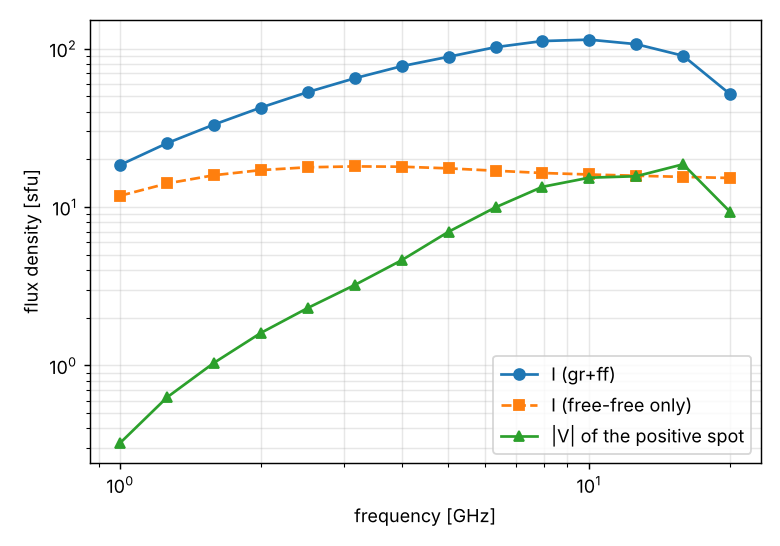
\includegraphics[width=0.62\textwidth]{fig/gr_spectrum.png}
\caption{Flux-density spectrum of the active region: total (gyroresonance + free--free),
free--free alone, and $|V|$ of the positive spot. The total $V$ of a balanced bipolar
region is close to zero.}\label{fig:grspec}
\end{figure}

The spectrum (Figure~\ref{fig:grspec}) rises with frequency while the area inside the
thick layers stays large, peaks near 10\,GHz and falls steeply once the $s=3$ layer
shrinks into the spot umbrae; the frequency of this turnover measures the maximum
coronal field strength.

\section{Comparison with observations}

\begin{itemize}[itemsep=2pt]
\item Orient the model as for free--free maps (Section~\ref{sec:orient}): the image
  plane, observer and helioprojective axes are the same, so \code{observer\_for\_date},
  \code{fit\_longitude\_offset} and \code{compare\_with\_observation} work unchanged.
\item Convolve the synthetic map with the instrument beam before comparing peak $T_b$
  (\code{gaussian\_filter} from \code{scipy.ndimage}, with the beam width in pixels): gyroresonance
  sources are compact and beams of 5--20$''$ lower their peak.
\item Compare $T_b$ \emph{and} $V$: $I$ tests the field strength and temperature, $V$
  the line-of-sight field direction and the mode structure. Nobeyama (17\,GHz) and
  RATAN-600 give $V$; EOVSA gives spectra 1--18\,GHz per pixel, to be compared with
  \code{img.brightness\_temperature[:, j, i]} over many frequencies.
\item Most MHD models have no chromosphere; set \code{t\_body=1e4} to give the disk its
  chromospheric $T_b$ where no layer is in front.
\end{itemize}

\paragraph{Stars.} With \code{distance\_pc} the same calculation gives the flux density
and circular polarisation of stellar active regions (e.g.\ M dwarfs, RS CVn binaries):
\code{img.flux\_density\_mjy}, \code{img.flux\_density\_v}.

\section{Approximations and limitations}\label{sec:grlimits}
\begin{itemize}[itemsep=2pt]
\item \textbf{Thermal, single-temperature Maxwellian} at each point. Non-thermal
  gyrosynchrotron emission from flares and multithermal (DEM) effects are not included.
\item \textbf{Lowest order in $\beta_T$} (small Larmor radius) and \textbf{refractive
  index 1} in the layer opacity. The o-mode opacity at nearly perpendicular propagation is
  of higher order in $\beta_T$ and is underestimated; this affects $V$ in narrow strips
  where $\vect B\perp$ the line of sight.
\item \textbf{Straight rays}. Valid where the layers form at $\nu\gg\nu_p$; pixels where a
  layer forms at $(\nu_p/\nu)^2>0.25$ are flagged in \code{x\_flag}.
\item \textbf{Mode coupling} is treated in the two limits (weak or strong) only, not by
  solving the coupling equations in quasi-transverse regions.
\item \textbf{Magnetised free--free} uses $\kappa_\sigma=\kappa/(1\pm Y|\cos\theta|)^2$,
  valid for $Y<1$ away from quasi-transverse propagation; where gyroresonance dominates
  this does not matter.
\item The layers must be resolved by the model ($L_B$ from neighbouring sample points).
\end{itemize}

%======================================================================
\chapter{Gyrosynchrotron emission of fast electrons}\label{chap:gs}
%======================================================================

During flares, in CME cores and in the coronae of active stars, mildly relativistic
electrons (tens of keV to MeV) gyrating in the magnetic field produce
\emph{gyrosynchrotron} emission: a broad continuum, usually peaking at 5--20\,GHz, with
brightness temperatures far above the plasma temperature. Computing it accurately
requires sums over many harmonics and integrals over the electron distribution. This is
what the public \emph{fast gyrosynchrotron codes} of Fleishman \& Kuznetsov (2010) and
Kuznetsov \& Fleishman (2021) do; they are also the engine of GX Simulator.

The \code{gyrosynchrotron} folder does \emph{not} re-implement them. It uses them as a
compiled library:
\begin{itemize}[itemsep=1pt]
\item radiosynth provides the lines of sight and the plasma along them: the image
  geometry and observers (as for every other mechanism), straight rays cut into voxels,
  and in every voxel its length, $n_e$, $T_e$, $|\vect B|$, the angle between $\vect B$
  and the line of sight, and the parameters of the fast electrons from your prescription;
\item the library computes the emission, absorption and radiative transfer along each
  line of sight (gyrosynchrotron of the fast electrons, free--free of the thermal plasma,
  both magneto-ionic modes and their coupling), for many lines of sight in parallel;
\item radiosynth converts the result to an image with Stokes $I$ and $V$ and all the usual
  outputs.
\end{itemize}

\section{Installing the fast GS codes}
The codes are distributed under the GNU GPL v3 at
\url{https://github.com/kuznetsov-radio/gyrosynchrotron} and are \emph{not} included in
radiosynth. Build them once (needs \code{git}, \code{make}, \code{g++} with OpenMP; on
macOS \code{brew install libomp}):
\begin{lstlisting}
python -m radiosynth.gyrosynchrotron.library --build      # -> ~/.radiosynth/gyrosynchrotron
\end{lstlisting}
or from Python \code{rs.gyrosynchrotron.build\_library()}. If compilation is not possible
the prebuilt binary of the repository for your platform is used. The library is searched
for in the \code{library=} argument, in the environment variable
\code{RADIOSYNTH\_GSCODES} (file or folder), and in \code{\textasciitilde/.radiosynth/gyrosynchrotron/binaries/}.
The version (git commit) is printed with every image. Use \code{OMP\_NUM\_THREADS} to set
the number of threads.

\section{Describing the fast electrons}
An MHD model has no fast electrons, so they are prescribed with a
\code{FastElectrons} object. Each parameter is a number or a \emph{rule}: a function of the
quantities sampled at every voxel (\code{pos}, \code{r}, \code{ne} [m$^{-3}$],
\code{te}, \code{b}, \code{bmag} [G], and grid scalar fields such as the current density
\code{j}).

\begin{center}\small
\begin{tabularx}{\textwidth}{@{}l X@{}}
\toprule
Parameter & Meaning \\
\midrule
\code{nb} & Fast-electron density [cm$^{-3}$] (number or rule). Typical flare values $10^6$--$10^9$ above 10\,keV. \\
\code{energy} & \code{"plw"} power law (default), \code{"dpl"} double power law, \code{"kap"} kappa, \code{"tnt"} thermal + power-law tail, \code{"tpl"} isotropic thermal + power law, \code{"plp"}, \code{"plg"} power laws in momentum or Lorentz factor. \\
\code{delta} (\code{delta2}, \code{ebreak\_mev}) & Power-law index (high-energy index and break energy for \code{"dpl"}); typical 2.5--5. \\
\code{emin\_mev}, \code{emax\_mev} & Energy range (default 0.01--10 MeV). \\
\code{kappa}, \code{eps} & Parameters of the kappa and thermal/non-thermal distributions. \\
\code{pitch} & \code{"iso"} (default), \code{"gau"} or \code{"elc"} loss cone, \code{"gab"} or \code{"sga"} beam. \\
\code{alpha\_c}, \code{dmu}, \code{a4} & Loss-cone angle or beam direction [deg], width, super-gaussian exponent. \\
\code{nb\_min} & Below this $n_b$ the voxel gets no fast electrons (saves time; default 1\,cm$^{-3}$). \\
\bottomrule
\end{tabularx}
\end{center}

Rules for $n_b$ (\code{radiosynth.gyrosynchrotron}):
\begin{lstlisting}[style=pyex]
from radiosynth.gyrosynchrotron import (FastElectrons, uniform, fraction_of_thermal,
                                        power_of, in_sphere, in_box, product)
in_sphere((-1.04, 0, 0), 0.015, 1e7)          # gaussian blob, e.g. at a loop top
fraction_of_thermal(1e-3)                      # n_b = 1e-3 n_e
power_of("bmag", 1e7, 500.0, power=2)          # n_b = 1e7 (B/500 G)^2
rs.current_density(grid)                       # adds the scalar 'j' = |J| [A/m^2]
power_of("j", 1e7, ref=jmax, floor=0.2)        # at current concentrations
product(fraction_of_thermal(1e-3), in_box(lo, hi, 1.0))   # combinations
lambda f: 1e7 * (f["r"] < 1.05)                # any function of the sampled fields
\end{lstlisting}
A tabulated distribution (for example from test-particle or Fokker--Planck results) is
given with \code{FastElectrons.from\_array(E\_mev, mu, f, nb=rule)}: the shape $f(E,\mu)$ is
normalised to unit density and multiplied by the local $n_b$; it is passed to the codes as
their numerically defined distribution.

\begin{note}[Choosing the prescription]
The images depend strongly on these choices, so state them with the results. Constrain
them where possible: hard X-ray spectra give $\delta$, $E_\text{min}$ and the electron
flux (the microwave-emitting electrons are often harder, $\delta_\text{MW}\approx\delta_\text{HXR}-1$);
microwave spectra constrain $n_b$ and $\delta$; polarisation constrains the field and the
pitch-angle distribution. The code prints the largest ratio of the fast-electron to the
magnetic energy density; values above $\sim$0.1 indicate an unphysical prescription.
\end{note}

\section{Computing the image}
\begin{lstlisting}[style=pyex]
grid = rs.load_mhd("flare.dat", with_b=True)
el = rs.FastElectrons(nb=rs.gyrosynchrotron.in_sphere((-1.04, 0, 0), 0.015, 1e7),
                      delta=3.5, emin_mev=0.02, emax_mev=5.0)
img = rs.make_gs_image(grid, "3GHz, 5GHz, 10GHz, 17GHz", el,
                       x_size=0.36, y_size=0.36, nx=100, ny=100, diagnostics=True)
img.plot("tb"); img.plot("pol"); img.plot("gs_fraction")
\end{lstlisting}

\begin{longtable}{@{}p{3.3cm}p{11.9cm}@{}}
\toprule
Parameter & Meaning \\
\midrule\endhead
\code{observer}, \code{x\_size}, \ldots, \code{distance\_pc} & As for the other mechanisms. \\
\code{coupling} & Mode coupling in the library: \code{"exact"} (default), \code{"weak"}, \code{"strong"}. \\
\code{free\_free} & Include free--free emission and absorption of the thermal plasma (default). \\
\code{gyrosynchrotron} & \code{False}: no fast electrons (the library's free--free only). \\
\code{abundance} & Free--free opacity: \code{"coronal"} (default), \code{"photospheric"}, \code{"dulk"}. \\
\code{ds} & Voxel length [\rsun]; default half the smallest cell. \\
\code{t\_body} & Brightness temperature of the body behind the plasma. \\
\code{diagnostics} & Also compute free--free alone: \code{gs\_fraction} $=1-I_\text{ff}/I$. \\
\code{fc}, \code{fwh}, \code{nnodes}, \code{q\_optimization} & Accuracy and speed controls of the hybrid GS code (library defaults). \\
\code{library} & Path of the compiled codes. \\
\code{max\_voxels} & Voxels per library call (memory). \\
\bottomrule
\end{longtable}

The result is a \code{GSImage}: Stokes $I$ (\code{intensity}), \code{stokes\_v} ($V>0$
right-hand, as everywhere in radiosynth), \code{pol1}/\code{pol2} ($R$/$L$),
\code{polarization}, \code{gs\_fraction}, and all \code{RadioImage} methods. The library
does not return optical depths (\code{tau} is NaN).

Cost: only voxels with fast electrons are expensive. The example below
($60\times60$ pixels, 4 frequencies, blob of $\sim$10\,Mm) takes about 40\,s on 2 cores.

\section{Example: fast electrons at the top of the active-region arcade}

\code{examples/gyrosynchrotron\_example.py} places a gaussian blob of fast electrons
($n_b=10^7$\,cm$^{-3}$ above 20\,keV, $\delta=3.5$, isotropic) 35\,Mm above the centre of
the bipolar region of Chapter~\ref{chap:gr}, where $|B|\approx430$\,G.

\begin{figure}[h]\centering
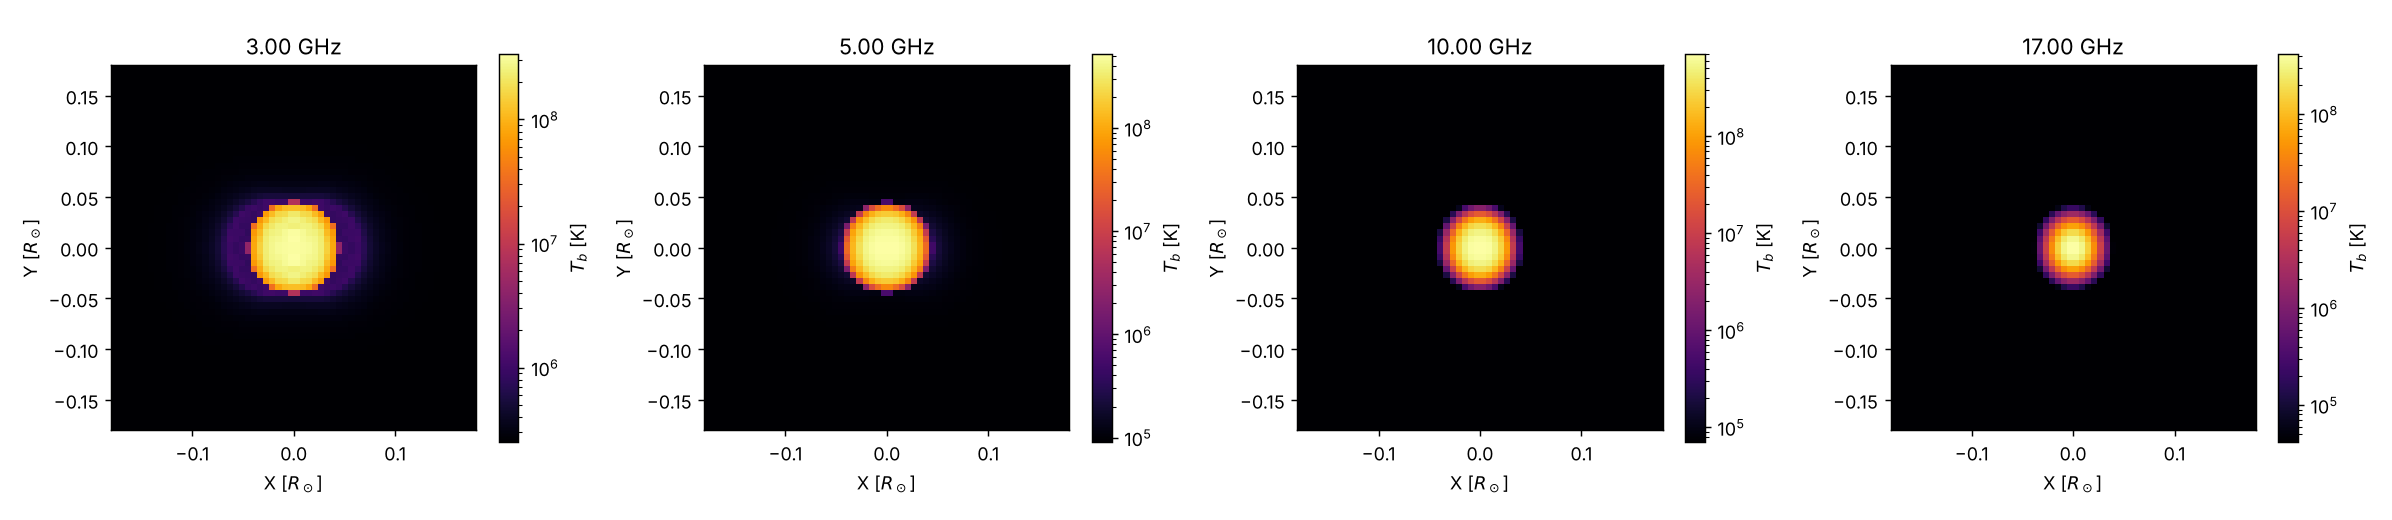
\includegraphics[width=\textwidth]{fig/gs_tb.png}\\[-1mm]
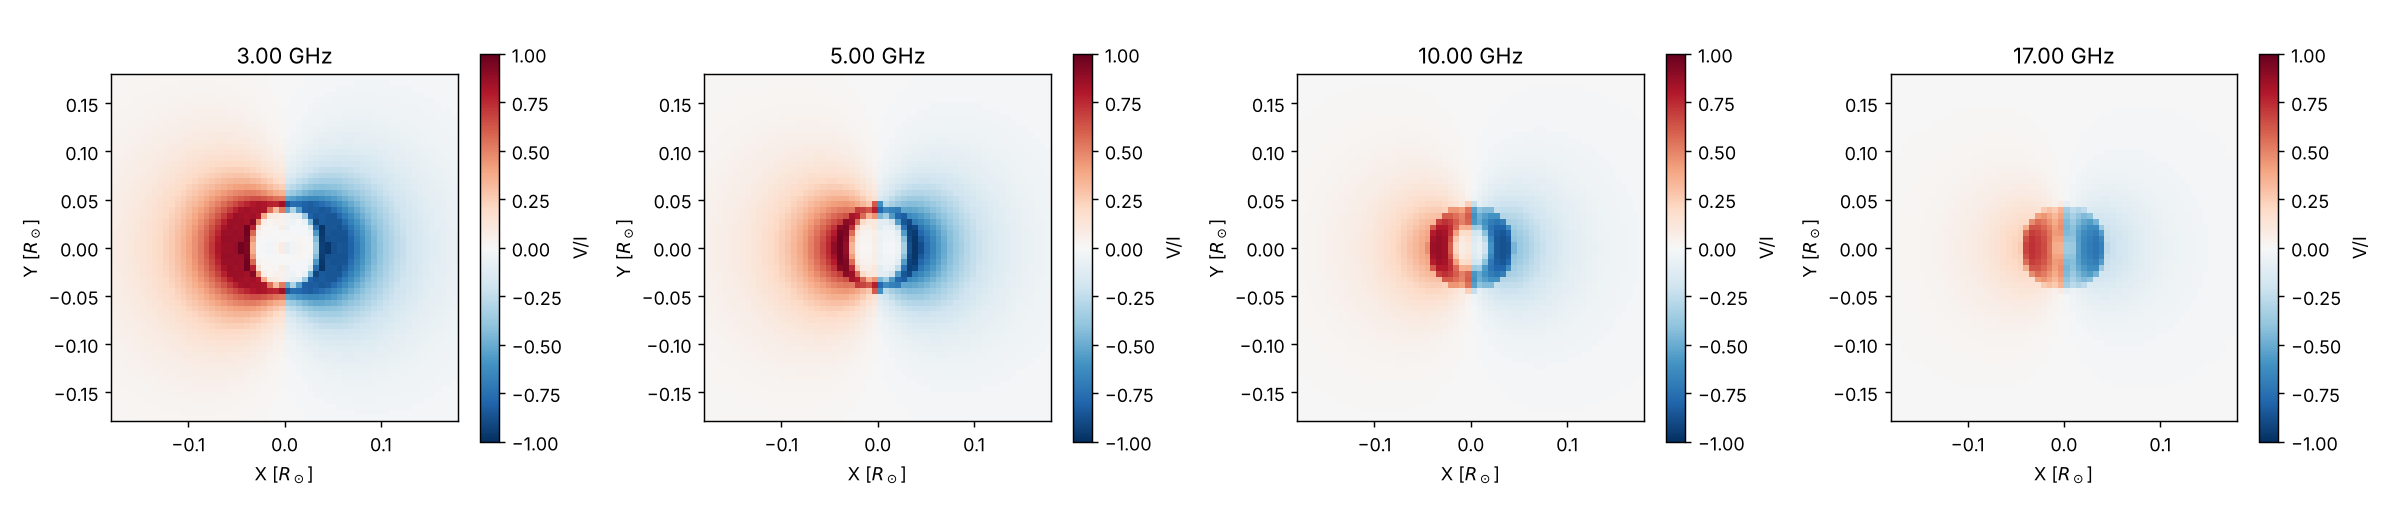
\includegraphics[width=\textwidth]{fig/gs_pol.png}\\[-1mm]
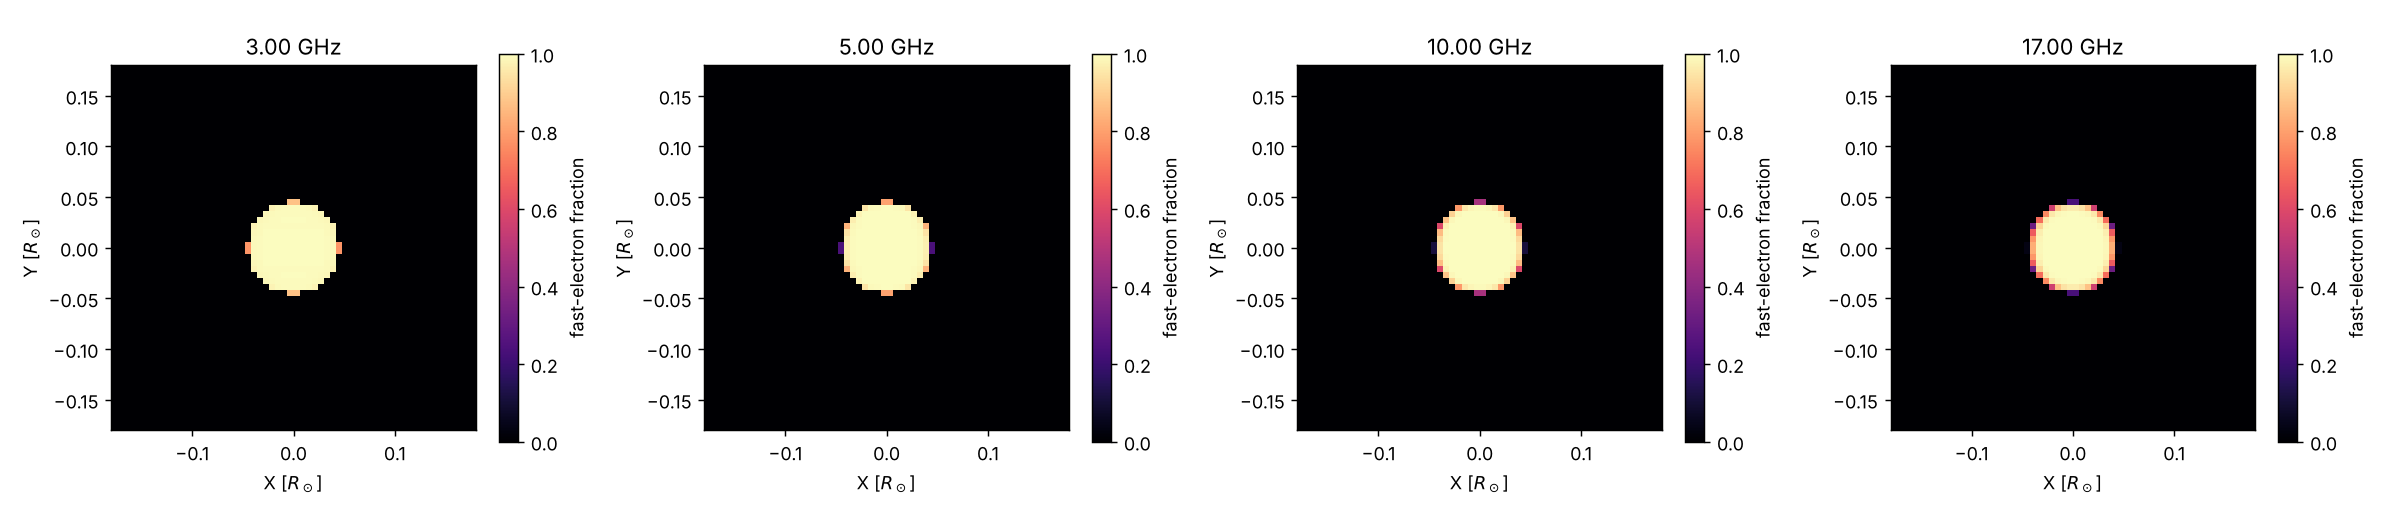
\includegraphics[width=\textwidth]{fig/gs_fraction.png}
\caption{Gyrosynchrotron + free--free images at 3, 5, 10 and 17\,GHz. Top: $T_b$;
middle: $V/I$; bottom: fraction of the intensity due to the fast electrons.}\label{fig:gsimg}
\end{figure}

The source is optically thick at low frequencies ($T_b\sim3\times10^8$\,K, set by the
effective temperature of the emitting electrons, and $V/I\approx0$ in its centre) and
thin above the spectral peak, where it shrinks to the strongest field and its edges are
polarised with the sign of the line-of-sight field. The free--free emission of the
surrounding thermal plasma is visible as the faint polarised halo.

\begin{figure}[h]\centering
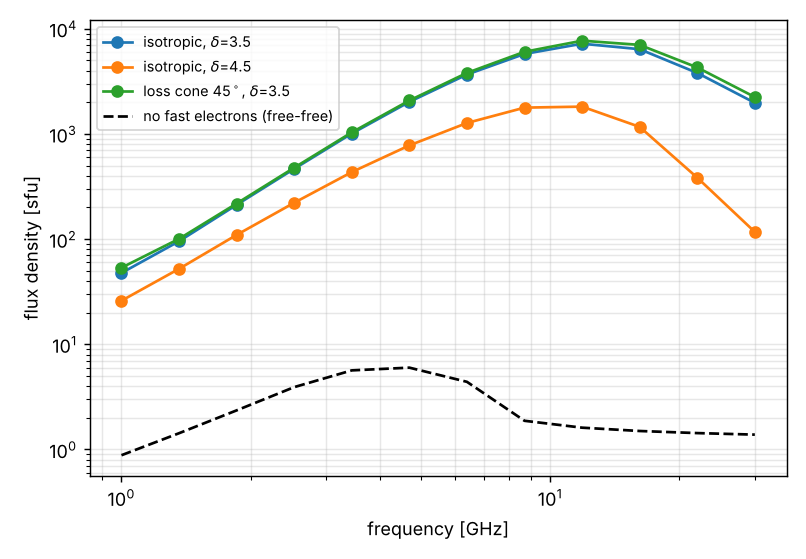
\includegraphics[width=0.6\textwidth]{fig/gs_spectrum.png}
\caption{Flux spectrum of the blob for three prescriptions, and of the same region
without fast electrons.}\label{fig:gsspec}
\end{figure}

Figure~\ref{fig:gsspec} shows the classic gyrosynchrotron spectrum: rising as an
optically thick source at low frequencies, peaking near 10\,GHz, and falling as a power
law above, the steeper the larger $\delta$. A loss cone barely changes the flux for this
viewing angle. Figure~\ref{fig:gstrap} uses a different prescription: a trapped population
$n_b=10^{-3}n_e$ in the core of the arcade.

\begin{figure}[h]\centering
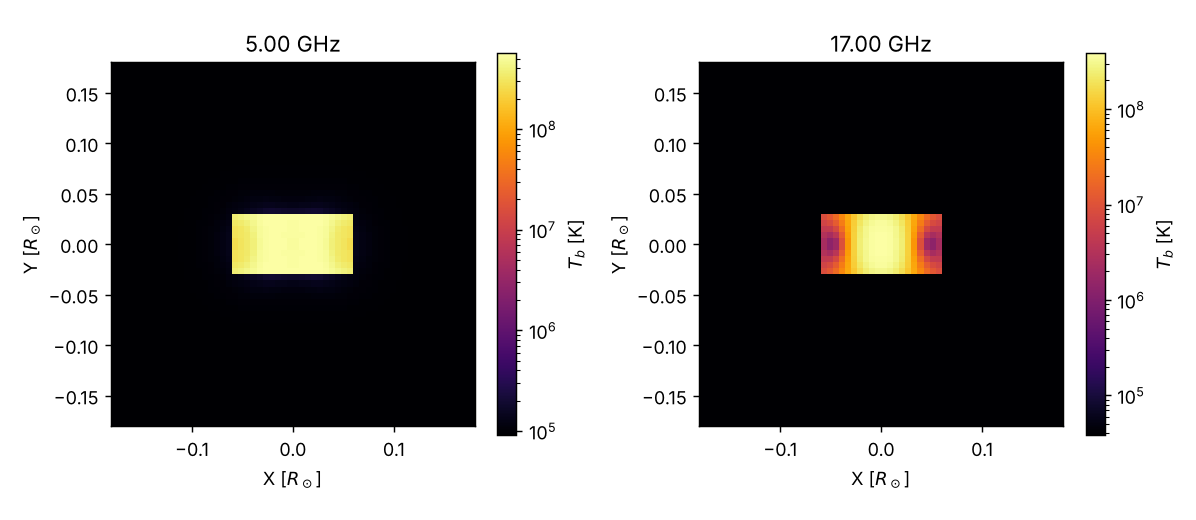
\includegraphics[width=0.62\textwidth]{fig/gs_trapped.png}
\caption{Fast electrons as a fixed fraction of the thermal density in a box around the
arcade core (gaussian loss cone, $\alpha_c=45^\circ$).}\label{fig:gstrap}
\end{figure}

\section{Relation to the other mechanisms; limitations}
\begin{itemize}[itemsep=2pt]
\item The thermal plasma contributes \textbf{free--free} emission in the library (with
  its own Coulomb logarithm and abundances: about 15--20\% above radiosynth's Dulk formula
  for the same plasma, Chapter~\ref{chap:validation}). \textbf{Thermal gyroresonance} is not
  included: the library treats each voxel as homogeneous, which does not resolve the thin
  harmonic layers. To have the layers and the fast electrons together, absorbing each
  other, use the \code{combined} folder (Chapter~\ref{chap:combined}).
\item The library's source function contains the refractive index, $S=n_\sigma^2B_\nu$, so
  an optically thick dense source has $T_b=n_\sigma^2T_e$; this matters only where
  $(\nu_p/\nu)^2$ is not small.
\item Straight rays, as for gyroresonance.
\item The fast electrons are prescribed, not computed (see the note on choosing the
  prescription); the energy check guards against unphysical choices only.
\end{itemize}

%======================================================================
\chapter{Combined images: free--free, gyroresonance and gyrosynchrotron}\label{chap:combined}
%======================================================================

In an active region during a flare all three processes radiate at the same
frequencies, and they \emph{absorb each other}: an optically thick gyroresonance layer
hides a gyrosynchrotron source behind it, fast electrons absorb the thermal emission
behind them, and dense plasma attenuates everything by free--free absorption. The
combined image is therefore not the sum of the three separate images. The
\code{combined} folder puts the three into \emph{one} polarised radiative transfer along
every line of sight.

\section{How it works}
\begin{itemize}[itemsep=2pt]
\item The lines of sight are straight and sampled exactly as for gyroresonance; the
  free--free (two modes) and the harmonic layers are computed by radiosynth as in
  Chapter~\ref{chap:gr}.
\item For every voxel that contains fast electrons, the fast GS codes are called with the
  voxel alone as the line of sight, twice: without incoming radiation (giving the emitted
  intensity $E$) and with a known incoming intensity $I_\text{in}$ (giving
  $I_\text{in}e^{-\tau}+E$). This gives the gyrosynchrotron optical depth $\tau$ and
  emission of the voxel in both circular polarisations; the codes' own free--free is
  switched off in these calls, so nothing is counted twice. All such voxels go to the
  library in one multi-threaded call.
\item In every step of the transfer the optical depths of the three processes add, and the
  source function is their optical-depth-weighted mean (total emissivity over total
  absorption). The result is $I$ and $V$ with the absorption of each process by the others
  included.
\item Each pixel also gets the share of its intensity coming from each process, and the
  dominant process.
\end{itemize}

\section{Usage}
\begin{lstlisting}[style=pyex]
grid = rs.load_mhd("flare.dat", with_b=True)
el = rs.FastElectrons(nb=rs.gyrosynchrotron.in_sphere((-1.04, 0, 0), 0.015, 3e5),
                      delta=3.5, emin_mev=0.02, emax_mev=5.0)
img = rs.make_combined_image(grid, "2GHz, 5GHz, 10GHz, 17GHz", el,
                             x_size=0.36, y_size=0.36, nx=100, ny=100)
img.plot("tb"); img.plot("mechanism"); img.plot("pol")
img.ff_fraction, img.gr_fraction, img.gs_fraction, img.dominant_mechanism
\end{lstlisting}

\begin{longtable}{@{}p{3.3cm}p{11.9cm}@{}}
\toprule
Parameter & Meaning \\
\midrule\endhead
\code{electrons} & \code{FastElectrons} prescription (Chapter~\ref{chap:gs}); \code{None}: no fast electrons, and the result is identical to \code{make\_gr\_image}. \\
\code{include} & Any subset of \code{("ff", "gr", "gs")}, e.g.\ \code{("gs",)} for gyrosynchrotron alone with radiosynth's transfer. \\
\code{ff\_refraction} & \code{False} (default) or \code{True}: correct the free--free part for refraction (below). \\
\code{trace\_kw} & Options of the refractive tracer for \code{ff\_refraction} (\code{step\_factor}, \code{tolerance}, \code{n\_workers}). \\
\code{gaunt}, \code{s\_max}, \code{coupling}, \code{ds}, \code{t\_body} & As in \code{make\_gr\_image}. \\
\code{library}, \code{fc}, \code{fwh}, \code{nnodes}, \code{q\_optimization} & As in \code{make\_gs\_image}. \\
\code{observer}, \code{x\_size}, \ldots, \code{distance\_pc} & As for every image. \\
\bottomrule
\end{longtable}

The result is a \code{CombinedImage}: everything of a \code{GRImage} (Stokes $I$ and
$V$, polarisations, dominant harmonic of the layers, \ldots) plus \code{ff\_fraction},
\code{gr\_fraction}, \code{gs\_fraction} (summing to 1 in every pixel) and
\code{dominant\_mechanism} (0 free--free, 1 gyroresonance, 2 gyrosynchrotron, $-1$ none).
\code{plot} also accepts \code{"mechanism"}, \code{"ff\_fraction"} and
\code{"gs\_fraction"}. On the command line: \code{--mechanism combined} with the
gyroresonance and gyrosynchrotron options, \code{--include}, and \code{--ff-refraction}.

\section{Refraction in the combined image}
Gyroresonance and gyrosynchrotron are always computed along straight rays. For the
free--free part refraction can be switched on with \code{ff\_refraction=True}
(\code{--ff-refraction}): the refractive ray tracer computes the free--free image with and
without refraction (the same calculation as \code{compare\_refraction}), and in every
pixel and polarisation the free--free contribution of the combined transfer is multiplied
by their ratio $R=I_\text{ff}(\text{refracted})/I_\text{ff}(\text{straight})$:
\begin{equation*}
  I_p\;\to\;I_p+I_{\text{ff},p}\,(R-1).
\end{equation*}
The free--free emission thus keeps the absorption by the layers and the fast electrons
computed along the straight ray. The correction is exact where refraction is negligible
($R=1$, which is the case at gigahertz frequencies in most active regions) and an
approximation otherwise; \code{img.ff\_refraction\_factor} gives $R$ per pixel. With only
free--free included it reproduces the refracted image of \code{make\_radio\_image}
(Chapter~\ref{chap:validation}).

\section{Example}
\code{examples/combined\_example.py} uses the bipolar active region with a weaker blob of
fast electrons ($n_b=3\times10^5$\,cm$^{-3}$) at the top of the arcade.

\begin{figure}[h]\centering
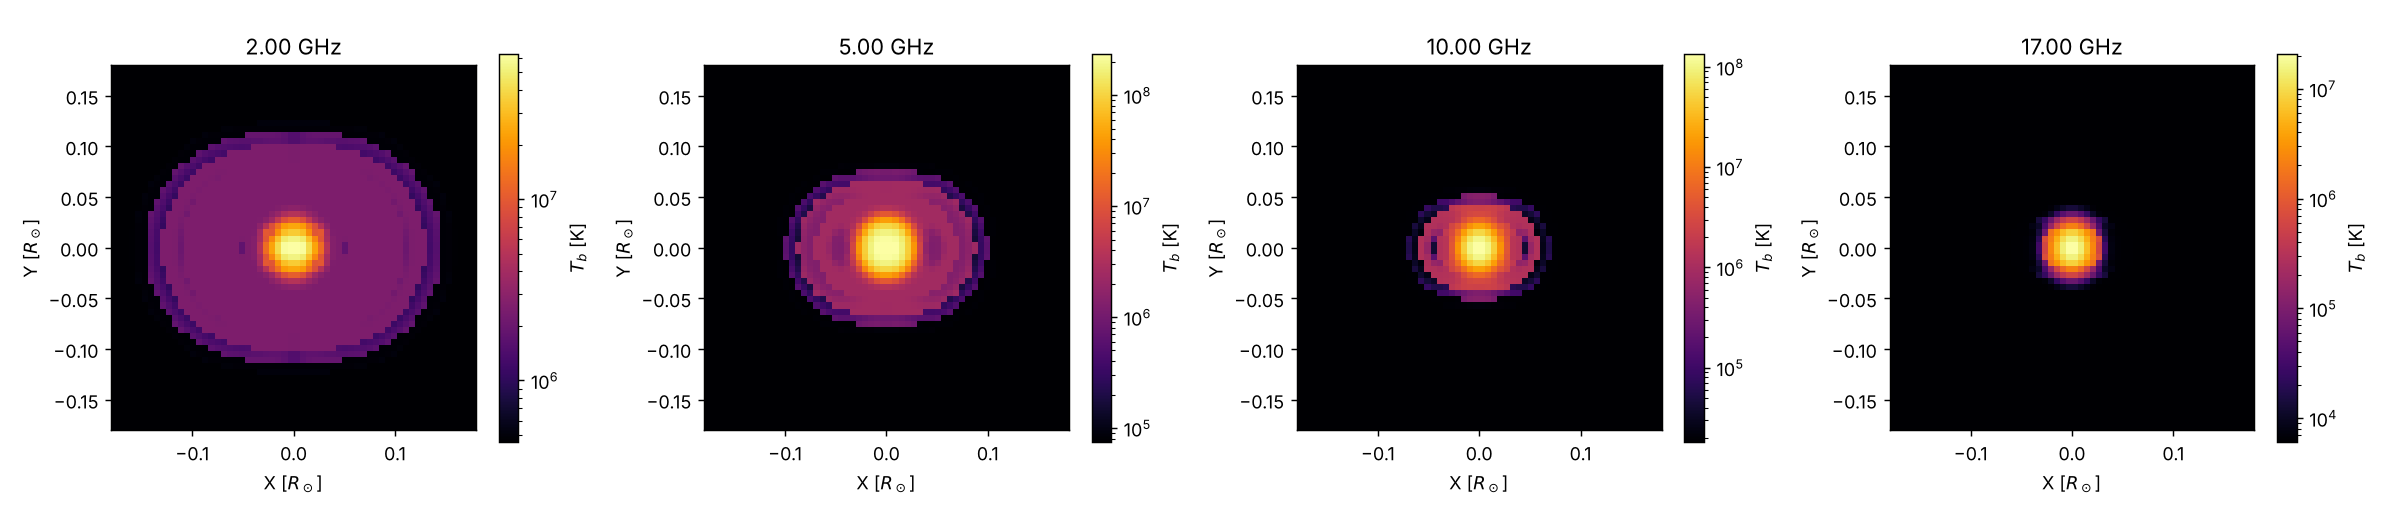
\includegraphics[width=\textwidth]{fig/cb_tb.png}\\[-1mm]
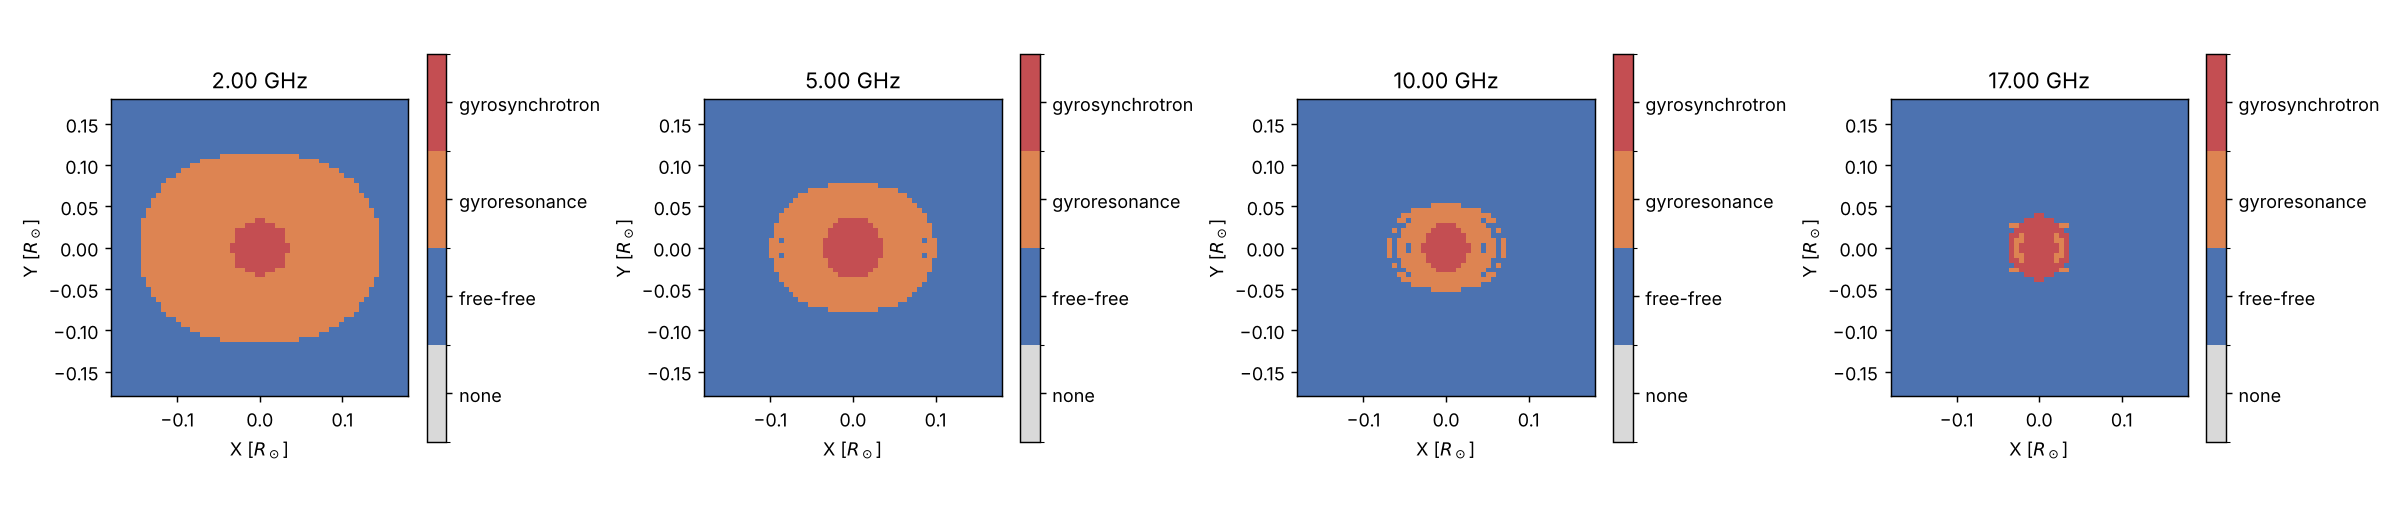
\includegraphics[width=\textwidth]{fig/cb_mechanism.png}
\caption{Combined image at 2, 5, 10 and 17\,GHz: $T_b$ (top) and the dominant process in
each pixel (bottom).}\label{fig:cbimg}
\end{figure}

\begin{figure}[h]\centering
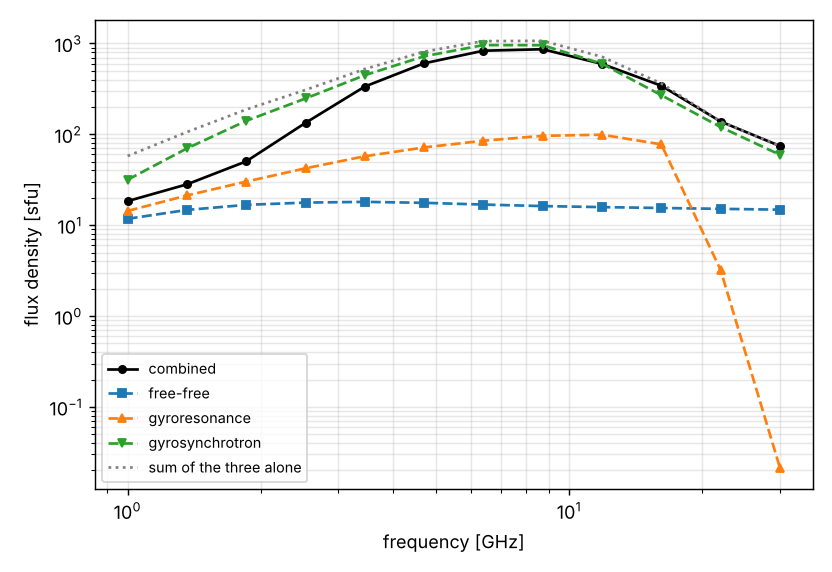
\includegraphics[width=0.62\textwidth]{fig/cb_spectrum.png}
\caption{Flux spectrum of the combined image compared with each process alone and with
the sum of the three.}\label{fig:cbspec}
\end{figure}

Figure~\ref{fig:cbimg} shows the gyrosynchrotron source in the centre, the thick
gyroresonance layers around it and free--free emission outside. The spectrum
(Figure~\ref{fig:cbspec}) shows why the transfer has to be done together: below
$\sim$4\,GHz the combined flux is far below the sum of the three, and even below the
gyrosynchrotron flux alone, because the $s=3$ and $s=4$ layers of the active region lie
\emph{above} the fast electrons and absorb their emission; at high frequencies the layers
retreat into the strong-field core and the processes simply add.

\section{Limitations}
\begin{itemize}[itemsep=1pt]
\item Straight rays (with the optional refraction correction of the free--free part).
\item Each voxel with fast electrons is treated by the codes as homogeneous; its
  gyrosynchrotron opacity is added to radiosynth's free--free and layers, and the codes'
  treatment of the refractive index inside the voxel is kept.
\item Mode coupling is treated by radiosynth (weak or strong), as for gyroresonance.
\item The fast electrons are prescribed (Chapter~\ref{chap:gs}).
\end{itemize}

%======================================================================
\chapter{Accuracy, performance and troubleshooting}
%======================================================================

\section{Accuracy}
\begin{itemize}[itemsep=2pt]
\item \textbf{Model resolution} matters most. Near the critical layer the ray bends on
      the density scale height, which is about 0.1\,\rsun{} in the low corona. Cells of
      0.02--0.05\,\rsun{} give results accurate to about 1\%
      (Chapter~\ref{chap:validation}).
\item \textbf{\code{step\_factor}}: the step follows the local cell size. Halving it
      checks convergence; in the tests the flux changed by $3\times10^{-4}$.
\item \textbf{Gyroresonance}: the layer optical depth depends on $L_B$, which is taken from
      $|B|$ at neighbouring sample points; the model must resolve the field scale
      ($\gtrsim$5 cells per $L_B$). Images converge to 1--2\% with the grid
      (Chapter~\ref{chap:validation}).
\item \textbf{Trilinear interpolation} of a steep profile slightly overestimates $n_e$
      between grid points. This is the same as in BATS-R-US.
\end{itemize}

\section{Performance}
The tracer advances all rays together with vectorised NumPy operations. On one core,
$128^2$ rays through a $200^3$ grid take about 2\,s per frequency. Time grows linearly
with the number of pixels and inversely with the cell size. \code{n\_workers} splits
the rays over processes, which share the grid in memory through \code{fork}. Memory is
about $20\,N_\text{cells}$ bytes in \code{float32}, e.g.\ 160\,MB for $200^3$.

\section{Troubleshooting}
\begin{description}[style=nextline,itemsep=3pt]
\item[The image is black or the flux is tiny] Check the printed $n_e$ and $T_e$. The
      units are probably wrong; set \code{--density-unit} or the PLUTO units. Also
      check that the observer is outside the domain and that the field of view covers
      the Sun.
\item[Brightness temperature higher than $T_e$] You are using \code{transfer="thin"},
      the BATS-R-US convention (Section~\ref{sec:transfer}).
\item[Many ``missed grid'' rays] The field of view is larger than the model domain.
      This is harmless, because those pixels see no plasma.
\item[``inner radius is \ldots{} R\_sun -- check UNIT\_LENGTH''] \code{definitions.h} was
      not found. Pass \code{definitions=} or \code{unit\_length=6.96e10}.
\item[Disk dark at GHz frequencies] The model has no chromosphere or transition region,
      so the corona is optically thin there. Lower the inner boundary or add a
      chromospheric model.
\item[Slow resampling] Use a BATS-R-US \code{box} plot, \code{resample\_method="nearest"},
      or a smaller \code{resample\_box}, and save the grid with \code{--save-grid}.
\item[Windows] Multiprocessing needs \code{fork}; on Windows use \code{n\_workers=1} or WSL.
\end{description}

\section{Limitations}
\begin{itemize}[itemsep=1pt]
\item Thermal free--free and gyroresonance emission are implemented, and gyrosynchrotron
      emission of prescribed fast electrons through the public fast GS codes. Plasma
      emission (type II/III bursts) and scattering by density turbulence
      (important below about 200\,MHz) are not included.
\item In the refractive tracer magneto-ionic effects are neglected: the refractive index
      is that of an unmagnetised plasma, as in BATS-R-US. Polarisation is computed only by
      the (straight-ray) gyroresonance package; its approximations are listed in
      Section~\ref{sec:grlimits}.
\item $T_b$ is the Rayleigh--Jeans brightness temperature. Flux densities assume a
      small field of view, $\Delta\Omega=\Delta X\Delta Y/D^2$.
\end{itemize}
